\documentclass[handout,babel,german,aspectratio=169]{beamer}
%%%%%%%%%%%%%%%%%%%%%%%%%%%%%%%%%%%%%%%%%%%%%%%%%%%%%%%%%%%%%%%%%%%
%                 Erstellt von Matthias Duch 2017                 %
%%%%%%%%%%%%%%%%%%%%%%%%%%%%%%%%%%%%%%%%%%%%%%%%%%%%%%%%%%%%%%%%%%%
\usepackage[ngerman]{babel}\usepackage[babel=true]{microtype}
\usepackage[utf8]{inputenc}%Without utf8x
\usepackage[T1]{fontenc}\usepackage{lmodern}\usepackage{url}\usepackage{color}\usepackage{tikz}\usetikzlibrary{shadows,arrows,shapes,calc}
\usepackage{amsmath,amssymb,amsfonts,amsthm,amsbsy}%$\varmathbb{R}$
\usepackage{graphicx} %\includegraphics[width=0.7\textwidth]{bild.jpg}
\usepackage{placeins} %for \FloatBarrier
\usepackage{setspace}
\usepackage{comment}
\usepackage{hyperref}
\usepackage{listings}
\usepackage{caption}
\usepackage{multicol}
\usepackage{xcolor}
%remove the icon
\setbeamertemplate{bibliography item}{}
%remove line breaks
\setbeamertemplate{bibliography entry title}{}
\setbeamertemplate{bibliography entry location}{}
\setbeamertemplate{bibliography entry note}{}

\newcommand*\keystroke[1]{\tikz[baseline=(key.base)]\node[draw, fill=white, drop shadow={shadow xshift=0.25ex,shadow yshift=-0.25ex,fill=black,opacity=0.75}, rectangle, rounded corners=2pt, inner sep=1pt, line width=0.5pt, font=\scriptsize\sffamily ](key) {#1\strut};}

\newsavebox{\codebox}% For saving code

%%%%%%%%%%%%%%%%%%%%%%%%%%%%%%%%%%%%%%%%%%%%%%%%%%%%%%%%%%%%%%%%%%%
%                            Themeneinstellungen                  %
%%%%%%%%%%%%%%%%%%%%%%%%%%%%%%%%%%%%%%%%%%%%%%%%%%%%%%%%%%%%%%%%%%%
\usetheme{Madrid}
\usecolortheme{beaver}
\setbeamertemplate{navigation symbols}{}%remove navigation symbols
\makeatletter
\setbeamertemplate{footline}
{
  \leavevmode%
  \hbox{%
  \begin{beamercolorbox}[wd=.333333\paperwidth,ht=2.25ex,dp=1ex,center]{author in head/foot}%
    \usebeamerfont{author in head/foot}\inserttitle
  \end{beamercolorbox}%
  \begin{beamercolorbox}[wd=.333333\paperwidth,ht=2.25ex,dp=1ex,center]{title in head/foot}%
    \usebeamerfont{title in head/foot}\insertsection
  \end{beamercolorbox}%
  \begin{beamercolorbox}[wd=.333333\paperwidth,ht=2.25ex,dp=1ex,right]{date in head/foot}%
    \usebeamerfont{date in head/foot}\insertshortdate{}\hspace*{2em}
    \insertframenumber{} / \inserttotalframenumber\hspace*{2ex} 
  \end{beamercolorbox}}%
  \vskip0pt%
}

\newcommand\blfootnote[1]{%
  \begingroup
  \renewcommand\thefootnote{}\footnote{#1}%
  \addtocounter{footnote}{-1}%
  \endgroup
}
\addto\captionsngerman{%Abkürzen der Überschriften
\renewcommand{\figurename}{Abb.}
\renewcommand{\tablename}{Tab.}
}
\usepackage{framed}
\newcommand\result[1]{\begin{framed}#1\end{framed}}



% make bullets red fit to theme
\definecolor{themenrot}{RGB}{163,0,0}
\definecolor{themengruen}{RGB}{0,82,41}
%%%%%%%%%%%%%%%%%%%%%%%%%%%%%%%%%%%%%%%%%%%%%%%%%%%%%%%%%%%%%%%%%%%
%                 Erstellt von Matthias Duch 2017                 %
%                                                                 %
% Programmiersprachen: (ausser den Standardsprachen)              %
% LaTeX, R, Stata                                                 %
%    \%%%%%%%%%%%%%%%%%%%%%%%%%%%%%%%%%%%%%%%%%%%%%%%%%%%%%%%%%%%%%%%%%%%
%                 Erstellt von Matthias Duch 2017                 %
%                                                                 %
% Programmiersprachen: (ausser den Standardsprachen)              %
% LaTeX, R, Stata                                                 %
%    \\input{../1.Vorlesung/Folien/settingsListing}               %
%%%%%%%%%%%%%%%%%%%%%%%%%%%%%%%%%%%%%%%%%%%%%%%%%%%%%%%%%%%%%%%%%%%
\usepackage{listings}
\definecolor{yellow}{RGB}{181,137,0}
\definecolor{red}{RGB}{220,50,47}
\definecolor{violet}{RGB}{108,113,196}
\definecolor{green}{rgb}{0,0.6,0}
\definecolor{gray}{rgb}{0.5,0.5,0.5}

\definecolor{Rblue}{HTML}{0000FF}
\definecolor{myblue}{HTML}{0000FF}




\newcommand{\colcomment}{\color{green}}
\newcommand{\colkeyword}{\color{blue}}
\newcommand{\coltexelem}{\color{green}}
\newcommand{\colnumbers}{\color{gray}}
\newcommand{\colstrings}{\color{violet}}
\newcommand{\colbackgrd}{\color{white}}

\lstset{literate= % Sonderzeichen ersetzen
  {á}{{\'a}}1 {é}{{\'e}}1 {í}{{\'i}}1 {ó}{{\'o}}1 {ú}{{\'u}}1
  {Á}{{\'A}}1 {É}{{\'E}}1 {Í}{{\'I}}1 {Ó}{{\'O}}1 {Ú}{{\'U}}1
  {à}{{\`a}}1 {è}{{\`e}}1 {ì}{{\`i}}1 {ò}{{\`o}}1 {ù}{{\`u}}1
  {À}{{\`A}}1 {È}{{\'E}}1 {Ì}{{\`I}}1 {Ò}{{\`O}}1 {Ù}{{\`U}}1
  {ä}{{\"a}}1 {ë}{{\"e}}1 {ï}{{\"i}}1 {ö}{{\"o}}1 {ü}{{\"u}}1
  {Ä}{{\"A}}1 {Ë}{{\"E}}1 {Ï}{{\"I}}1 {Ö}{{\"O}}1 {Ü}{{\"U}}1
  {â}{{\^a}}1 {ê}{{\^e}}1 {î}{{\^i}}1 {ô}{{\^o}}1 {û}{{\^u}}1
  {Â}{{\^A}}1 {Ê}{{\^E}}1 {Î}{{\^I}}1 {Ô}{{\^O}}1 {Û}{{\^U}}1
  {œ}{{\oe}}1 {Œ}{{\OE}}1 {æ}{{\ae}}1 {Æ}{{\AE}}1 {ß}{{\ss}}1
  {ű}{{\H{u}}}1 {Ű}{{\H{U}}}1 {ő}{{\H{o}}}1 {Ő}{{\H{O}}}1
  {ç}{{\c c}}1 {Ç}{{\c C}}1 {ø}{{\o}}1 {å}{{\r a}}1 {Å}{{\r A}}1
  {€}{{\euro}}1 {£}{{\pounds}}1 {«}{{\guillemotleft}}1
  {»}{{\guillemotright}}1 {ñ}{{\~n}}1 {Ñ}{{\~N}}1 {¿}{{?`}}1
}

\usepackage{accsupp}    
\lstset {
    numberstyle=\tiny\noncopynumber,
}

\newcommand{\noncopynumber}[1]{
    \BeginAccSupp{method=escape,ActualText={}}
    #1
    \EndAccSupp{}
}

% globale Einstellungen
\lstset{ %
  backgroundcolor=\colbackgrd,   % choose the background color; 
  basicstyle=\footnotesize,        % the size of the fonts that are used for the code
  breakatwhitespace=false,         % sets if automatic breaks should only happen at whitespace
  breaklines=true,                 % sets automatic line breaking
  emptylines=1, 
  captionpos=b,                    % sets the caption-position to bottom
  commentstyle=\itshape\colcomment,    % comment style
  deletekeywords={...},            % if you want to delete keywords from the given language
 % escapeinside={\%*}{*)},          % if you want to add LaTeX within your code
  extendedchars=true,              % lets you use non-ASCII characters; for 8-bits encodings only, does not work with UTF-8
  frame=single,	                   % adds a frame around the code
  keepspaces=true,                 % keeps spaces in text, useful for keeping indentation of code (possibly needs columns=flexible)
  keywordstyle=\colkeyword,       % keyword style
  otherkeywords={*,...},           % if you want to add more keywords to the set
  numbers=left,                    % where to put the line-numbers; possible values are (none, left, right)
  numbersep=1pt,                   % how far the line-numbers are from the code
  numberstyle=\sffamily\tiny\color{red!90}\noncopynumber, % the style that is used for the line-numbers
  numberfirstline=true,
  rulecolor=\color{black!70},         % if not set, the frame-color may be changed on line-breaks within not-black text (e.g. comments (green here))
  showspaces=false,                % show spaces everywhere adding particular underscores; it overrides 'showstringspaces'
  showstringspaces=false,          % underline spaces within strings only
  showtabs=false,                  % show tabs within strings adding particular underscores  showtabs=false,                 , % show tabs within strings adding particular underscores
  stepnumber=1,                    % the step between two line-numbers. If it's 1, each line will be numbered
  stringstyle=\colstrings,     % string literal style
  tabsize=2,	                   % sets default tabsize to 2 spaces
  title=\lstname,                   % show the filename of files included with \lstinputlisting; also try caption instead of title
  xleftmargin=3.4pt, % Einschub, durch die Zeilennummerierung bedingt
  xrightmargin=3.4pt,
  %
  alsoletter={.},
  %
  basicstyle=\ttfamily\color{black}, 
  columns=flexible,
}

%%%%%%%%%%%%%%%%%%%%%%%%%%%%%%%%%%%%%%%%%%%%%%%%%%%%%%%%%%%%%%%%%%%
%                           Sprachdefinitionen                    %
%%%%%%%%%%%%%%%%%%%%%%%%%%%%%%%%%%%%%%%%%%%%%%%%%%%%%%%%%%%%%%%%%%%

\lstdefinelanguage{Stata}{
    morekeywords=,
    morekeywords=[2]{cntrade, chinafin, wbopendata, spmap,},
    morekeywords=[3]{regress, summarize, display,},
    morekeywords=[4]{forvalues, if, foreach, set},
    morekeywords=[5]{rnormal, runiform},
    morecomment=[l]{//},
    morecomment=[s]{/*}{*/},
    % The following is used by macros, like `lags'.
    morecomment=[n][keywordstyle]{`}{'},
    morestring=[b]",
    sensitive=true,
}

\lstdefinestyle{Stata}{
  language=Stata,
  keywordstyle=\color{black},
  moredelim=**[is][\color{red}]{@}{@},
}

\lstdefinestyle{R}{%eigentlich nur R, aber aus Kompatibilitat zu alten Versionen
  style=base
}
\newcommand{\CodeSymbol}[1]{\textcolor{red}{#1}}

\lstdefinestyle{base}{
  language=R,
  emptylines=1,
  breaklines=true,
  alsoletter={.},
  basicstyle=\ttfamily\color{black},
  keywordstyle=\color{black},
  moredelim=**[is][\color{red}]{@}{@},
  %otherkeywords={<-,!,!=,~,$,*,\&,+,^,\%,\%/\%,\%*\%,\%\%,<<-,_,/},
%  morekeywords=,
%  morekeywords=[2]{+, chinafin, wbopendata, spmap,},
}

\lstdefinestyle{Latex}{
  language={[LaTeX]TeX},
  %
  moretexcs={geometry, definecolor, textcolor, colorbox, color, pagecolor, fcolorbox, setlength, tableofcontents, subsection, subsubsection, thepage, includegraphics, listoftables, citet, citep, eqref, fnysmbol, nameref, listoffigures, listoftables, url, href, printindex, blindtext, pause, titlepage, frametitle, subtitle, titlepage, usetheme,}, % define Commands
  morekeywords={maketitle}, %Keywords
  %
  texcsstyle=*\coltexelem, % Commandstyle
  moredelim=**[s][\color{yellow}]{[}{]},
}

%Patch issue, that closing parenthesis is not colored, if breaklines=True


               %
%%%%%%%%%%%%%%%%%%%%%%%%%%%%%%%%%%%%%%%%%%%%%%%%%%%%%%%%%%%%%%%%%%%
\usepackage{listings}
\definecolor{yellow}{RGB}{181,137,0}
\definecolor{red}{RGB}{220,50,47}
\definecolor{violet}{RGB}{108,113,196}
\definecolor{green}{rgb}{0,0.6,0}
\definecolor{gray}{rgb}{0.5,0.5,0.5}

\definecolor{Rblue}{HTML}{0000FF}
\definecolor{myblue}{HTML}{0000FF}




\newcommand{\colcomment}{\color{green}}
\newcommand{\colkeyword}{\color{blue}}
\newcommand{\coltexelem}{\color{green}}
\newcommand{\colnumbers}{\color{gray}}
\newcommand{\colstrings}{\color{violet}}
\newcommand{\colbackgrd}{\color{white}}

\lstset{literate= % Sonderzeichen ersetzen
  {á}{{\'a}}1 {é}{{\'e}}1 {í}{{\'i}}1 {ó}{{\'o}}1 {ú}{{\'u}}1
  {Á}{{\'A}}1 {É}{{\'E}}1 {Í}{{\'I}}1 {Ó}{{\'O}}1 {Ú}{{\'U}}1
  {à}{{\`a}}1 {è}{{\`e}}1 {ì}{{\`i}}1 {ò}{{\`o}}1 {ù}{{\`u}}1
  {À}{{\`A}}1 {È}{{\'E}}1 {Ì}{{\`I}}1 {Ò}{{\`O}}1 {Ù}{{\`U}}1
  {ä}{{\"a}}1 {ë}{{\"e}}1 {ï}{{\"i}}1 {ö}{{\"o}}1 {ü}{{\"u}}1
  {Ä}{{\"A}}1 {Ë}{{\"E}}1 {Ï}{{\"I}}1 {Ö}{{\"O}}1 {Ü}{{\"U}}1
  {â}{{\^a}}1 {ê}{{\^e}}1 {î}{{\^i}}1 {ô}{{\^o}}1 {û}{{\^u}}1
  {Â}{{\^A}}1 {Ê}{{\^E}}1 {Î}{{\^I}}1 {Ô}{{\^O}}1 {Û}{{\^U}}1
  {œ}{{\oe}}1 {Œ}{{\OE}}1 {æ}{{\ae}}1 {Æ}{{\AE}}1 {ß}{{\ss}}1
  {ű}{{\H{u}}}1 {Ű}{{\H{U}}}1 {ő}{{\H{o}}}1 {Ő}{{\H{O}}}1
  {ç}{{\c c}}1 {Ç}{{\c C}}1 {ø}{{\o}}1 {å}{{\r a}}1 {Å}{{\r A}}1
  {€}{{\euro}}1 {£}{{\pounds}}1 {«}{{\guillemotleft}}1
  {»}{{\guillemotright}}1 {ñ}{{\~n}}1 {Ñ}{{\~N}}1 {¿}{{?`}}1
}

\usepackage{accsupp}    
\lstset {
    numberstyle=\tiny\noncopynumber,
}

\newcommand{\noncopynumber}[1]{
    \BeginAccSupp{method=escape,ActualText={}}
    #1
    \EndAccSupp{}
}

% globale Einstellungen
\lstset{ %
  backgroundcolor=\colbackgrd,   % choose the background color; 
  basicstyle=\footnotesize,        % the size of the fonts that are used for the code
  breakatwhitespace=false,         % sets if automatic breaks should only happen at whitespace
  breaklines=true,                 % sets automatic line breaking
  emptylines=1, 
  captionpos=b,                    % sets the caption-position to bottom
  commentstyle=\itshape\colcomment,    % comment style
  deletekeywords={...},            % if you want to delete keywords from the given language
 % escapeinside={\%*}{*)},          % if you want to add LaTeX within your code
  extendedchars=true,              % lets you use non-ASCII characters; for 8-bits encodings only, does not work with UTF-8
  frame=single,	                   % adds a frame around the code
  keepspaces=true,                 % keeps spaces in text, useful for keeping indentation of code (possibly needs columns=flexible)
  keywordstyle=\colkeyword,       % keyword style
  otherkeywords={*,...},           % if you want to add more keywords to the set
  numbers=left,                    % where to put the line-numbers; possible values are (none, left, right)
  numbersep=1pt,                   % how far the line-numbers are from the code
  numberstyle=\sffamily\tiny\color{red!90}\noncopynumber, % the style that is used for the line-numbers
  numberfirstline=true,
  rulecolor=\color{black!70},         % if not set, the frame-color may be changed on line-breaks within not-black text (e.g. comments (green here))
  showspaces=false,                % show spaces everywhere adding particular underscores; it overrides 'showstringspaces'
  showstringspaces=false,          % underline spaces within strings only
  showtabs=false,                  % show tabs within strings adding particular underscores  showtabs=false,                 , % show tabs within strings adding particular underscores
  stepnumber=1,                    % the step between two line-numbers. If it's 1, each line will be numbered
  stringstyle=\colstrings,     % string literal style
  tabsize=2,	                   % sets default tabsize to 2 spaces
  title=\lstname,                   % show the filename of files included with \lstinputlisting; also try caption instead of title
  xleftmargin=3.4pt, % Einschub, durch die Zeilennummerierung bedingt
  xrightmargin=3.4pt,
  %
  alsoletter={.},
  %
  basicstyle=\ttfamily\color{black}, 
  columns=flexible,
}

%%%%%%%%%%%%%%%%%%%%%%%%%%%%%%%%%%%%%%%%%%%%%%%%%%%%%%%%%%%%%%%%%%%
%                           Sprachdefinitionen                    %
%%%%%%%%%%%%%%%%%%%%%%%%%%%%%%%%%%%%%%%%%%%%%%%%%%%%%%%%%%%%%%%%%%%

\lstdefinelanguage{Stata}{
    morekeywords=,
    morekeywords=[2]{cntrade, chinafin, wbopendata, spmap,},
    morekeywords=[3]{regress, summarize, display,},
    morekeywords=[4]{forvalues, if, foreach, set},
    morekeywords=[5]{rnormal, runiform},
    morecomment=[l]{//},
    morecomment=[s]{/*}{*/},
    % The following is used by macros, like `lags'.
    morecomment=[n][keywordstyle]{`}{'},
    morestring=[b]",
    sensitive=true,
}

\lstdefinestyle{Stata}{
  language=Stata,
  keywordstyle=\color{black},
  moredelim=**[is][\color{red}]{@}{@},
}

\lstdefinestyle{R}{%eigentlich nur R, aber aus Kompatibilitat zu alten Versionen
  style=base
}
\newcommand{\CodeSymbol}[1]{\textcolor{red}{#1}}

\lstdefinestyle{base}{
  language=R,
  emptylines=1,
  breaklines=true,
  alsoletter={.},
  basicstyle=\ttfamily\color{black},
  keywordstyle=\color{black},
  moredelim=**[is][\color{red}]{@}{@},
  %otherkeywords={<-,!,!=,~,$,*,\&,+,^,\%,\%/\%,\%*\%,\%\%,<<-,_,/},
%  morekeywords=,
%  morekeywords=[2]{+, chinafin, wbopendata, spmap,},
}

\lstdefinestyle{Latex}{
  language={[LaTeX]TeX},
  %
  moretexcs={geometry, definecolor, textcolor, colorbox, color, pagecolor, fcolorbox, setlength, tableofcontents, subsection, subsubsection, thepage, includegraphics, listoftables, citet, citep, eqref, fnysmbol, nameref, listoffigures, listoftables, url, href, printindex, blindtext, pause, titlepage, frametitle, subtitle, titlepage, usetheme,}, % define Commands
  morekeywords={maketitle}, %Keywords
  %
  texcsstyle=*\coltexelem, % Commandstyle
  moredelim=**[s][\color{yellow}]{[}{]},
}

%Patch issue, that closing parenthesis is not colored, if breaklines=True



\captionsetup{justification=centering}
%\setbeamercolor*{item}{fg=themenrot}%make bullets red fit to redtheme
\setbeamercolor*{item}{fg=themengruen}%make bullets red fit to greentheme
\newcommand{\code}[1]{\texttt{#1}}
\newcommand{\bcode}[1]{\texttt{\textbf{#1}}} %fetter Code
\newcommand{\ccode}[1]{\begin{center}\texttt{\textbf{\Large{#1}}}\end{center}} 
\makeatother

% gruenes Thema
\usecolortheme{spruce}% gruenes Theme



%%%%%%%%%%%%%%%%%%%%%%%%%%%%%%%%%%%%%%%%%%%%%%%%%%%%%%%%%%%%%%%%%%%%%%%%%%%%%%%%%%%%%%%%%%%%%%%%%%%%%%%%%%%
%                      Einstellungen fuer die Uebersicht am Anfang jedes Kapitels                         %
%%%%%%%%%%%%%%%%%%%%%%%%%%%%%%%%%%%%%%%%%%%%%%%%%%%%%%%%%%%%%%%%%%%%%%%%%%%%%%%%%%%%%%%%%%%%%%%%%%%%%%%%%%%
\AtBeginSection[]{
\begin{frame}<beamer|handout>
\frametitle{Übersicht}
\tableofcontents[currentsection,hideallsubsections]
\end{frame}}
%Übersicht am Anfang einer Subsection
\AtBeginSubsection[]{
\begin{frame}<beamer|handout>
\frametitle{Übersicht}
\tableofcontents[currentsection,hideothersubsections,sectionstyle=show/hide,        subsectionstyle=show/shaded/hide]
\end{frame}}



%%%%%%%%%%%%%%%%%%%%%%%%%%%%%%%%%%%%%%%%%%%%%%%%%%%%%%%%%%%%%%%%%%%%%%%%%%%
%                         Design fuer Aufzahlungen                        %
%%%%%%%%%%%%%%%%%%%%%%%%%%%%%%%%%%%%%%%%%%%%%%%%%%%%%%%%%%%%%%%%%%%%%%%%%%%
%         Design fuer Aufzahlungen       %
\setbeamertemplate{sections/subsections in toc}[square]
\setbeamertemplate{enumerate items}[square]
\setbeamertemplate{itemize items}[square]



%%%%%%%%%%%%%%%%%%%%%%%%%%%%%%%%%%%%%%%%%%%%%%%%%%%%%%%%%%%%%%%%%%%%%%%%%%%
%                         Angaben auf den Folien                          %
%%%%%%%%%%%%%%%%%%%%%%%%%%%%%%%%%%%%%%%%%%%%%%%%%%%%%%%%%%%%%%%%%%%%%%%%%%%
\title{Einführung in \LaTeX~2017} 
\author{Matthias Duch und Dennis Kubitza}
\date{Juli 2017}
\newtheorem{satz}{Satz}[section]
 %Für Math und Referenzen
%\newcommand{\ins}[1]{\chead{#1} \input{#1} \newpage}%ohne das gibt es nen Fehler.....



\begin{document}

\begin{frame}<handout:0>% Die erste Folie muss bleiben. Sonst funktioniert nichts...
	\visible<1>{\titlepage}
	\frametitle{Matthias und Dennis präsentieren:}
	\pause% es hängt an diesem Pause Befehl.... ohne den geht es sonst nicht
	\vspace{-70mm}
	% jetzt kommt noch eine Logoseite. Dann klappt alles wie gewohnt.
	\visible<2->{\center{
\includegraphics[width=0.6\textwidth]{images/LaTeX_logo.png}}}
\end{frame}


\section{Grundlagen}
\subsection{Organisatorisches}

\begin{frame}
\frametitle{Ziele dieses Kurses}
\begin{itemize}[<+->]
  \item Grundsätzliches Verständnis von \LaTeX
  \item Verfassen von wissenschaftlichen Schriften (z.B. Bachelor/Masterarbeit)
  \item Erstellen von Präsentationen
\end{itemize}
\end{frame}

\begin{frame}
\frametitle{Kursinformationen}
\begin{itemize}
\item Dozenten:
\begin{enumerate}
\item Matthias Duch (s6maduch@uni-bonn.de)
\item Dennis Kubitza (s6dekubi@uni-bonn.de)
\end{enumerate} 
\pause
\item Kursunterlagen: \\
Die Kursunterlagen werden parallel zum Kurs hochgeladen und geupdated. Ihr findet dort die Folien, die Übungszettel und später auch Musterlösungen: \\ \ \\
\centering\scalebox{1}{\url{https://www.fs-vwl.uni-bonn.de/de/latexkurs/latexkurs}}
\end{itemize}
\end{frame}

\begin{frame}
\frametitle{Organisatorisches}
Der Kurs gliedert sich in zwei Teile:
\begin{itemize}[<+->]
  \item  Vorlesung: %11-13 Uhr (Gr. HS)
   \begin{itemize}[<+->]
   \item Fr: 17-20 Uhr (hier)
   \item Sa: 10-18 Uhr (hier)
   \item So: 10-18 Uhr (hier)
   \end{itemize}
  \item  Die Übungen finden nach dem Durchsprechen der Folien statt.
  \item  Besprechung der Übungen: Am Anfang des nächsten Tages/ Sonntag Abends.
\end{itemize}
\end{frame}

\subsection{Infos über \LaTeX}


\begin{frame}
\frametitle{Was ist \LaTeX?}
\begin{itemize}[<+->]
  \item \TeX\, ist ein von Donald E. Knuth entwickeltes Textsatzsystem. Es ist schwierig zu benutzen, erlaubt jedoch die Erstellung von Makropaketen. Diese erlauben es eine einfachere Syntax zu verwenden
  \item \LaTeX\, ist ein von Leslie Lamport entwickeltes Makropaket, das in \TeX~ geschrieben wurde. Es stellt eine einfache Kommandostruktur zur Verfügung, dabei können mit vertieften \LaTeX~ Kenntnissen alle Einstellungen individuell verändert werden.
  \item PDF\LaTeX~ Variante von \LaTeX~, die direkt eine PDF erstellt.
\end{itemize}
\end{frame}

\begin{frame}
\frametitle{Geschichtliches}
\begin{itemize}[<+->]
  \item[1982] \textbf{Donald E. Knuth}, Professor an der Stanford-University, veröffentlicht die erste Version von \TeX
  \item[1985] \textbf{Leslie Lamport} veröffentlicht eine darauf aufbauende erste Version des Systems \LaTeX, eine sehr mächtige Sammlung von \TeX-Makros.
    Der Name basiert auf \textbf{La}mport \textbf{\TeX}.
  \item[1993] \LaTeX $2_\epsilon$ wird als offizielle Version fertig gestellt.
  \item \LaTeX 3 befindet sich momentan in der Entwicklung.
\end{itemize}

\end{frame}

\begin{frame}
\frametitle{Warum \LaTeX}
\begin{itemize}[<+->]
  \item Hardware- und Betriebssystemunabhängig
  \item Trennung von Design und Inhalt
  \item Trennung von Editor und Compiler
  \item Textbild
  \item Formatierung von Formeln
  \item Skriptfähigkeit
  %\item ``echtes'' PDF 
\end{itemize}
\end{frame}

\begin{frame}
\frametitle{Quellen}
\begin{itemize}[<+->]
  \item www.ctan.org: The Comprehensive \TeX-Archive Network
  \item Helmut Kopka: \LaTeX, Band 1: Einführung
  \item Suche im Internet
\end{itemize}
\end{frame}

\begin{frame}
\frametitle{Was benötige ich?}
\begin{itemize}[<+->]
\item Compiler (z.B. TeXLive)
\item Editor (z.B. TeXMaker, ...)
\item Viewer (z.B. Adobe Acrobat, ...)
\end{itemize}
\end{frame}


\subsection{Installation}

\begin{frame}
\frametitle{Installation}
Ihr findet eine Installationsanleitung auf unserer Homepage! Wir gehen diese nun durch während ihr alles installiert. Dann geht es weiter mit den Folien.

\end{frame}

\subsection{Erste Schritte}


\begin{frame}
\frametitle{Funktionsweise von \LaTeX}
\begin{center}
\begin{tikzpicture}[box/.style={rounded rectangle,draw},shorten >= 2pt]
    \node[box] at (0,0) (tf) {.tex}; \pause
    \node[box] at (3,0) (dvi) {.dvi};
    \draw[->] (tf.east) -- node[above,label=90:\texttt{latex}] {} (dvi.west); \pause
    \node[box] at (6,0) (ps) {.ps};
    \draw[->] (dvi.east) -- node[above,label=90:\texttt{dvips}] {} (ps.west); \pause
    \node[box] at (9,0) (pdf) {.pdf};
    \draw[->] (ps.east) -- node[above,label=90:\texttt{ps2pdf}] {} (pdf.west); \pause
    \draw[->,bend left] (tf.north) to node[above,label=90:\texttt{pdflatex}] {} (pdf.north);
\end{tikzpicture}
\end{center}
\end{frame}

\begin{frame}[fragile]
\frametitle{Aufbau einer \LaTeX-Dokumentes}
Jede \LaTeX-Datei besteht aus
\begin{itemize}[<+->]
  \item Der \emph{Vorspann} (preamble) ist für globale Einstellungen zuständig:
  \begin{itemize}
    \item Setzen von Variablen
    \item Laden von Bibliotheken
  \end{itemize}
  \item Er beginnt mit \lstinline[style=Latex]+\documentclass[...]{...}+ und endet mit \lstinline[style=Latex]+\begin{document}+
  \item Der \emph{Textteil} (body) beinhaltet den eigentlichen Text.
  \item Er beginnt mit \lstinline[style=Latex]+\begin{document}+ und endet mit \lstinline[style=Latex]+\end{document}+
\end{itemize}
\end{frame}

\begin{frame}[fragile]
\frametitle{Aufbau eines \LaTeX-Dokumentes}
Der Code
\begin{lstlisting}[style=Latex]
\documentclass{article}
\begin{document}
 Mein erstes Dokument in \LaTeX
\end{document}
\end{lstlisting} 
\pause
liefert uns das Ergebnis
\result{
Mein erstes Dokument in \LaTeX
}
\end{frame}

\begin{frame}[fragile]
\frametitle{Wichtige Befehlte für die Preambel}
Wir werden ab sofort mit einer Präambel arbeiten die weitere wichtige Einstellungen definiert: 
\begin{lstlisting}[style=Latex]
\documentclass[11pt,a4paper]{article}
\usepackage[ngerman]{babel}
\usepackage[utf8]{inputenc}
\usepackage[T1]{fontenc}
\usepackage{lmodern}
\usepackage[top=2cm, left=3cm, right=2cm, bottom=2cm]{geometry}
\begin{document}
 Mein erstes Dokument in \LaTeX
\end{document}
\end{lstlisting} 
\end{frame}


\begin{frame}[fragile]
\frametitle{Kommentare}
\begin{itemize}[<+->]
  \item Kommentare dienen der Übersicht
  \item mit Ihnen lassen sich Teile ausblenden, um Fehler zu finden
  \item ein Kommentar beginnt immer mit \lstinline[style=Latex]+%+
  \item die meisten Editoren bieten auch Shortcuts an, um mehrere Zeilen automatisch zu kommentieren
\end{itemize}\pause
\begin{lstlisting}[style=Latex]
% Dokument von Max Mustermann
Dieser Text ist sichtbar % sichtbarer Text
\end{lstlisting}
% Dokument von Max Mustermann
\vspace{-20pt}
\pause
\result{
Dieser Text ist sichtbar % sichtbarer Text
}
\end{frame}

\begin{frame}[fragile,t]
\frametitle{Zusammenfassung}
\begin{lstlisting}[style=Latex]
% erst der Vorspann
\documentclass[a4paper]{article}

[...]

% dann der Textteil.
\begin{document}
Heute ist der \today.
\end{document}
\end{lstlisting}
\pause
\vspace{-20pt}
\result{
Heute ist der \today.
}
\end{frame}
\begin{frame}[fragile]
\frametitle{Syntax}
\linespread{1.5}
In \LaTeX\, gibt es zwei wichtige Strukturen: \pause
\begin{itemize}[<+->]
  \item Befehle
  \item Umgebungen
\end{itemize}	
\end{frame}

\begin{frame}[fragile]
\frametitle{Befehle}
\linespread{1.5}
Jeder Befehl beginnt entweder mit einem Backslash ``\verb+\+'' (z.B. ``\lstinline[style=Latex]+\documentclass+'') 
oder ist ein Einzeichenbefehl: ``\texttt{\$,\%,\&,\#,\_}'' und einige mehr.\\ \pause
Dabei gilt als Faustregel:
\begin{itemize}[<+->]
  \item Obligatorische Argumente stehen in geschweiften Klammern (\lstinline[style=Latex]+{ }+)
  \item Optionale Argumente in eckigen Klammern (\lstinline[style=Latex]+[ ]+)
\end{itemize} \pause
\vfill
\begin{exampleblock}{Beispiele} \lstinline[style=Latex]+\documentclass[a4paper]{article}+ \\ \lstinline[style=Latex]+\today+
\end{exampleblock}
\end{frame}

\begin{frame}[fragile]
\frametitle{Wichtige Befehle für den Anfang}
\linespread{1.5}
\begin{itemize}
\item Zeilenumbrüche: \lstinline[style=Latex]+\\+ \\
\item Zeilenumbrüche von beliebiger Größe  \lstinline[style=Latex]+\\[1.2cm]+
\item nicht automatische Leerzeichen  \lstinline[style=Latex]+~+
\end{itemize}
Latex rückt Text nach einem Zeilenumbruch automatisch ein, wenn die darauf folgende Zeile leer ist. Dies kann man mit \lstinline[style=Latex]+\noindent+ verhindern.
Schreibt man mehrere Leerzeichen in die TeX. Datei, wertet der Compilier nur eines aus
\end{frame}

\begin{frame}[fragile]
\frametitle{Beispielcode}
 \begin{lstlisting}[style=Latex]
\begin{document}
In diesem Text wurden 5            Leerzeichen eingefügt. Ohne Effekt. 
Verwendet man Tilde ~~~~ sieht das Ganze schon anders aus. Testen wir nun einen Zeilenumbruch \\ 

Die leere Zeile führt dazu, dass Latex einrückt.\\

\noindent Dies können wir allerdings verhindern. Als letztes Versuchen wir noch einen großen Zeilenumbruch.\\[4cm]
Auch dieser klappt.


\end{document}
\end{lstlisting} 
\end{frame}
\begin{frame}[fragile,t]\vspace{-15pt}
\frametitle{Ergebnisse zu Umbrüchen, Leerzeichen}
\result{
~~~~~In diesem Text wurden 5            Leerzeichen eingefügt. Ohne Effekt. 
Verwendet man Tilde ~~~~ sieht das Ganze schon anders aus. Testen wir nun einen Zeilenumbruch \\ 

~~~~ Die leere Zeile führt dazu, dass Latex einrückt.\\

\noindent Dies können wir allerdings verhindern. Als letztes Versuchen wir noch einen großen Zeilenumbruch.\\[4cm]
Auch dieser klappt.}
\end{frame}
%-------------------------------------------------------------------------------
\begin{frame}[fragile]
\frametitle{Wichtige Befehle für den Anfang 2}
\linespread{1.5}
\begin{itemize}
\item fetter Text: \lstinline[style=Latex]+\textbf{<text>}+ \\
\item kursiver Text:  \lstinline[style=Latex]+\textit{<text>}+
\item Ausrichtungen:  \lstinline[style=Latex]+\flushright{<text>}\flushleft{<text>}\center{<text>}+
\end{itemize}
\end{frame}

\begin{frame}[fragile]
\frametitle{Beispielcode}
 \begin{lstlisting}[style=Latex]
\begin{document}
Wir heben nun einen Teil \textbf{des Textes durch einen Fettdruck vor.} Dies klappt natürlich auch für \textit{kursive Textabschnitte wie} diesen hier. Wollen wir nun unseren Text an verschiedenen Stellen positionieren, \flushright{können wir entweder rechtsbündig} \center{mittig} \flushleft{oder ganz normal linksbündig schreiben.} 
\end{document}
\end{lstlisting} 
\end{frame}
\begin{frame}[fragile]
\frametitle{Ergebnisse zu Text}
\result{
Wir heben nun einen Teil \textbf{des Textes durch einen Fettdruck vor.} Dies klappt natürlich auch für \textit{kursive Textabschnitte wie} diesen hier. Wollen wir nun unseren Text an verschiedenen Stellen positionieren, \flushright{können wir entweder rechtsbündig} \center{mittig} \flushleft{oder ganz normal linksbündig schreiben.} 
}
\end{frame}

\begin{frame}[fragile]
\frametitle{Strukturbefehle}
\linespread{1.5}
Die Wohl wichtigsten Befehle sind die Strukturbefehle in Latex. Sie Gliedern ein Dokument in Kapitel, Abschnitte, Unterabschnitte, Unterunterabschnitte etc, welche automatisch in ein Inhaltsverzeichnis überführt werden.
\begin{itemize}[<+->]
  \item Kapitel: \lstinline[style=Latex]+\section{<Titel>}+ \\
  \item Abschnitte:  \lstinline[style=Latex]+\subsection{<Untertitel>}+ 
  \item Unterabschnitte:  \lstinline[style=Latex]+\subsubsection{<Unteruntertitel>}+
\end{itemize}
Das Inhaltsverzeichnis kann mit \lstinline[style=Latex]+\tableofcontents+ angezeigt werden.
\end{frame}

\begin{frame}[fragile]
\frametitle{Beispielcode}
\begin{lstlisting}[style=Latex]
...
\begin{document}
\tableofcontents
\section{Ein neuer Abschnitt}
Hier könnt ihr ganz normal weiter schreiben. Hier könnt ihr ganz normal weiter schreiben. 
\subsection{Mit diesem Unterabschnitt}
Hier könnt ihr ganz normal weiter schreiben. Hier könnt ihr ganz normal weiter schreiben.
\subsection{Und einem Zweiten Unterabschnitt}
Hier könnt ihr ganz normal weiter schreiben.
\section{Neuer Abschnitt}
Man kann auch mehrere Abschnitte definieren. Beachtet bitte die Automatische Nummerierung. 
\end{document}
\end{lstlisting} 
\end{frame}

\begin{frame}[fragile]
\frametitle{Beispielcode}
\vspace{-70pt}
\begin{figure}[htp]
\centering
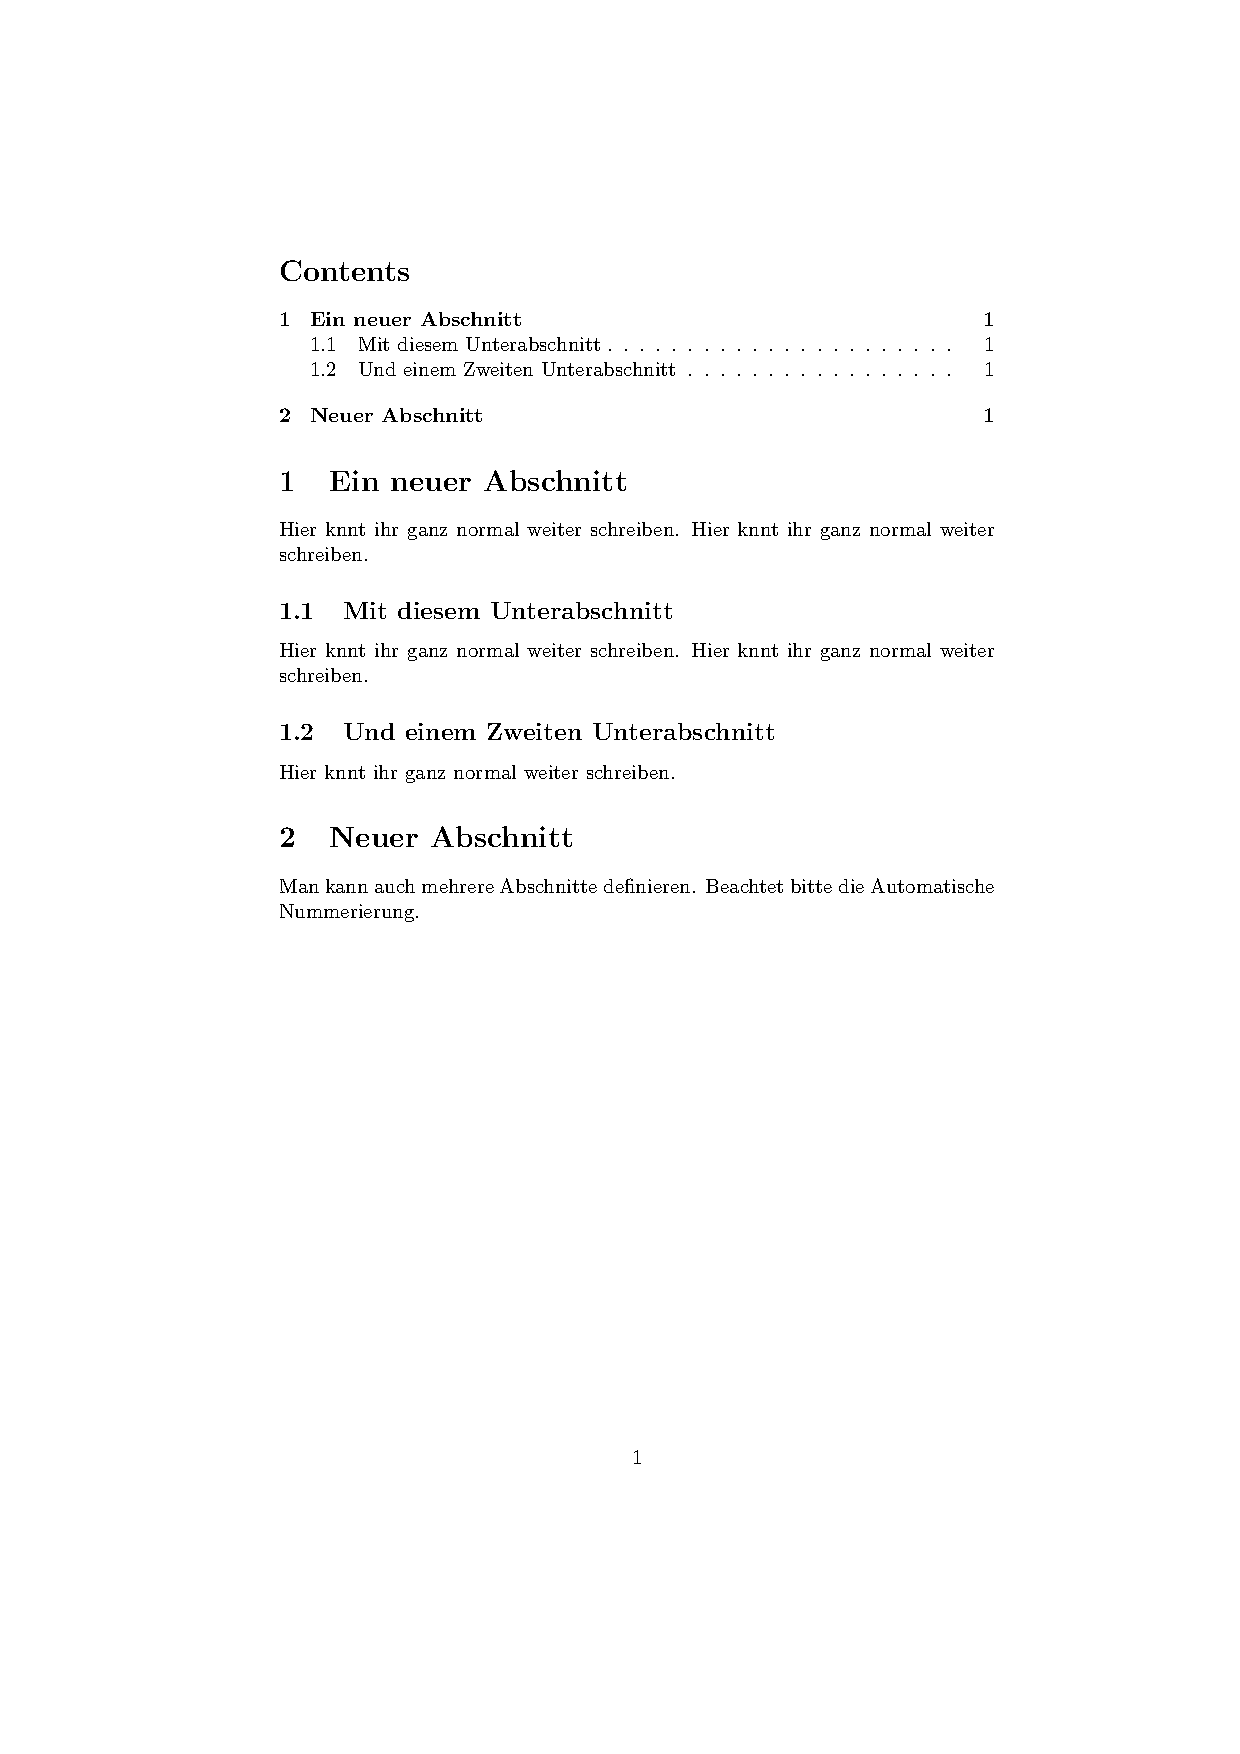
\includegraphics[scale=.6]{Beispiele/Sections/Bsp_section.pdf}
\caption{}
\label{}
\end{figure}
\end{frame}


\begin{frame}[fragile]
\frametitle{Syntax}
\linespread{1.5}
In \LaTeX\, gibt es zwei wichtige Strukturen: \pause
\begin{itemize}[<+->]
  \item Befehle
  \item Umgebungen
\end{itemize}	

\end{frame}

\begin{frame}[fragile]
\frametitle{Umgebungen}
\linespread{1.5}
Umgebungen werden benötigt, um dem Compiler zu sagen, was zusammen gehört. \pause
\begin{itemize}[<+->]
  \item Die einfachste Umgebung ist \lstinline[style=Latex]+{ }+ Diese haben wir in einigen Befehlen bereits benutzt.
  \item Es gibt auch sogenannte definierte Umgebungen. Diese werden durch
  	\begin{center}
\begin{lstlisting}[style=Latex] 
\begin{<Umgebung>}
\end{<Umgebung>}
\end{lstlisting}\end{center}\vspace{-30pt}
gekennzeichnet. Beispiele zu diesen definierten Umgebungen folgen morgen.
\end{itemize}
\end{frame}





% Tag 2
%\section{Textsatz}
\subsection{Klassen und Bibliotheken}

\begin{frame}[fragile,t]
\frametitle{Dokumentklassen}
Jedes Dokument beginnt mit der Definition der Dokumentenklasse:
\begin{center}
\lstinline[style=Latex]+\documentclass[<Optionen>]{<Klasse>}+
\end{center}
\pause
Hier eine Liste verschiedener vordefinierter Klassen:\pause
\begin{itemize}[<+->]
  \item article
  \item report
%  \item letter
  \item book
  \item beamer
  \item amsbook, amsart % American Mathematical Society
  \item scrartcl, scrbook, scrreprt % Koma-Klassen
\end{itemize}
\end{frame}


\begin{frame}[fragile,t]
\frametitle{Dokumentklassen, Optionen}
Jedes Dokument beginnt mit der Definition der Dokumentenklasse:
\begin{center}
\lstinline[style=Latex]+\documentclass[<Optionen>]{<Klasse>}+
\end{center}
Hier eine Liste verschiedener Optionen:\pause
\begin{itemize}[<+->]
  \item 10pt, 11pt, 12pt: Schriftgröße
  \item a4paper, a5paper, letterpaper, \ldots: Papierformat
%  \item landscape: Querformat
%  \item onecolumn, twocolumn: Teilt das Papier in Spalten
%  \item oneside, twoside: Einseitiges / Zweiseitiges Papier
%  \item openright, openany: Wo dürfen Kapitel anfangen?
%  \item titlepage, notitlepage: ob eine seperate Titelseite eingefügt werden soll
%  \item draft, final: Bilder nur als Boxen
\end{itemize}
\end{frame}

\begin{frame}[fragile,t]
\frametitle{Beispiel: Erstellen einer Titelseite}
{\scriptsize
\begin{lstlisting}[style=latex]
\begin{document}

\begin{titlepage}
\begin{center}
~\\[2cm]
\huge{\textbf{[Thema]\\[4cm]}}
\Large{Bachelorarbeit zur Erlangung des Grades\\
Bachelor of Science (B.Sc.)\\
im Studiengang Volkswirtschaftslehre\\
an der Rheinischen Friedrich-Wilhelms-Universität Bonn\\[7cm]
Themensteller/in: [Name des/r Betreuers/in]
\vfill
% Ende der Seite
vorgelegt im [Monat und Jahr] von:\\
Vor- und Zuname\\
Matrikelnummer: [Nummer]}
\end{center}
\end{titlepage}
...
\end{lstlisting}}
\end{frame}

\begin{frame}[fragile,t]
\frametitle{Beispiel: Erstellen einer Titelseite}
\begin{center}
\fbox{
\includegraphics[scale=.22]{Beispiele/titelseite/titelseite.pdf}}
\end{center}
\end{frame}


\begin{frame}[fragile]
\frametitle{Bibliotheken}
Bibliotheken dienen dem Laden neuer / umdefinierter Variablen und Befehle. Geladen werden sie mit
\begin{center} \lstinline[style=Latex]+\usepackage[<Optionen>]{<Paket>}+ \end{center} \pause
Die am häufigsten verwendeten Pakete sind in den gängigen \LaTeX-Distributionen enthalten. Sollte eine Fehlen, so gibt es zwei Möglichkeiten:
\pause
\begin{itemize}[<+->]
  \item Installation über den Paketmanager
  \item Die entsprechende Datei per Hand herunterladen %z.B. unter \texttt{www.ctan.org} (\emph{.sty}-Datei). Diese dann an einen Ort packen, wo \LaTeX\, sie findet.
\end{itemize}
\end{frame}



\begin{frame}[fragile,t]
\frametitle{Zeilenabstand im Dokument}
Um anderthalbfachen Zeilenabstand für das Dokumente einzustellen gibt es das folgende Paket:
\begin{center}
 \lstinline[style=Latex]+\usepackage[onehalfspacing]{setspace}+
\end{center}
\begin{itemize}
	\item Verändert nicht den Zeilenabstand in der Fußzeile
\end{itemize}
Im Text kann der Schalter \lstinline[style=Latex]+\singlespacing+ verwendet werden um Beispielsweise den Anhang auf normalen Zeilenabstand zu setzen.
\end{frame}



\begin{frame}[fragile,t]
\frametitle{Beispiel}
\vspace{-10pt}
\begin{minipage}{\textwidth}
\begin{minipage}{.49\textwidth}
%\vspace{-70pt}
\begin{figure}[htp]
\centering
\fbox{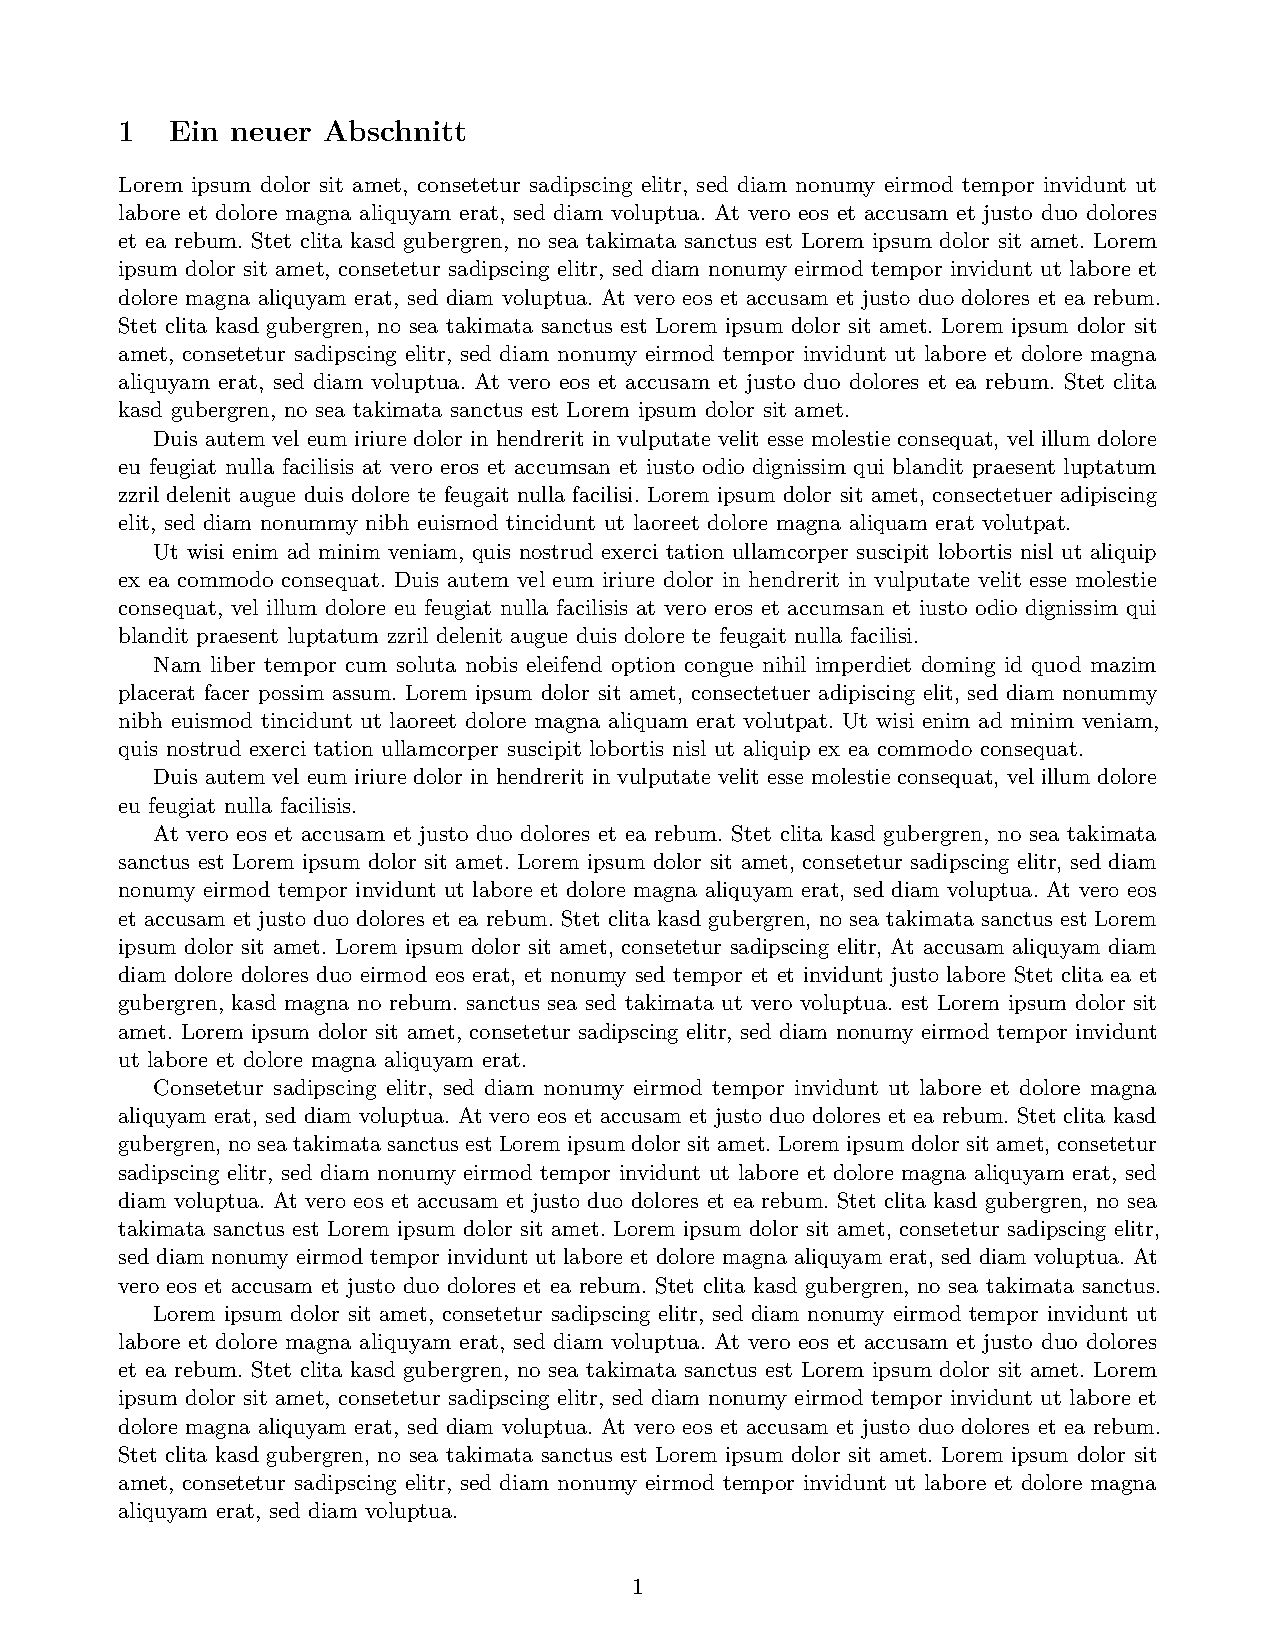
\includegraphics[scale=.23]{Beispiele/Zeilenabstand/Zeilenabstand_normal.pdf}}
\vspace{-5pt}
\caption{einfacher Zeilenabstand}
\end{figure}
\end{minipage}
\pause
\begin{minipage}{.49\textwidth}
\begin{figure}[htp]
\centering
\fbox{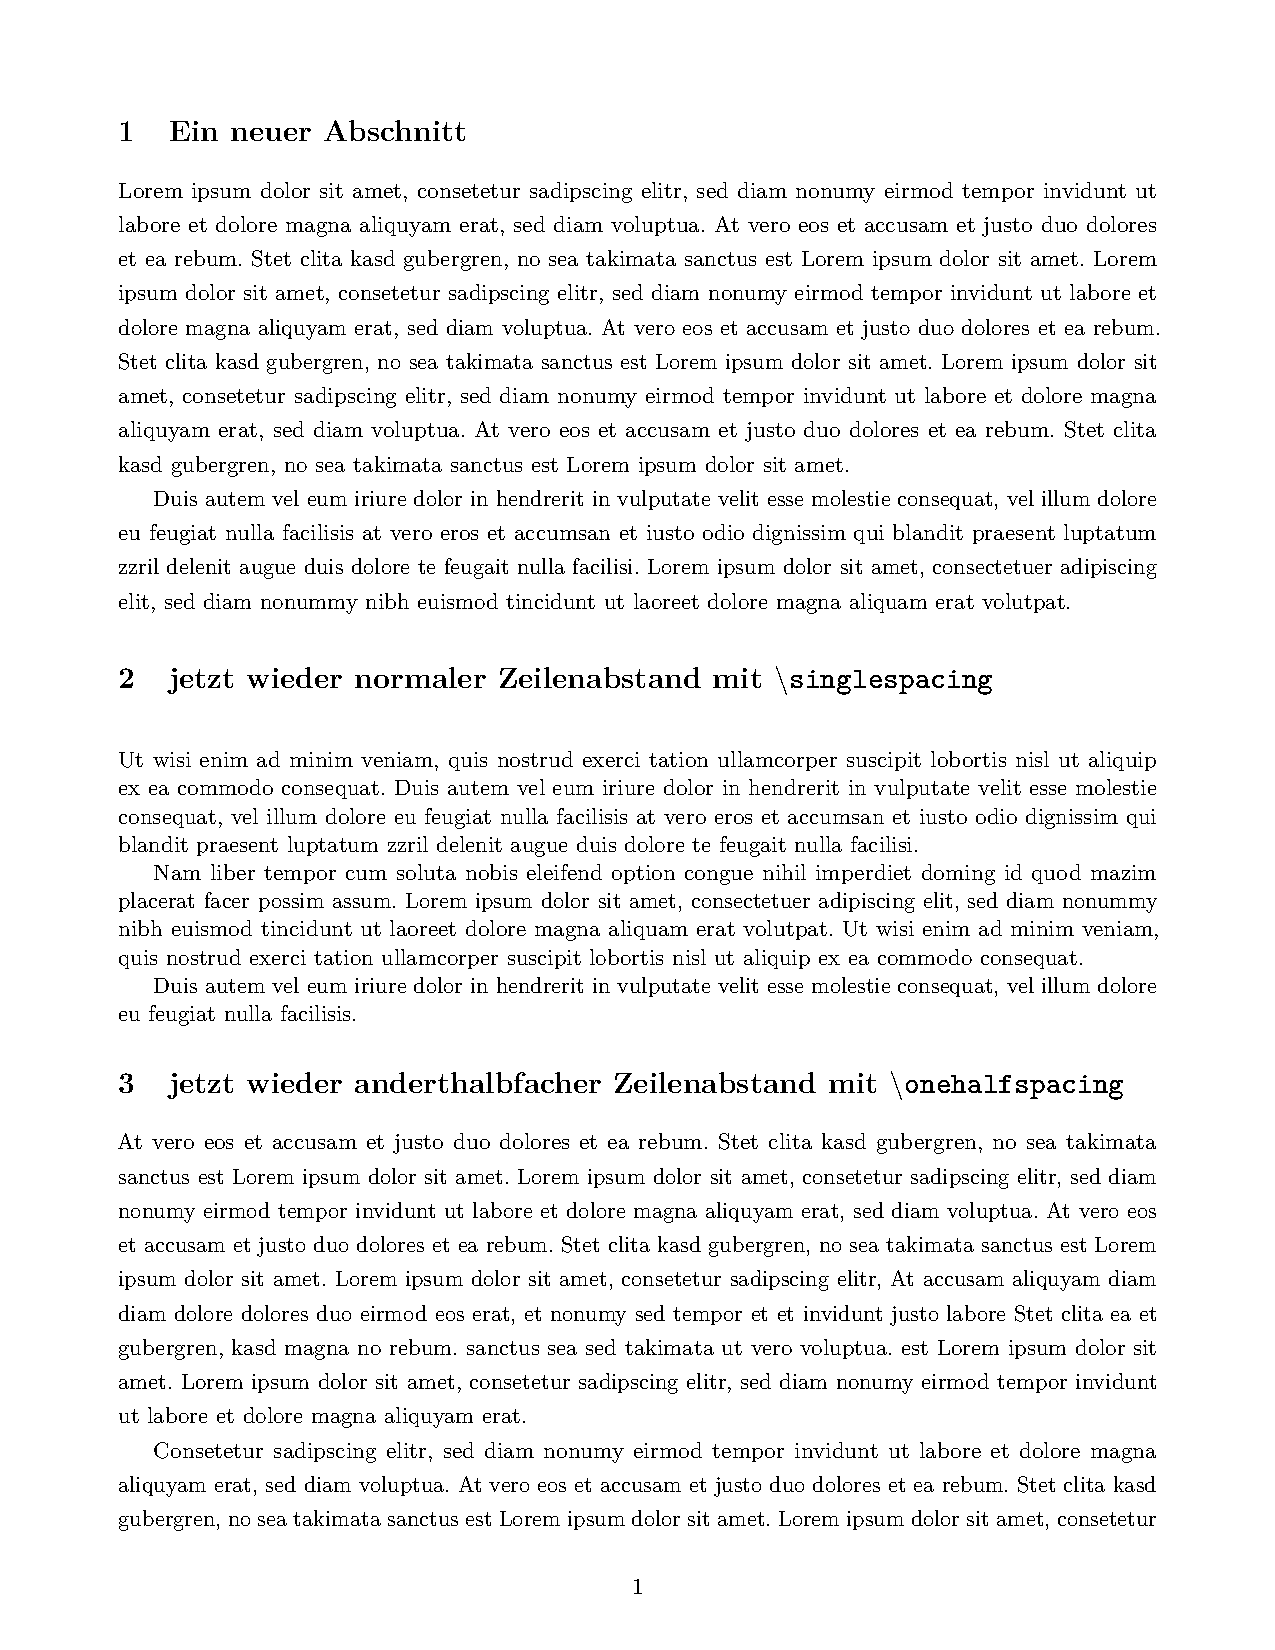
\includegraphics[scale=.23]{Beispiele/Zeilenabstand/Zeilenabstand.pdf}}
\vspace{-5pt}
\caption{einfacher und anderthalbfacher Zeilenabstand}
\end{figure}
\end{minipage}
\end{minipage}
\end{frame}




\subsection{Sonderzeichen}

\begin{frame}[fragile]
\frametitle{Lokalisierung}
Bei der Erstellung deutscher Texte sind folgende Pakete hilfreich:
\begin{description}[<+->]
  \item[babel] zum Einstellen der Sprache. Benötigt für Deutsch den Parameter [ngerman]
    \begin{itemize}
      \item deutsche Anführungszeichen
      \item Automatische Texte werden deutsch (z.B. ``Inhaltsverzeichnis'')
      \item Generiert den Befehl ``\verb+"+'', der deutsche Sonderzeichen erzeugen kann
      \item erlaubt die Verwendung von \verb+\glqq+ und \verb+\grqq+ um Anführungszeichen zu erzeugen
    \end{itemize}
  \item[inputenc] Definiert die Kodierung der .tex-Datei, welche als optionaler Parameter angegeben wird:
    \begin{itemize}
      \item \emph{utf8}: Universeller Standard
     % \item \emph{latin1, applemac}: Frühere Windows / Linux Standards
    \end{itemize}
\end{description}  
\end{frame}



\begin{frame}[fragile]
\frametitle{Anführungszeichen}
Nach dem Einbinden des \texttt{babel}-Paketes stehen folgende Anführungszeichen zur Verfügung: \pause

\begin{itemize}[<+->]
\item Pfeile: \verb+">Hallo"<+ ">Hallo"<
\item Englisch: \verb+``Hallo''+ ``Hallo''
\item Deutsch: \verb+"`Hallo"'+ "`Hallo"' 
\item oder \verb+\glqq+ Hallo \verb+\grqq+ \glqq Hallo\grqq 
\end{itemize}
\end{frame}



\begin{frame}
\frametitle{Lokalisierung}
\begin{description}[<+->]
  \item[fontenc] Sorgt dafür, dass alle 256 Zeichen des europäischen Zeichensatzes dargestellt werden können. Benötigt für europäischen Zeichensatz den optionalen Parameter [T1].
  \item[lmodern] Sorgt für eine Darstellung von Umlauten als Umlaute im PDF-Text und nicht als ``Buchstabe mit Pünktchen darüber''.
\end{description}
\pause
%Pakete für weitere Sonderzeichen können der ``Comprehensive Symbol List'' entnommen werden:
%  \url{http://www.ctan.org/tex-archive/info/symbols/comprehensive/symbols-a4.pdf}\\
%  Dadurch lassen sich tolle Symbole wie diese erstellen: \copyright, \$, \maltese, \checkmark, \PHplumedHead, \BlackBishopOnWhite, \EUR
\end{frame}



\begin{frame}[fragile]
\frametitle{Beispiel eines deutschen Textes}
\begin{lstlisting}[style=Latex]
\documentclass{article}
\usepackage[ngerman]{babel}
\usepackage[utf8]{inputenc}
\usepackage[T1]{fontenc}
\usepackage{lmodern}
\begin{document}
"`Hol mit bitte die Rührschüssel"' sagte Peter.\\
``Sorry I dont speak German'' antwortete Samantha.
\end{document}
\end{lstlisting} \vspace{-20pt}
\pause
Ergibt:
\result{
"`Hol mit bitte die Rührschüssel"' sagte Peter.\\
``Sorry I dont speak German'' antwortete Samantha.
">Standardtext"<
}
\end{frame}

\begin{frame}[fragile]
\frametitle{Beispiel eines deutschen Textes}
\begin{lstlisting}[style=Latex]
\documentclass{article}
\usepackage[ngerman]{babel}
\usepackage[utf8]{inputenc}
\usepackage[T1]{fontenc}
\usepackage{lmodern}
\usepackage[left=2cm,right=2cm,top=2cm,bottom=2cm]{geometry}
\begin{document}
ä Ä ö Ö ü Ü\\
\end{document}
\end{lstlisting} \vspace{-20pt}
\pause
Ergibt:
\result{
ä Ä ö Ö ü Ü\\
}
\end{frame}



\subsection{Seitengröße}
\begin{frame}[fragile,t]
\frametitle{Seitengröße}
Die Papiergröße lässt sich sehr komfortabel mit dem Paket {\tt geometry} einstellen:\vfill
\begin{lstlisting}[style=Latex]
\usepackage[left=2cm,right=2cm,top=2cm,bottom=2cm]{geometry}
\end{lstlisting}
\end{frame}


\begin{frame}[fragile,t]
\frametitle{Beispiel}
\vspace{-10pt}
\begin{minipage}{\textwidth}
\begin{minipage}{.49\textwidth}
%\vspace{-70pt}
\begin{figure}[htp]
\centering
\fbox{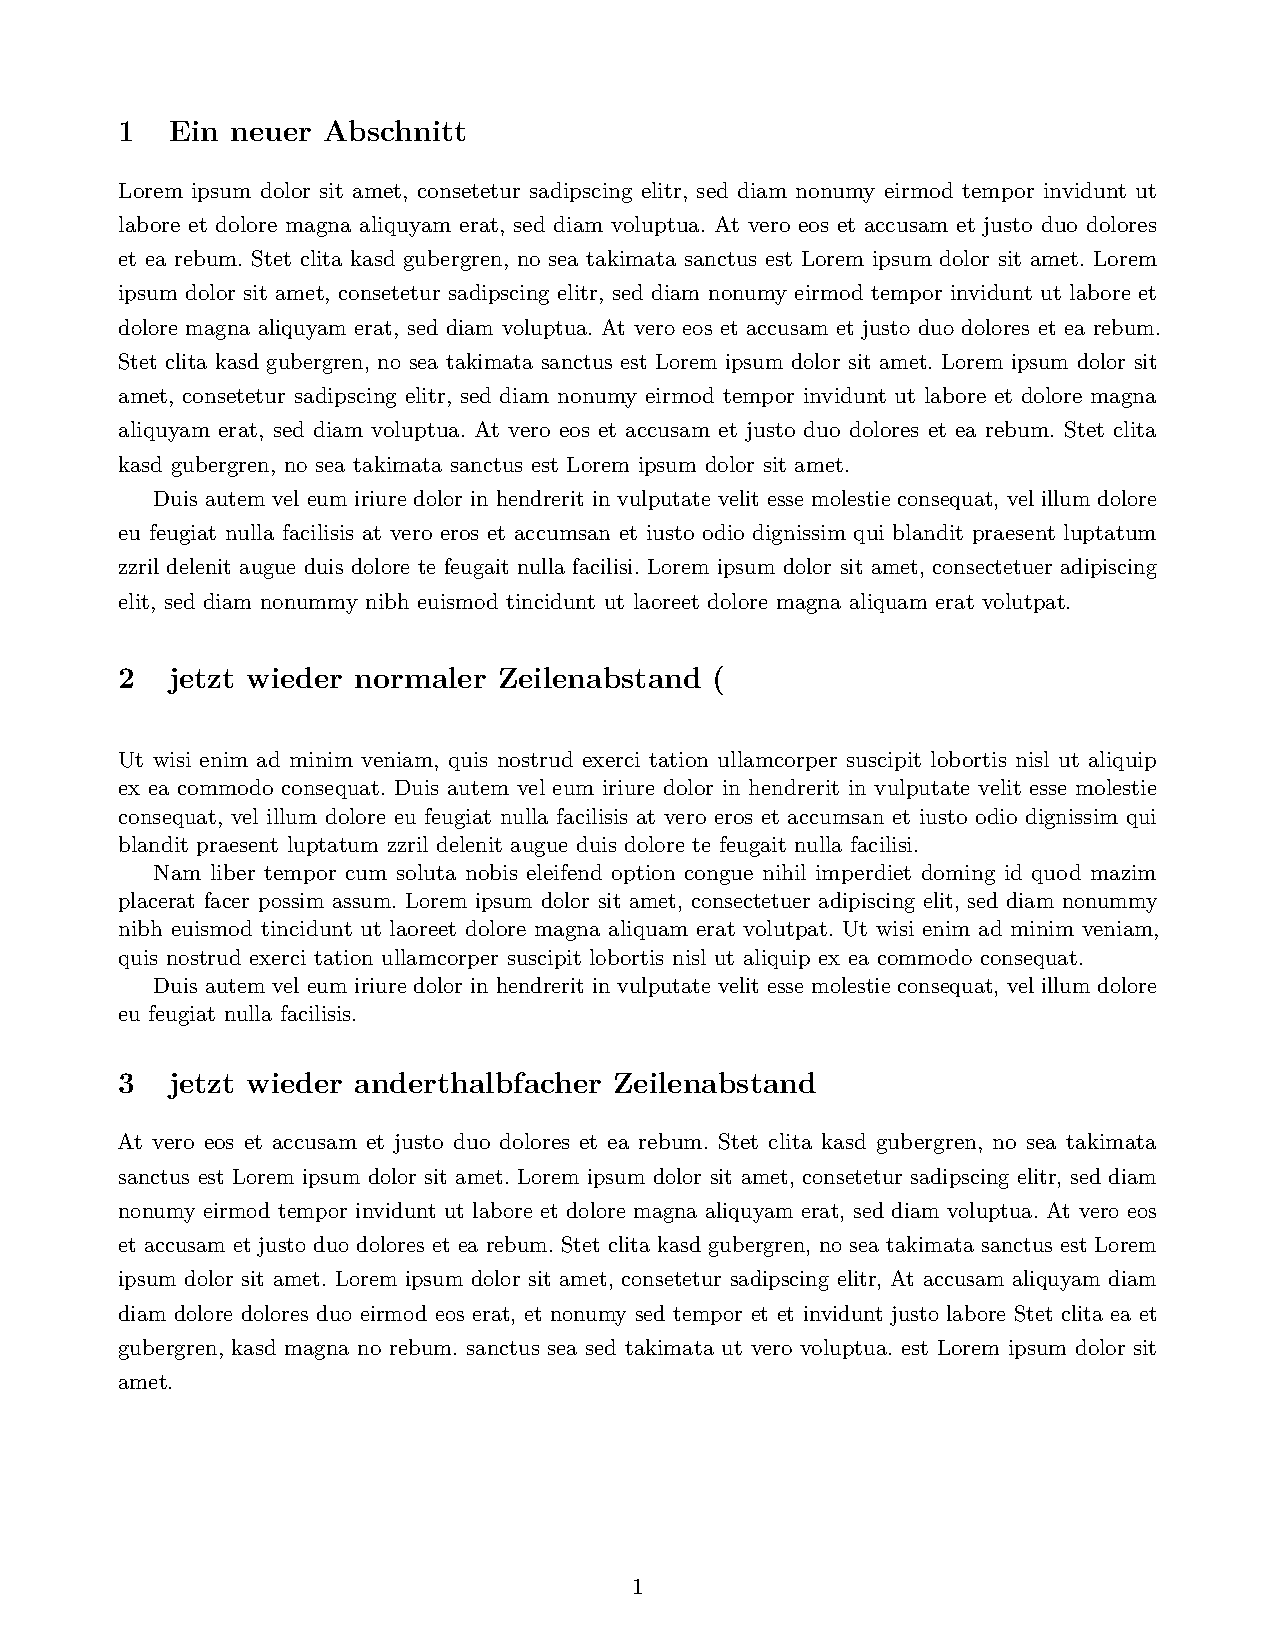
\includegraphics[scale=.23]{Beispiele/Rand/Zeilenabstand.pdf}}
\vspace{-5pt}
\caption{Überall 2cm Abstand zum Rand}
\end{figure}
\end{minipage}
\pause
\begin{minipage}{.49\textwidth}
\begin{figure}[htp]
\centering
\fbox{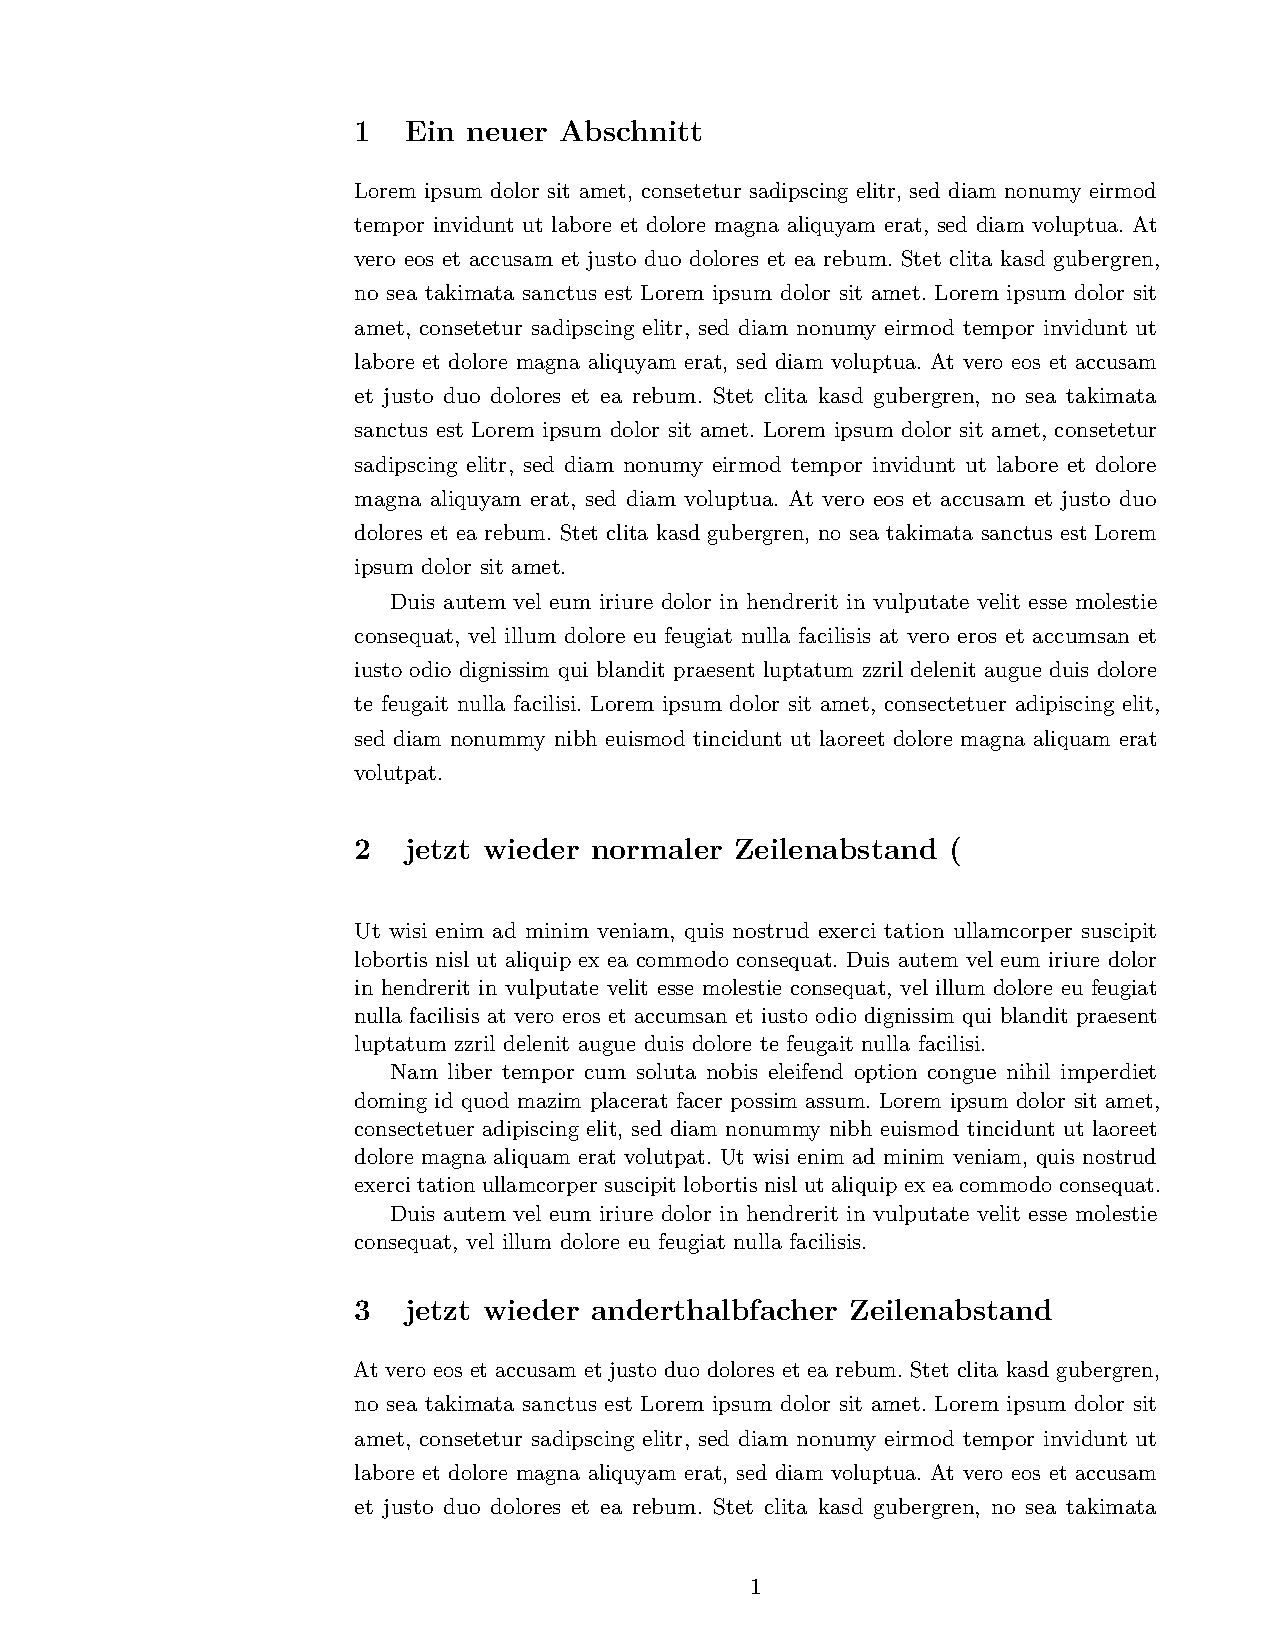
\includegraphics[scale=.23]{Beispiele/Rand/Zeilenabstand_normal.pdf}}
\vspace{-5pt}
\caption{links 6cm Abstand zum Rand}
\end{figure}
\end{minipage}
\end{minipage}
\end{frame}


\subsection{Seitenstile}


\begin{frame}[fragile,t]
\frametitle{Kopf- und Fußzeilen}
\begin{itemize}[<+->]
  \item Das Paket {\tt fancyhdr} ermöglicht eine einfache Verwendung von Kopf- und Fußzeilen
  \item Damit die Seiteneinstellungen korrekt übernommen werden sollten im Quellcode \textbf{zuerst} die Seitengröße durch das geometry-Paket eingestellt werden

  \item Aktivierung durch \begin{center}\lstinline[style=Latex]+\usepackage{fancyhdr}\pagestyle{fancy}+\end{center}
\item Die Syntax für mögliche Positionen lautet:\\
  \begin{center} \small
  \begin{tabular}{|c|} \hline
    \lstinline[style=Latex]+\lhead{<Inhalt>}+  \quad \lstinline[style=Latex]+\chead{<Inhalt>}+  \quad \lstinline[style=Latex]+\rhead{<Inhalt>}+  \\\hline\\
    \huge Text \\\\\hline
    \lstinline[style=Latex]+\lfoot{<Inhalt>}+ \quad \lstinline[style=Latex]+\cfoot{<Inhalt>}+ \quad \lstinline[style=Latex]+\rfoot{<Inhalt>}+ \\\hline
  \end{tabular}
  \end{center}
\end{itemize}
\end{frame}


\begin{frame}[fragile]
\frametitle{Beispiel Kopf und Fußzeile}
\begin{minipage}{.6\textwidth}
{\scriptsize
\begin{lstlisting}[style=Latex]
\documentclass[a4paper]{article}
\usepackage[ngerman]{babel}
\usepackage[utf8]{inputenc}
\usepackage[T1]{fontenc}
\usepackage{lmodern}
\usepackage{fancyhdr}\pagestyle{fancy}
\lhead{Linke Kopfzeile}
\rhead{rechte Kopfzeile}
\lfoot{linke Fußzeile} 
\cfoot{}
\rfoot{Seitenzahl: \thepage}
\begin{document}
"`Hol mit bitte die Rührschüssel"' sagte Peter.\\
``Sorry I dont speak German'' antwortete Samantha.
\end{document}
\end{lstlisting}}

\end{minipage}
\pause
\begin{minipage}{.39\textwidth}

\begin{figure}[htp]
\centering
\fbox{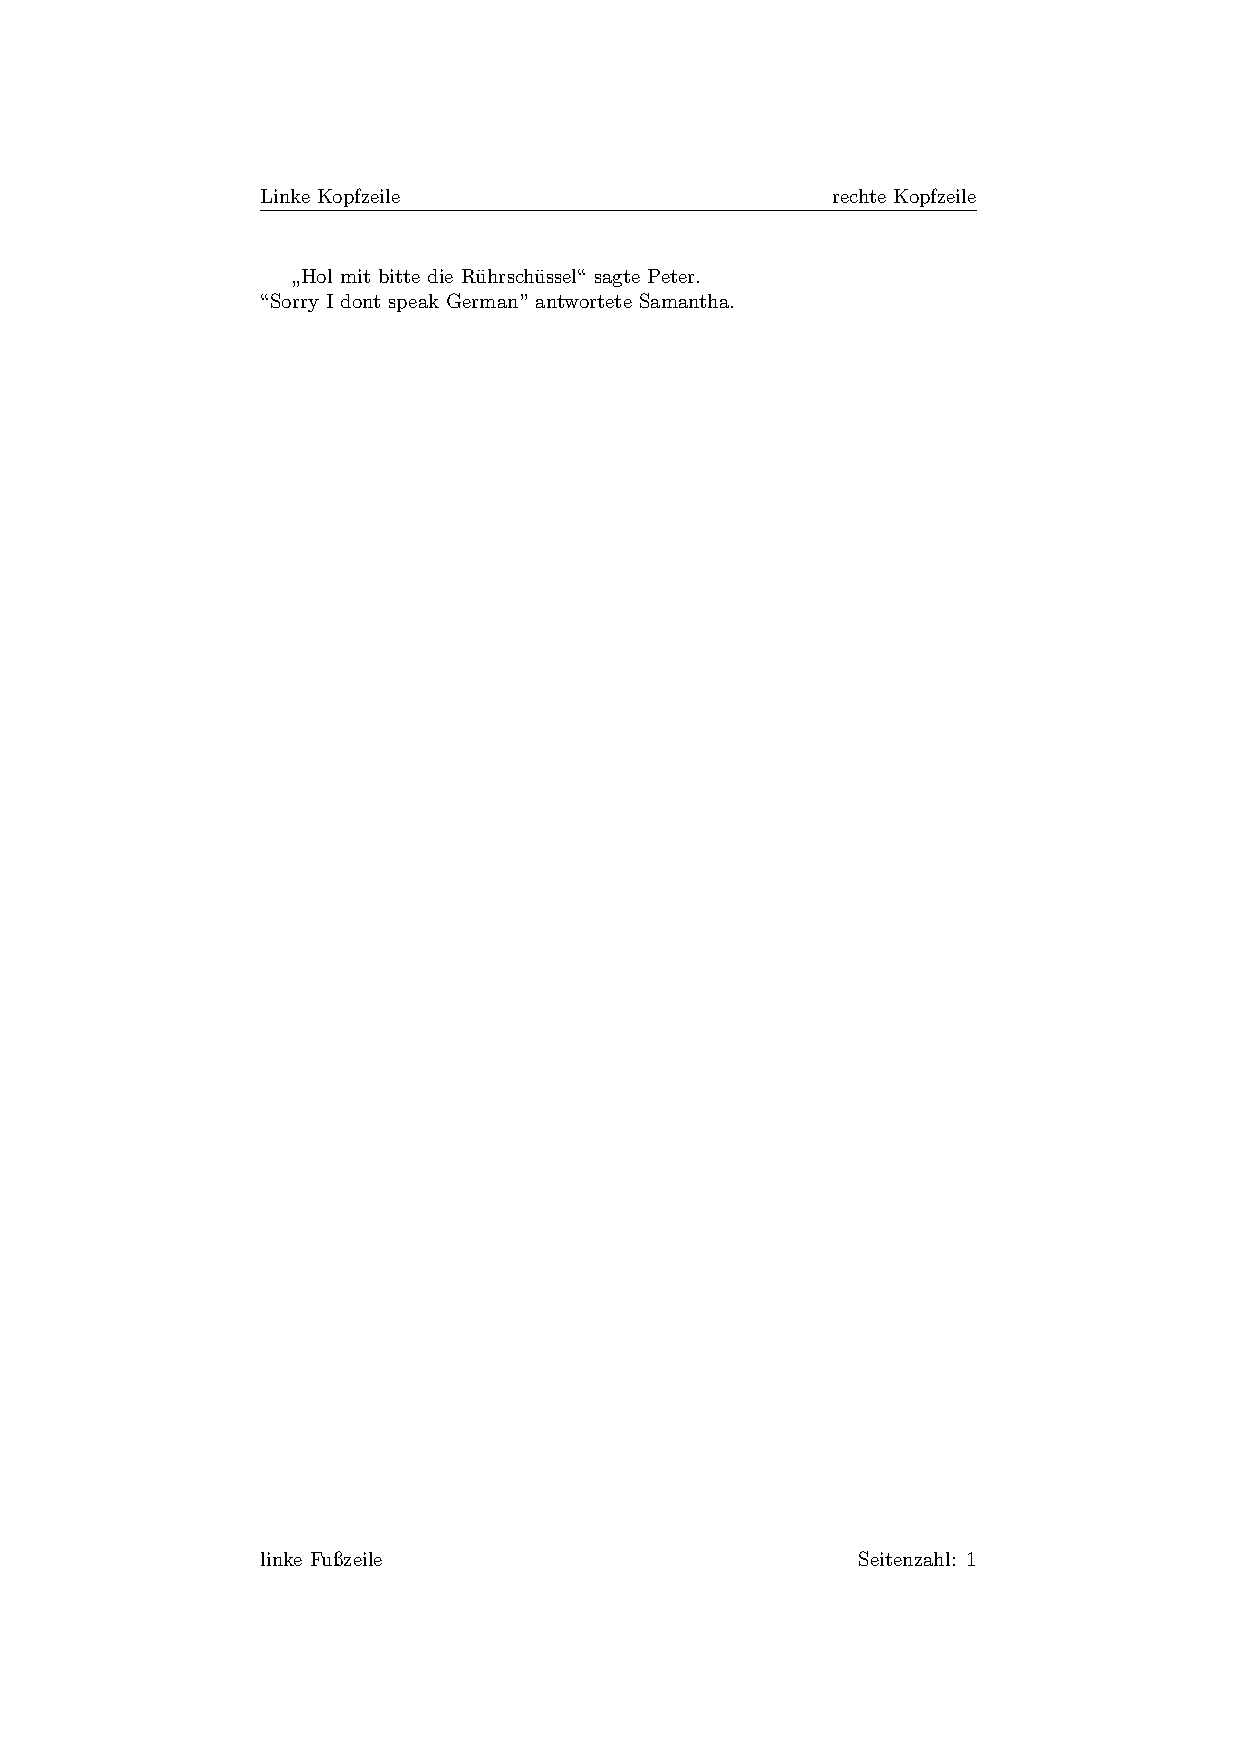
\includegraphics[scale=.25]{Beispiele/KopfundFusszeile/KopfundFusszeile.pdf}}
\vspace{-20pt}
\caption{Kopf- und Fußzeile}
\end{figure}

\end{minipage}
\end{frame}



\begin{frame}[fragile]
\frametitle{Verwendung von Zählern}
Anzeigen von bestimmten Elementen in Kopf- oder Fußzeile:
\begin{itemize}[<+->]
  	\item Kapitel (\lstinline[style=Latex]+\section+)	
	\item Unterkapitel (\lstinline[style=Latex]+\subsection+) , Unterunterkapitel (\lstinline[style=Latex]+\subsubsection+)
	\item Seitenanzahl (\lstinline[style=Latex]+\thepage+)
	\item Datum der Kompilierung (\lstinline[style=Latex]+\today+)
\end{itemize}
\end{frame}

\begin{frame}[fragile]
\frametitle{Seitennummerierung}
\begin{itemize}[<+->]
  \item Die Seitennummerierung wird festgelegt mit \\
  \quad \lstinline[style=Latex]+\pagenumbering{<Stil>}+
  \item Mögliche Stile sind
  \begin{itemize}
    \item \texttt{\textbf{arabic}}: Arabische Zahlen (Standard)
    \item \texttt{\textbf{roman}}/\texttt{\textbf{Roman}}: kleine/große römische Ziffern
    \item \texttt{\textbf{alph}}/\texttt{\textbf{Alph}}: Kleinbuchstaben/Großbuchstaben
  \end{itemize}
  \item Dies kann an jeder Stelle im Text geändert werden. Dabei wird jedoch der Zähler auf 1 gesetzt.
  \item Ändern des Zählers durch \lstinline[style=Latex]+\setcounter{page}{<Seitennummer>}+
\end{itemize}
\end{frame}

\subsection{Schriftbild}



\begin{frame}[fragile,t]
\frametitle{Schriftsatz}
Die Schrift in einer Umgebung <Text> lässt sich wie folgt anpassen:
\begin{itemize}[<+->]
  \item Schriftart
  \begin{itemize}
    \item \lstinline[style=Latex]+\textrm{<Text>}+: {\rmfamily Roman-Schrift}
    \item \lstinline[style=Latex]+\texttt{<Text>}+: {\ttfamily Schreibmaschinenschrift}
   % \item \lstinline[style=Latex]+\sf{<Text>}+: {\sffamily Serifenlose Schrift}
  \end{itemize}  
  \item Form:
  \begin{itemize}
    \item \lstinline[style=Latex]+\textit{<Text>}+: {\itshape Kursivschrift}
   % \item \lstinline[style=Latex]+\slshape+: {\slshape Geneigte Schrift}
   % \item \lstinline[style=Latex]+\scshape+: {\scshape Kapitälchen}
   % \item \lstinline[style=Latex]+\upshape+: {\upshape Aufrechte Schrift }
  \end{itemize}
  \item Serie:
  \begin{itemize}
    \item {\lstinline[style=Latex]+\textbf{<Text>}+: \bfseries Fettschrift}
   % \item \lstinline[style=Latex]+\mdseries+: {\mdseries Standard}
  \end{itemize}
\end{itemize}~\\
\pause
{\scriptsize
\begin{minipage}{.55\textwidth}
\begin{lstlisting}[style=Latex]
\texttt{Schreibmaschinenschrift}\\
\texttt{Schreib\textbf{maschinen}schrift}\\
\texttt{kursive Schrift}
\end{lstlisting}
\end{minipage}}\pause~
\begin{minipage}{.39\textwidth}
\result{
\texttt{Schreibmaschinenschrift}\\
\texttt{Schreib\textbf{maschinen}schrift}\\
\texttt{kursive Schrift}
}
\end{minipage}

\end{frame}


\begin{comment}
\begin{frame}[fragile]
\frametitle{Schriftsatz}
\begin{itemize}[<+->]
  \item Möchte man nicht die gesamte Umgebung ändern, sondern nur ein Wort o.ä., so bietet sich
\begin{lstlisting}[style=Latex] 
\text<Kuerzel>{<Text>} 
\end{lstlisting}\vspace{-20pt}
an. Als Kürzel gelten die ersten beiden Buchstaben der oben genannten Befehle (rm, it, up, ...).
\end{itemize}
\pause
\begin{lstlisting}[style=Latex]
{\ttfamily In einer Umgebung} \\
\texttt{So gehts auch} \\
\texttt{\sffamily Was passiert wohl hier?}
\end{lstlisting}\vspace{-20pt}
\pause
\result{
{\ttfamily In einer Umgebung} \\
\texttt{So gehts auch} \\
\texttt{\sffamily Was passiert wohl hier?}}
\end{frame}
\end{comment}

\begin{frame}[fragile]
\frametitle{Schriftsatz}
\begin{itemize}[<+->]
  \item Schriftgröße:
  \begin{center}\begin{tabular}{ll}
    				\lstinline[style=Latex]+\tiny+: 			& \tiny winzig\\
    \onslide<2->	\lstinline[style=Latex]+\scriptsize+:		& \onslide<2-> \scriptsize sehr klein\\
    \onslide<3->	\lstinline[style=Latex]+\footnotesize+:	& \onslide<3-> \footnotesize Fußnote\\
    \onslide<4-> \lstinline[style=Latex]+\small+:			& \onslide<4-> \small klein\\
    \onslide<5-> \lstinline[style=Latex]+\normalsize+:		& \onslide<5-> \normalsize normal\\
    \onslide<6-> \lstinline[style=Latex]+\large+:			& \onslide<6-> \large groß\\
    \onslide<7-> \lstinline[style=Latex]+\Large+:			& \onslide<7-> \Large Größer\\
    \onslide<8-> \lstinline[style=Latex]+\LARGE+:			& \onslide<8-> \LARGE sehr groß\\
    \onslide<9-> \lstinline[style=Latex]+\huge+:			& \onslide<9-> \huge riesig\\
    \onslide<10-> \lstinline[style=Latex]+\Huge+:			& \onslide<10-> \Huge gigantisch
  \end{tabular}\end{center}
 % \item<11-> Eigene Schriftgröße: \lstinline[style=Latex]+\fontsize{<size>}{<skip>}\selectfont+\\
  %  Dabei ist \lstinline[style=Latex]+<size>+ die Schriftgröße und \lstinline[style=Latex]+<skip>+ der Zeilenabstand in pt.
\end{itemize}
\end{frame}



\begin{frame}[fragile]
  \frametitle{Beispiel}
  \begin{lstlisting}[style=Latex]
\textbf{\large{ Es ist schwer, Internetzitate auf Echtheit zu testen}} \\
\scriptsize{\texttt{Abraham Lincoln}}
\end{lstlisting}
      \textbf{\large{ Es ist schwer, Internetzitate auf Echtheit zu testen}} \\
      \scriptsize{\texttt{Abraham Lincoln}}
\end{frame}

\begin{comment}
\begin{frame}[fragile]
  \frametitle{Farben}
  \begin{itemize}[<+->]
  \item Das \texttt{color}-Paket erlaubt die Benutzung von Farben in \LaTeX
  \item Definiert werden Farben mittels 
    \begin{center} \lstinline[style=Latex]+\definecolor{<Name>}{<System>}{<Spezifikation>}+ \end{center} \pause
    Systeme:
    \begin{itemize}
    \item \texttt{rgb} für RGB-Farben
    \item \texttt{gray} für Grautöne
    \item weitere Spezialsysteme, z.B. \texttt{html, cmyk}
    \end{itemize}
  \item Vordefiniert sind die Farben \textbf{black, white, red, green, blue, cyan, magenta, yellow}
  \item Außerdem sind nun verfügbar:
    \begin{itemize}
    \item \lstinline[style=Latex]+\textcolor{<Farbe>}{<Text>}+ färbt den eingefügten Text
    \item \lstinline[style=Latex]+\color{<Farbe>}+ färbt allen Text in der aktuellen Umgebung
    \item \lstinline[style=Latex]+\pagecolor{<Farbe>}+ färbt den Hintergrund der aktuellen Seite
    \item \lstinline[style=Latex]+\colorbox{<Farbe>}{<Text>}+ färbt den Hintergrund des Textes
    \item \lstinline[style=Latex]+\fcolorbox{<Farbe1>}{<Farbe2>}{<Text>}+ umrandet den Text mit Farbe1 und hinterlegt ihn mit Farbe2      
    \end{itemize}
  \end{itemize}
\end{frame}

\begin{frame}[fragile,t]
  \frametitle{Beispiel}
  \begin{lstlisting}[style=Latex]
    \definecolor{darkblue}{rgb}{0,0,.5}
    \definecolor{mygray}{gray}{.75}
    \textcolor{darkblue}{Hallo }
    \colorbox{mygray}{Welt}
  \end{lstlisting}
  \pause
  \vspace{-20pt}
\result{
  \definecolor{darkblue}{rgb}{0,0,.5}
  \definecolor{mygray}{gray}{.75}
  \textcolor{darkblue}{Hallo }
  \colorbox{mygray}{Welt}}
\end{frame}
\end{comment}



\subsection{Whitespaces}

\begin{frame}[fragile]
\frametitle{Zeilenumbrüche}
\begin{itemize}[<+->]
  \item ein Zeilenumbruch wird mittels \lstinline[style=Latex]+\\+ bzw. \lstinline[style=Latex]+\newline+ erzeugt.
  \item \lstinline[style=Latex]+\\+ kann als optionalen Parameter einen Abstand zur nächsten Zeile haben:\\
    \lstinline[style=Latex]+\\[5cm]+
 % \item \lstinline[style=Latex]+\linebreak[<Dringlichkeit>]+ erzeugt einen Zeilenumbruch, bei dem die aktuelle Zeile noch aufgefüllt wird.\\
 % Diese Dringlichkeit ist ein Wert zwischen 0 und 4.
  \item Zeilenumbrüche funktionieren nur nach Text, nach einer Umgebung muss unter Umständen ein Abstand (Tilde) eingefügt werden.
\end{itemize}
\end{frame}

\begin{frame}[fragile]
\frametitle{Absätze}
\begin{itemize}[<+->]
  \item Ein neuer Absatz wird durch eine Leerzeile erzeugt:
  \item neue Absätze werden standardmäßig eingerückt. Dieser Abstand wird mit \lstinline[style=Latex]+\parindent+ definiert.
  \item \lstinline[style=Latex]+\indent+ bzw. \lstinline[style=Latex]+\noindent+ fügen manuell diesen Abstand ein oder verhindern ihn für den aktuellen Absatz.
  \item Um die Einrückung im Dokument zu deaktivieren reicht es nach \lstinline[style=Latex]+\begin{document}+
\begin{center}
    \lstinline[style=Latex]+\setlength{\parindent}{0cm}+ 
\end{center}
zu schreiben
\end{itemize}
\end{frame}

\begin{comment}
\begin{frame}[fragile]
\frametitle{horizontaler Abstand}
\begin{itemize}[<+->]
  \item \lstinline[style=Latex]+\hspace{<Abstand>}+ erzeugt einen horizontalen Abstand.
  \item Beispiele: \\
    \lstinline[style=Latex]+Hallo \hspace{3ex} Welt+: Hallo \hspace{3ex} Welt\\
    \lstinline[style=Latex]+Hallo \hspace{-3ex} Welt+: Hallo \hspace{-3ex} Welt\\
  \item definierte Abstände sind (jeweils in Geviert)\\[1ex]
    \hspace{-3ex}\begin{tabular}{l||c|c|c|c|c|c}
    Befehl & \lstinline[style=Latex]+\!+ & \lstinline[style=Latex]+\,+ & \lstinline[style=Latex]+\;+ & \lstinline[style=Latex]+\ + & \lstinline[style=Latex]+\quad+ & \lstinline[style=Latex]+\qquad+ \\\hline
    Abstand & -3/18 & 3/18 & 5/18 & 1/3 & 1 & 2
    \end{tabular}
  \item \lstinline[style=Latex]+\hfill+ füllt so, dass der restliche Text rechtsbündig abschließt. Mehrere Aufrufe in einer Zeile ``teilen'' sich den Rest. Ebenso \lstinline[style=Latex]+\dotfill+ und \lstinline[style=Latex]+\hrulefill+.
\noindent
\begin{lstlisting}[frame=single]
T1 \hfill T2 \dotfill T3 \hrulefill T4
\end{lstlisting} 
\pause
\vspace{-20pt}
\result{ 
    T1 \hfill T2 \dotfill T3 \hrulefill T4}
\end{itemize}
\end{frame}
\end{comment}

\begin{frame}[fragile]
\frametitle{vertikaler Abstand}
\begin{itemize}[<+->]
  \item Füllen des Rests der Seite mit Leerzeilen
  \begin{itemize}
     % \item \lstinline[style=Latex]+\pagebreak+: wie \lstinline[style=Latex]+\linebreak+
     % \item \lstinline[style=Latex]+\vspace+: wie \lstinline[style=Latex]+\hspace+
      \item \lstinline[style=Latex]+\vfill+%wie \lstinline[style=Latex]+\hfill+
    \end{itemize}\vfill
  \item Erstellen einer neuen Seite:
    \begin{itemize}
      \item \lstinline[style=Latex]+\newpage+%: Erzeugt eine neue Seite% wie \lstinline[style=Latex]+\newline+
     % \item \lstinline[style=Latex]+\pagebreak+: wie \lstinline[style=Latex]+\linebreak+
     % \item \lstinline[style=Latex]+\vspace+: wie \lstinline[style=Latex]+\hspace+
     % \item \lstinline[style=Latex]+\vfill+: wie \lstinline[style=Latex]+\hfill+
    \end{itemize}\vfill
  \item definierte Abstände nach Absätzen: \\
    \lstinline[style=Latex]+\bigskip+\hfill \lstinline[style=Latex]+\medskip+\hfill \lstinline[style=Latex]+\smallskip+ \hfill\,
\vfill
  \item Abstand nach einem Zeilenumbruch durch:\\
    \lstinline[style=Latex]+\\[2cm]+
\end{itemize}
\end{frame}

\subsection{Positionierung}

\begin{frame}[fragile]
\frametitle{Positionierung}
\begin{itemize}[<+->]
\item die \texttt{center}-Umgebung ist direkt von sich aus zentriert
\item analog dazu existiert die \texttt{flushright}- bzw. \texttt{flushleft}-Umgebung
\end{itemize}
\end{frame}

\begin{frame}[fragile,t]
  \frametitle{Beispiel}
  \begin{lstlisting}[style=Latex]
\begin{center}
Dieser Text ist zentriert,
\end{center}
\begin{flushright}
dieser hier nach rechts ausgerichtet.
\end{flushright}
\end{lstlisting}\vspace{-20pt}
  \pause
\result{
  \begin{center}
    Dieser Text ist zentriert,
  \end{center}
  \begin{flushright}
    dieser hier nach rechts ausgerichtet.
  \end{flushright}}
\end{frame}

\subsection{Gliederung}


\begin{frame}[fragile]
\frametitle{Gliederungsebenen}
\begin{itemize}[<+->]
  \item Syntax: \lstinline[style=Latex]+\<Ebene>[<Kurzform>]{<Titel>}+
  \item Mögliche Ebenen sind:
  \begin{itemize}
    \item part: Teil (nur bei book)
    \item chapter: Kapitel (nur bei book und report)
    \item section: Abschnitt
    \item subsection: Unterabschnitt
    \item subsubsection: Unterunterabschnitt
    \item paragraph: Absatz
    \item subparagraph: Unterabsatz
  \end{itemize}
  \item Der optionale Parameter <Kurzform> taucht als Name im Inhaltsverzeichnis und im Header auf.
  \item Die Nummerierung kann mit ``*'' unterdrückt werden: \lstinline[style=Latex]+\section*{Nummerlos}+
\end{itemize}
\end{frame}

%\begin{frame}[fragile,t]
\frametitle{Übersicht}
\tableofcontents
\end{frame}
\section{Tabellen, Listen, Boxen}
\subsection{Tabellen}

\begin{frame}[fragile]
\frametitle{tabular}
\begin{itemize}[<+->]
  \item Tabellen werden mit der \texttt{tabular}-Umgebung erzeugt. Die Syntax ist 
    \begin{lstlisting}[style=Latex]
\begin{tabular}[Position]{<Spaltenformatierung>}
<Inhalt>
\end{tabular}
\end{lstlisting}\vspace{-20pt}
  \item gültige \texttt{<Position>} Parameter sind
  \begin{itemize}
    \item \texttt{l,r,c}: linksbündige / rechtsbündige / zentrierte Spalte
  \end{itemize}
  \item mit einem \lstinline[style=Latex]+&+ nächste Spalte
  \item mit einem \lstinline[style=Latex]+\\+ nächste Zeile
  \item horizontale Linien werden erzeugt durch:
  \begin{itemize}
    \item \lstinline[style=Latex]|\hline| Linie über die gesamte Breite
  \end{itemize}
\end{itemize}
\end{frame}


\begin{frame}[fragile,t]
\frametitle{Beispiel}
\begin{lstlisting}[style=Latex]
\begin{tabular}{r|c||l|}
rechts & zentriert & links \\ \hline
wieder & alles & normal
\end{tabular}
\end{lstlisting}
\pause\vspace{-20pt}
\result{
\begin{tabular}{r|c||l|}
rechts & zentriert & links \\ \hline
wieder & alles & normal\\
\end{tabular}}
\end{frame}

\begin{frame}[fragile,t]
\frametitle{Noch zu Tabellen}
Tabellen lassen sich jedoch noch leichter durch Onlinetools wie
\begin{center}
\url{http://www.tablesgenerator.com/}
\end{center}
erstellen.

\begin{figure}[htp]
\centering
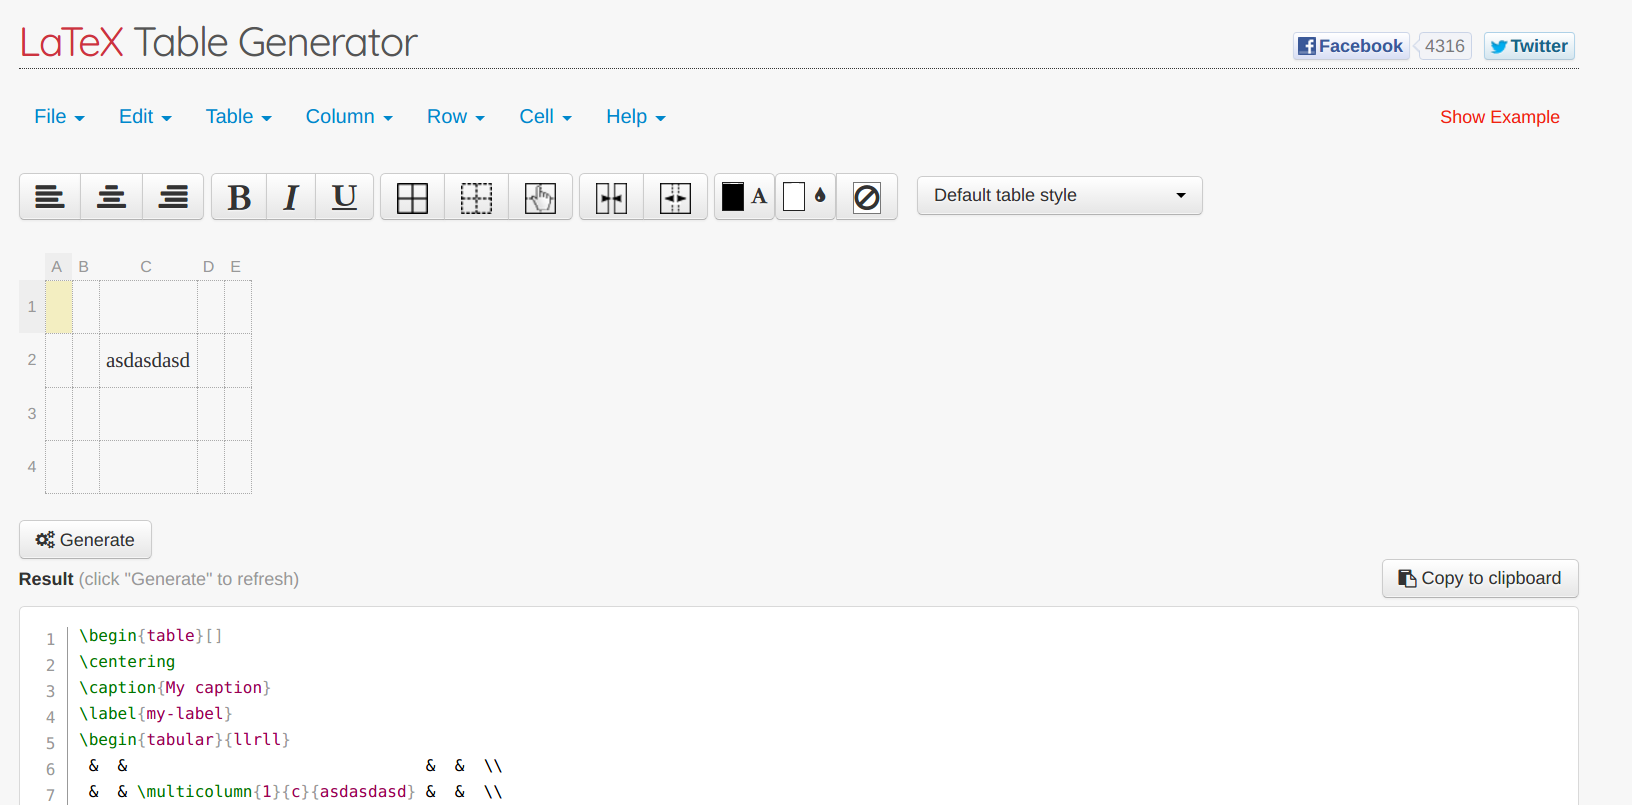
\includegraphics[scale=0.18]{images/onlinetable.png}
\end{figure}
\end{frame}



\subsection{Listen}

\begin{frame}[fragile]
\frametitle{Listen}
\begin{itemize}[<+->]
  \item Listen werden durch die \texttt{itemize}-Umgebung erzeugt.
  \item durch \lstinline[style=Latex]+\item+ wird ein Aufzählungspunkt erzeugt. Als optionaler Parameter kann das Aufzählungszeichen angegeben werden.
\end{itemize}
\end{frame}

\begin{frame}[fragile,t]
\frametitle{Beispiel 1}\vspace{-10pt}
\begin{lstlisting}[style=Latex]
\begin{itemize}
  \item Punkt 1
  \begin{itemize}
    \item Unterpunkt 1
    \item Unterpunkt 2
  \end{itemize}
  \item[*] Punkt 2
  \item Punkt 3
\end{itemize}
\end{lstlisting}
\pause\vspace{-25pt}
\result{\vspace{-10pt}
\begin{itemize}
  \item Punkt 1
  \begin{itemize}
    \item Unterpunkt 1
    \item Unterpunkt 2
  \end{itemize}
  \item[*] Punkt 2
  \item Punkt 3
\end{itemize}\vspace{-10pt}}
\end{frame}
\begin{frame}[fragile]
\frametitle{Listen}
Aufzählungen werden analog durch \texttt{enumerate} erzeugt.
\end{frame}
\begin{frame}[fragile,t]
\frametitle{Beispiel 2}\vspace{-10pt}
\begin{lstlisting}[style=Latex]
\begin{enumerate}
  \item Punkt 1
  \begin{enumerate}
    \item Unterpunkt 1
    \item Unterpunkt 2
  \end{enumerate}
  \item Punkt 2
  \item Punkt 3
\end{enumerate}
\end{lstlisting} 
\pause\vspace{-25pt}
\result{\vspace{-10pt}
\begin{enumerate}
  \item Punkt 1
  \begin{enumerate}
    \item Unterpunkt 1
    \item Unterpunkt 2
  \end{enumerate}
  \item Punkt 2
  \item Punkt 3
\end{enumerate}\vspace{-10pt}}
\end{frame}
\begin{frame}[fragile]
\frametitle{Listen}
Mithilfe des Pakets \texttt{enumerate} können die Aufzählungszeichen leicht geändert werden.
\end{frame}
\begin{frame}[fragile,t]
\frametitle{Beispiel 3}\vspace{-10pt}
\begin{lstlisting}[style=Latex]
\begin{enumerate}[(i)]
  \item Punkt 1
  \begin{enumerate}[a)]
    \item Unterpunkt 1
    \item Unterpunkt 2
  \end{enumerate}
  \item Punkt 2
  \item Punkt 3
\end{enumerate}
\end{lstlisting} 
\pause\vspace{-25pt}
\result{\vspace{-10pt}
\begin{enumerate}[(i)]
  \item Punkt 1
  \begin{enumerate}[a)]
    \item Unterpunkt 1
    \item Unterpunkt 2
  \end{enumerate}
  \item Punkt 2
  \item Punkt 3
\end{enumerate}\vspace{-10pt}}
\end{frame}
\begin{frame}[fragile]
\frametitle{Listen}
 Aufzählungen mit Namen für jeden Punkt werden durch \texttt{description} erzeugt.
\begin{itemize}[<+->]
  \item das Aussehen dieser Listen variiert je nach Dokumentenklasse!
  \item durch Ändern der Variablen \lstinline[style=Latex]+\labelitemi+, \lstinline[style=Latex]+\labelitemii+, etc können die Aufzählungssymbole global geändert werden.
\end{itemize}
\end{frame}
\begin{frame}[fragile]
\frametitle{Beispiel 4}
\begin{lstlisting}[style=Latex]
\begin{description}
  \item[Label 1] Punkt 1
  \item[toller Name] Punkt 2
  \item[Bla] Punkt 3
\end{description}
\end{lstlisting} \vspace{-20pt}
\pause\result{
\begin{description}
  \item[Label 1] Punkt 1
  \item[toller Name] Punkt 2
  \item[Bla] Punkt 3
\end{description}}
\end{frame}
\begin{comment}
\subsection{Tabulatoren}


\begin{frame}[fragile]
\frametitle{tabulatoren}
\begin{itemize}[<+->]
  \item Tabulatoren können in der \texttt{tabbing}-Umgebung verwendet werden.
  \item Steuerzeichen sind:
  \begin{itemize}
    \item \lstinline[style=Latex]+\=+ neuer Tabulator
    \item \lstinline[style=Latex]+\\+ neue Zeile
    \item \lstinline[style=Latex]+\>+ nächster Tabulator
    \item \lstinline[style=Latex]+\<+ ein Tabulator zurück
    \item \lstinline[style=Latex]|\+| wie \lstinline[style=Latex]+\>+ nur über Zeilengrenzen hinweg
    \item \lstinline[style=Latex]+\-+ wie \lstinline[style=Latex]+\<+ nur über Zeilengrenzen hinweg
    \item \lstinline[style=Latex]+\'+ Tabsprung und zentriert den vorherigen Tab
    \item \lstinline[style=Latex]+\kill+ blendet die letzte Zeile aus (für Musterzeile)
  \end{itemize}
\end{itemize}
\end{frame}

\begin{frame}[fragile,t]
\frametitle{Beispiel}\vspace{-10pt}
\begin{lstlisting}[style=Latex]
\begin{tabbing}
 Breite 1 \= Breite 2 \= B3 \= Breite 4 \kill
 T1 \> T2 \> \> Tablulator 3 \+ \\
 A1 \> A2 \> A3 \\
 Text \= vieeeeeel zu lang \> Text 2 \\
 \> in neuen Tab \\
 \< wieder an Anfangstab 
\end{tabbing}
\end{lstlisting} 
\pause\vspace{-20pt}
\result{\vspace{-15pt}
\begin{tabbing}
 Breite 1 \= Breite 2 \= B3 \= Breite 4 \kill
 T1 \> T2 \> \> Tablulator 3 \+ \\
 A1 \> A2 \> A3 \\
 Text \= vieeeeeel zu lang \> Text 2 \\
 \> in neuen Tab \\
 \< wieder an Anfangstab 
\end{tabbing}\vspace{-15pt}}
\end{frame}
\end{comment}


\begin{comment}
\begin{frame}[fragile]
\frametitle{Boxen}
\begin{itemize}[<+->]
  \item In \LaTeX\, dienen Boxen dazu, den Inhalt als ein einzelnes Objekt zu betrachten. Dies hat mehrere Vorteile:
  \begin{itemize}
    \item die Box kann verschoben werden
    \item der Box können Grenzen angegeben werden
    \item sie kann eingerahmt werden
  \end{itemize}
  \item Syntax: \lstinline[style=Latex]+\makebox[<Breite>][<Pos>]{<Inhalt>}+
  \item als Position sind gültig:
  \begin{itemize}
    \item leer: zentriert
    \item \texttt{l}: linksbündig
    \item \texttt{r}: rechtsbündig
    \item \texttt{s}: gestreckt
  \end{itemize}
  \item automatische Breite: \lstinline[style=Latex]+\mbox+
  \item umrahmte Boxen: \lstinline[style=Latex]+\framebox+ bzw. \lstinline[style=Latex]+\fbox+.
\end{itemize}
\end{frame}

\begin{frame}[fragile]
\frametitle{raisebox}
\begin{itemize}[<+->]
  \item Boxen können verschoben werden mit
    \lstinline[style=Latex]+\raisebox{<Lift>}[<oben>][<unten>]{<Inhalt>}+
  \item dabei bedeuten
  \begin{itemize}
    \item \texttt{<Lift>}: soviel wird die Box angehoben
    \item \texttt{<oben>}: Abstand zur oberen Linie
    \item \texttt{<unten>}: Abstand zur unteren Linie
  \end{itemize}
\end{itemize}
\end{frame}
\end{comment}

\subsection{Minipage}

\begin{frame}[fragile]
\frametitle{minipage}
\begin{itemize}[<+->]
  \item Syntax: 
  \begin{lstlisting}[style=Latex]
\begin{minipage}[<Pos>]{<Breite>}
<Inhalt>
\end{minipage}
\end{lstlisting}\vspace{-20pt}
  \item \texttt{<Breite>} können in den bekannten Einheiten angegeben werden
  \begin{itemize}
    \item beachte die Verwendung von Konstanten wie \lstinline[style=Latex]+\textwidth+!
  \end{itemize}
  \item \texttt{<Pos>}: welche Zeile soll mit der aktuellen abschließen:
  \begin{itemize}
    \item \texttt{t}: oberste Zeile der Box
    \item \texttt{b}: unterste Zeile der Box
    \item nichts: Box wird zentriert
  \end{itemize}
%  \item \texttt{<iPos>}: Textanordnung innerhalb der Box:
%  \begin{itemize}
%    \item \texttt{t}: Text schließt oben ab
%    \item \texttt{b}: Text schließt unten ab
%    \item \texttt{c}: Text wird mittig zentriert
%    \item ohne: Text wird über die gesamge Höhe gestreckt
%  \end{itemize}
\end{itemize}
\end{frame}



\begin{frame}[fragile,t]
\frametitle{Beispiel}
\begin{lstlisting}[style=Latex]
\begin{minipage}{.49\textwidth}
Linke Minipage
\end{minipage}
\begin{minipage}{.49\textwidth}
Rechte Minipage
\end{minipage}
\end{lstlisting}\pause
\result{
\begin{minipage}{.49\textwidth}
Linke Minipage
\end{minipage}
\begin{minipage}{.49\textwidth}
Rechte Minipage
\end{minipage}}

\end{frame}

%\section{Bilder}
\shorthandoff{"}
\subsection{Bilddateien}

\begin{frame}[fragile]
\frametitle{Dateien einbinden}
\begin{itemize}[<+->]
  \item um externe Bilder in \LaTeX\ einzubetten muss in der Präambel das Paket \texttt{graphicx} durch \\
\begin{center}
\lstinline[style=Latex]+\usepackage{graphicx}+
\end{center}
eingebunden werden \vfill
  \item ein Bild wird mittels \lstinline[style=Latex]+\includegraphics[<Parameter>]{<Datei>}+ eingebunden. \\
Ein wichtiger Parameter ist
  \begin{itemize}
 %   \item \texttt{angle}: dreht das Bild um einen bestimmten Winkel
    \item \texttt{scale}: streckt das Bild um einen Faktor (beachte \lstinline[style=Latex]+\textwidth+)
 %   \item \texttt{height/width}: legt die Höhe/Breite fest
 %   \item \texttt{bb}: definiert die Grenzen der Bilddatei in vier Werten
 %   \item \texttt{clip}: wenn auf \texttt{true} gesetzt und zusammen mit \texttt{bb} verwendet, wird das Bild entsprechend zugeschnitten
  \end{itemize}
 % \item mit \lstinline[style=Latex]+\graphicspath{<Pfad>}+ kann angegeben werden, wo die Bilder liegen
 % \item über \lstinline[style=Latex]+\DeclareGraphicsExtensions{<Endungen>}+ kann definiert werden, nach welchen Bildern standardmäßig gesucht wird
\end{itemize}
\end{frame}

\begin{frame}[fragile]
\frametitle{figure-Umgebung}
\begin{itemize}[<+->]
  \item die \texttt{figure}-Umgebung ist eine Gleitbox für Bilder
  \item die Syntax ist
  \begin{lstlisting}[style=Latex]
\begin{figure}[<Pos>]
<Bild>
\end{figure}  
  \end{lstlisting}
  \item die Position wird angegeben durch verschiedene Buchstaben
  \begin{itemize}
    \item[h] das Bild wird auf der Momentanen Seite eingebunden
    \item[t/b] das Bild wird oben / unten auf der Seite eingebunden
    \item[p] das Bild kommt auf eine eigene Seite
  \end{itemize}
  \item zusätzlich ist der \lstinline[style=Latex]+\caption{<Text>}+-Befehl verfügbar, der dem Bild einen Untertitel verschafft
 % \item viele Bilder können mittels \lstinline[style=Latex]+\subfigure+ nebeneinander eingefügt werden
\end{itemize}
\end{frame}

   
\begin{frame}[fragile]
\frametitle{Beispiel}
\begin{lstlisting}[style=Latex]
\begin{figure}[h]
  
\includegraphics[width=.4\textwidth]{hypnotoad.png}
  \caption{all glory to the hypnotoad}
\end{figure}
\end{lstlisting} \vspace{-25pt}
\pause
\begin{figure}[h]
  
\includegraphics[width=.4\textwidth]{images/hypnotoad.png}
  \caption{all glory to the hypnotoad}
\end{figure}
\end{frame}

\begin{comment}
\subsection{TikZ}
\begin{frame}
\frametitle{TikZ}
\begin{itemize}[<+->]
  \item \textbf{T}ikZ \textbf{i}st \textbf{k}ein \textbf{Z}eichenprogramm
  \item Vektorgrafiken direkt in \LaTeX\, erstellen
  \item Vorteile:
  \begin{itemize}
    \item Alle Vorteile von \LaTeX
    \item fügt sich nahtlos ein
    \item ununterbrochener Workflow
    \item schnell
  \end{itemize}
  \item Nachteile:
  \begin{itemize}
    \item Ergebnis erst zum Schluss
    \item Einarbeitungszeit
  \end{itemize}
\end{itemize}
\end{frame}

\begin{frame}[fragile]
\frametitle{TikZ}
\begin{itemize}[<+->]
  \item TikZ wird mittels \lstinline[style=Latex]+\usepackage{tikz}+ geladen
  \item über \lstinline[style=Latex]+\usetikzlibrary{<library>}+ können zusätzliche Module geladen werden
  \item Nutzung über \lstinline[style=Latex]+\tikz{<Befehle>}+ oder die \texttt{tikzpicture}-Umgebung.
  \item Syntax: \lstinline[style=Latex]+\<Befehl>[<Parameter>](<Koordinate>){<Objekte>};+ 
  \item bei Verschachtelung mehrerer Befehle erhält nur der erste Befehl einen \lstinline[style=Latex]+\+: \\
  	\lstinline[style=Latex]+\draw (0,0) -- coordinate (b) (1,1);+  	
\end{itemize}
\end{frame}

\begin{frame}[fragile]
\frametitle{Koordinaten}
\begin{itemize}[<+->]
  \item Koordinaten können auf verschiedene Weisen angegeben werden:
  \begin{itemize}
    \item kartesisch: (X,Y)
    \item polar: ($\alpha$:r)
    \item Name: (Name)
  \end{itemize}
  \item Gültige Einheiten sind alle \TeX-Einheiten, Standard ist cm.
  \item Koordinaten können mittels 
  \begin{lstlisting}[style=Latex]
\coordinate (<Name>) at (<Position>);
  \end{lstlisting}
  gespeichert werden.
  \begin{itemize}
    \item steht \lstinline[style=Latex]+\coordinate+ direkt hinter einer Koordinate, so wird diese als Position übernommen
    \item steht \lstinline[style=Latex]+\coordinate+ direkt hinter einer Verbindungslinie (\lstinline[style=Latex]+--+), so wird die Mitte der Strecke zwischen den beiden Koordinaten übergeben
  \end{itemize}
\end{itemize}
\end{frame}

\begin{frame}[fragile]
\frametitle{Berechnungen}
\begin{itemize}[<+->]
  \item Nach dem Einbinden des Pakets \texttt{calc} kann man mit Koordinaten rechnen:
  \begin{itemize}
    \item Punkt auf einer Geraden: (\$(K1)!.3!(K2)\$)
    \item Addition: (\$(K1)+(K2)\$)
    \item Addition zur letzten: ++(K1)
  \end{itemize}
  \item noch komplexere Berechnungen funktionieren mittels \texttt{intersection}:\\
     \begin{lstlisting}[style=Latex]
(intersection cs: first line={(0,0)--(2,1)}, 
  second line={(0,1)--(2,-1)})
\end{lstlisting}
     berechnet den Schnittpunkt der Geraden durch (0,0)-(2,1) und (0,1)-(2,-1).
     \item TikZ kann noch viel mehr, mehr dazu in der Dokumentation
\end{itemize}
\end{frame}

\begin{frame}[fragile]
\frametitle{Beispiel}
\begin{lstlisting}[style=Latex]
\begin{tikzpicture}
\coordinate (a) at (0,0);
\coordinate (b) at (3,3);
\draw (a) -- (b) 
  -- ++ (-1,-2) coordinate (c) 
  -- ($(a)!.5!(b)$) coordinate (d);
\draw (0,2) -- (intersection cs: 
  first line={(a)--(b)}, second line={(c)--(d)});
\end{tikzpicture}
\end{lstlisting}
\begin{center}
  \begin{tikzpicture}[thick,pkt/.style={circle,fill=red,inner sep = 3pt}]
    \coordinate (a) at (0,0); 
    \coordinate (b) at (3,3); 
    \draw[thin,gray,step=1] (0,0) grid (3,3);
    \draw (a) -- (b) -- ++ (-1,-2) coordinate (c) 
    -- ($(a)!.5!(b)$) coordinate (d);
    \pause 
    \draw (0,2) -- (intersection cs: 
    first line={(a)--(b)}, second line={(c)--(d)});
  \end{tikzpicture}
\end{center}
\end{frame}

\begin{frame}[fragile]
\frametitle{Pfeile}
\newcommand\entry[1]{\tikz{\draw[#1] (0,0) -- ++(1,0);}}
\begin{itemize}
  \item<1-> der Befehl zum ändern des Endpfeils ist \lstinline[style=Latex]+*linke Spitze*-*rechte Spitze*+
  \item<2-> Spitzentypen sind
  \begin{center}\begin{tabular}{l|l||l|l}
    Code 		& Aussehen 		& Code		& Aussehen \\\hline
    \lstinline[style=Latex]+-+ 	& \entry{-} 		& \lstinline[style=Latex]+-o+ 	& \entry{-o}\\
    \lstinline[style=Latex]+->+ 	& \entry{->} 	& \lstinline[style=Latex]+-<+ 	& \entry{-<}\\
    \lstinline[style=Latex]+->>+ 	& \entry{->>} 	& \lstinline[style=Latex]+-[+ 	& \entry{-[}\\
    \lstinline[style=Latex]+->|+ 	& \entry{->|} 	& \lstinline[style=Latex]+-)+ 	& \entry{-)}\\
    \lstinline[style=Latex]+-*+ 	& \entry{-*} 	& \lstinline[style=Latex]+-(+ 	& \entry{-(}
  \end{tabular}\end{center} \pause
  \item<3-> Beispiel:
    \begin{lstlisting}[style=Latex]
\draw[*->>] (0,0) -- (3,0.5) -- (6,0);
    \end{lstlisting}
    \tikz{\draw[*->>] (0,0) -- (3,0.5) -- (6,0);}
  \item<4-> Das Paket \texttt{arrows} stellt noch viel mehr Pfeile zur Verfügung
\end{itemize}
\end{frame}

\begin{frame}[fragile]
\frametitle{Stricharten}
\newcommand\entry[1]{\texttt{#1}&\tikz{\draw[#1] (0,0) -- ++(1,0);}}
\begin{itemize}[<+->]
  \item Strichstärke: \\
  \begin{center}\begin{tabular}{l|l||l|l}
    Code 		& Aussehen 	& Code 	& Aussehen 	\\\hline
    \entry{ultra thin} & \entry{very thin} \\
    \entry{thin} & \entry{semithick} \\
    \entry{thick} & \entry{very thick} \\
    \entry{ultra thick}
  \end{tabular}\end{center}
  \item Strichart:\\[2mm]
  \hspace*{-8mm}\begin{tabular}{l|l||l|l}
    Code 		& Aussehen 	& Code 	& Aussehen 	\\\hline
    \entry{solid} & \entry{dotted} \\
    \entry{loosely dotted} & \entry{dashed} \\
    \entry{densely dashed} & \entry{loosely dashed} 
  \end{tabular}
\end{itemize}
\end{frame}


\begin{frame}[fragile]
\frametitle{weitere Opt-Argumente}
\begin{itemize}[<+->]
  \item \texttt{rounded corners}: rundet die Ecken ab.
  \item \texttt{bend left / bend right}: erzeugt eine Kurve statt einer geraden Linie. Muss mit \texttt{to} statt \lstinline[style=Latex]+--+ verwendet werden.
  \item \texttt{fill}: füllt die Zeichnung. Mit ``\texttt{=}'' kann eine Farbe definiert werden \\
    Mit \lstinline[style=Latex]+fill=orange+ wird der Bereich orange gefärbt.
  \item \texttt{draw}: färbt die Linie. Mit ``\texttt{=}'' kann eine Farbe definiert werden \\
    Mit \lstinline[style=Latex]+draw=blue+ wird die Linie blau gefärbt.
  \item \texttt{line width}: Legt mittels ``\texttt{=}'' die Strichstärke fest.\\
    Mit \lstinline[style=Latex]+line width=4mm+ wird die Linie 4mm dick.
  \item \texttt{dash pattern:} Erzeugt eine Strichart. Beispiel:\\
    \lstinline[style=Latex]+dash pattern=on 2pt off 3pt on 4pt off 4pt+:\\
    \tikz{\draw[dash pattern=on 2pt off 3pt on 4pt off 4pt] (0,0) -- (8,0);}
\end{itemize}
\end{frame}

\begin{frame}[fragile]
\frametitle{Beispiel}
\begin{lstlisting}[style=Latex]
\begin{tikzpicture}
\draw[dashed,->] (0,0) -- (1,1);
\draw[fill=green,draw=blue,rounded corners] 
  (2,0) -- ++(1,0) -- ++(0,1) -- ++(-1,0) 
  -- cycle;
\draw[thick,bend left] (4,0) to (5,1);
\draw[blue] (6,0) -| (7,1) -- (8,1) |- (9,0);
\end{tikzpicture}
\end{lstlisting}
\vfill
\pause
\begin{center}
  \begin{tikzpicture}
    \draw[dashed,->] (0,0) -- (1,1); \pause
    \draw[fill=green,draw=blue,rounded corners] (2,0) -- ++(1,0) --
    ++(0,1) -- ++(-1,0) -- cycle; \pause \draw[thick,bend left] (4,0)
    to (5,1); \pause \draw[blue] (6,0) -| (7,1) -- (8,1) |- (9,0);
  \end{tikzpicture}
\end{center}
\end{frame}

\begin{frame}[fragile]
\frametitle{Figuren}
\begin{itemize}[<+->]
  \item Rechteck: \lstinline[style=Latex]+\draw (0,0) rectangle (1,2);+ \tikz[scale=0.5,baseline={([yshift=-.8ex]current bounding box.center)}]{\draw (0,0) rectangle (2,1);}
  \item Kreis: \lstinline[style=Latex]+\draw (0,0) circle (1);+ \tikz[scale=0.5,baseline={([yshift=-.8ex]current bounding box.center)}]{\draw (0,0) circle (1);}
  \item Ellipse: \lstinline[style=Latex]+\draw (0,0) ellipse (2 and 1);+ \tikz[scale=0.5,baseline={([yshift=-.8ex]current bounding box.center)}]{\draw (0,0) ellipse (2 and 1);}
  \item Bogen: \lstinline[style=Latex]+\draw (0,0) arc (0:45:1cm);+ \tikz[baseline={([yshift=-.8ex]current bounding box.center)}]{\draw (0,0) arc (0:45:1cm);}
  \item Gitter: \lstinline[style=Latex]+\draw[step=0.2] (0,0) grid (2,1);+ \tikz[scale=0.5,baseline={([yshift=-.8ex]current bounding box.center)}]{\draw[step=0.2] (0,0) grid (2,1);} 
\end{itemize}
\end{frame}

\begin{frame}[fragile]
\newcommand\entry[1]{\tikz[baseline={([yshift=-.8ex]current bounding box.center)}]{\node[draw,#1] {Test};}}
\frametitle{Knoten}
\begin{itemize}[<+->]
  \item Knoten dienen Dazu, ganzen Objekten eine Koordinate zu geben.
  \item Syntax: \lstinline[style=Latex]+\node[<Opt>](<Name>)at(<Koordinate>){<Objekt>};+
  \item steht der \lstinline[style=Latex]+\node+-Befehl hinter einer Koordinate, so wird diese übernommen.
  \item Standard-Knotenrahmen (jeweils mit der Option \texttt{draw}):
  \begin{center}\begin{tabular}{l|c|c|c}
  Opt-Parameter & \texttt{rectangle} & \texttt{circle} & \texttt{diamond} \\\hline
  Aussehen & \entry{rectangle} & \entry{circle} & \entry{diamond} 
  \end{tabular}\end{center}
  \item das Paket \texttt{shapes} stellt noch weitere zur Verfügung
\end{itemize}
\end{frame}

\begin{frame}[fragile]
\frametitle{Zusatzmöglichkeiten durch Knoten}
\begin{itemize}[<+->]
  \item steht der \lstinline[style=Latex]+\node+-Befehl hinter einem Verbindungsstrich zwischen zwei Koordinaten, so wird die Mitte der Strecke als Koordinate übergeben.
  \item zusätzliche Opt-Parameter:
  \begin{itemize}
    \item \texttt{atop/below/right/left}: verschiebt den Knoten relativ zur letzten Position
    \item \texttt{label}: erzeugt eine Beschriftung. Syntax:\\
    \lstinline[style=Latex]+\node[label=90:Text hier] {};+
  \end{itemize}
  \item Hat man dem Knoten einen Namen gegeben, so kann man mit \lstinline[style=Latex]+(<Name>.<Grad>)+ die Koordinaten am Rand des Objekts nutzen.\\
    Außerdem sind entsprechend die Gradzahlen \texttt{.north}, \texttt{.south}, \texttt{.east} und \texttt{.west} definiert.
\end{itemize}
\end{frame}


\begin{frame}[fragile]
\frametitle{Beispiel}
\begin{lstlisting}[style=Latex]
\begin{tikzpicture}
\draw (0,4) -- node[above] {Hallo Welt} (6,4);
\node[draw,diamond] (N1) at (0,1) {$N_1$};
\node[draw,circle,label=45:$\Phi$] (N2) at (4,1) {$N_2$};
\draw[->] (N1) -- (N2);
\end{tikzpicture}
\end{lstlisting}
\begin{center}\begin{tikzpicture}
\draw (0,4) -- node[above] {Hallo Welt} (6,4);
\end{tikzpicture}\end{center}
\end{frame}

\begin{frame}[fragile]
\frametitle{Beispiel}
\begin{lstlisting}[style=Latex]
\begin{tikzpicture}
\draw (0,4) -- node[above] {Hallo Welt} (6,4);
\node[draw,diamond] (N1) at (0,1) {$N_1$};
\node[draw,circle,label=45:$\Phi$] (N2) at (4,1) {$N_2$};
\draw[->] (N1) -- (N2);
\end{tikzpicture}
\end{lstlisting}
\begin{center}\begin{tikzpicture}
\draw (0,4) -- node[above] {Hallo Welt} (6,4);
\node[draw,diamond] (N1) at (1,3) {$N_1$};
\node[draw,circle,label=45:$\Phi$] (N2) at (5,3) {$N_2$};
\draw[->] (N1) -- (N2);
\end{tikzpicture}\end{center}
\end{frame}

\begin{frame}[fragile]
\frametitle{Weiterführendes}
\begin{itemize}[<+->]
  \item Argumente, die der Umgebung übergeben werden, gelten für die gesamte Zeichnung
  \item per \texttt{<Name>/.style={<Argumente>}} können eigene Stile definiert werden, die danach als Paket übergeben werden.
  \item per \texttt{<Position> = of <Name>} können Knoten relativ zu einem anderen Knoten gesetzt werden. Die Entfernung wird über die Variable \texttt{node distance} bestimmt. Als \texttt{<Position>} sind gültig \texttt{below}, \texttt{above}, \texttt{left}, \texttt{right}.
  \item per \texttt{shorten >= <Entfernung>} bzw. \texttt{shorten <= <Entfernung>} werden Linien rechts bzw. links um \texttt{<Entfernung>} gekürzt. Dies ist praktisch, um die Pfeilspitzen besser sichtbar zu machen.
  \item Farben können mit \texttt{<Farbe1>!<Prozent>!<Farbe2>} zusammengemischt werden. Beispielsweise ergibt \texttt{black!60!white} ein 60\%-iges Grau.
  \item mit \texttt{opacity=<Faktor>} kann ein Objekt transparent gemacht werden
  \item mit \texttt{scale=<Faktor>} werden in einem Objekt (oder für die gesamte Zeichnung) die Maßeinheiten gestreckt / gestaucht. Text bleibt unverändert.
\end{itemize}
\end{frame}

\begin{frame}
\frametitle{Bäume}
\begin{itemize}[<+->]
\item Mit Hilfe der \texttt{child}-Operation können Bäume erzeugt werden
\item dabei versucht jeder Knoten seine ``Kinder'' gleichmäßig unter sich zu verteilen
\item der Abstand auf jeder Ebene kann mit dem Argument \texttt{sibling distance} gesetzt werden
\item für jede Ebene kann durch Verändern des \texttt{level x} Stiles das Aussehen verändert werden
\item das Argument \texttt{missing} lässt Platz für einen nicht vorhandenen Knoten
\end{itemize}
\end{frame}

\begin{frame}[fragile]
  \frametitle{Beispiel}
\begin{columns}
\column{.6\textwidth}
  \begin{lstlisting}[style=Latex]
\begin{tikzpicture}
[every node/.style={circle,draw}, 
 level 1/.style={sibling distance=20mm},
 level 2/.style={sibling distance=10mm}]
\node {3}
  child {node {4} 
    child {node {5}}
    child {node {8}}
  }
  child {node {7}
    child[missing]
    child {node {11}}
  };
\end{tikzpicture}
  \end{lstlisting}
\pause
\column{.4\textwidth}
\begin{center}
\begin{tikzpicture}
[every node/.style={circle,draw}, 
 level 1/.style={sibling distance=20mm},
 level 2/.style={sibling distance=10mm}]
\node {3}
  child {node {4} 
    child {node {5}}
    child {node {8}}
  }
  child {node {7}
    child[missing]
    child {node {11}}
  };
\end{tikzpicture}
\end{center}
\end{columns}
\end{frame}

\begin{frame}[fragile]
\frametitle{Beispiel}
\begin{lstlisting}[style=Latex]
\begin{tikzpicture}[->,dotted,recht/.style={rectangle,
                        draw=green,fill=blue!20!white}]
\node[recht] (a) at (0,0) {Hallo};
\node[recht,right = of a] (b) at (0,0) {Welt};
\draw[shorten >= 2pt] (a) -- (b);
\end{tikzpicture}
\end{lstlisting}
\pause
\scalebox{3}{
\begin{tikzpicture}[->,dotted,recht/.style={rectangle,
                        draw=green, fill=blue!20!white}]
\node[recht] (a) at (0,0) {Hallo};
\node[recht,right = of a] (b) at (0,0) {Welt};
\draw[shorten >= 2pt] (a) -- (b);
\end{tikzpicture}}
\end{frame}


\begin{frame}[fragile]
\frametitle{foreach}
\begin{itemize}[<+->]
  \item Mit \texttt{foreach} lassen sich Werte in einer Liste automatisch abarbeiten
  \item Syntax: \lstinline[style=Latex]+\foreach \<Variable> in {<Liste>} {<Befehle>};+
  \item Beispiel: \lstinline[style=Latex]+\foreach \x in {1,2,3} {(\x)};+: \foreach \x in {1,2,3} {(\x)}
  \item \texttt{foreach} kann Listen automatisch vervollständigen: \lstinline[style=Latex]+{1,...,8}+
  \item Wertepaare können wie folgt angegeben werden: \lstinline[style=Latex]+\foreach \x/\y in {0/0,1/3,4/4} {(\x,\y)};+
\end{itemize}
\end{frame}

\begin{frame}[fragile]
\frametitle{Beispiel}
\begin{lstlisting}[style=Latex]
\begin{tikzpicture}
\foreach \x in {0,1,2,3}
  \draw (\x,0) circle (0.2cm);
\draw (0,0)
  \foreach \x in {1,...,3} { -- (\x,1) -- (\x,0) };
\end{tikzpicture}
\end{lstlisting}
\pause
\begin{center}\begin{tikzpicture}
\foreach \x in {0,1,2,3} 
  \draw (\x,0) circle (0.2);
  \draw (0,0)
  \foreach \x in {1,...,3} { -- (\x,1) -- (\x,0) };
\end{tikzpicture}
\end{center}
\end{frame}

\begin{frame}[fragile]
  \frametitle{Balkendiagramme}
  \begin{lstlisting}[style=Latex]
\begin{tikzpicture}
  \draw[->] (0,0) -- (0,5);
  \draw[->] (0,0) -- (8,0);
  \foreach \x/\y/\text in {1/3/A,2/4/B,3/2/C,4/1/D}
    \draw[-*] (\x,0) node[below] {\text} 
         -- (\x,\y) node[above] {\y\EUR};
\end{tikzpicture}
  \end{lstlisting}
\pause
  \begin{tikzpicture}
    \draw[->] (0,0) -- (0,5);
    \draw[->] (0,0) -- (8,0);
    \foreach \x/\y/\text in {1/3/A,2/4/B,3/2/C,4/1/D}
    \draw[-*] (\x,0) node[below] {\text} -- (\x,\y) node[above] {\y\EUR};
\end{tikzpicture}
\end{frame}

\begin{frame}[fragile]
  \frametitle{Kommutative Diagramme}
  \[ \begin{tikzpicture}[baseline= (a).base]
    \node[scale=2] (a) at (0,0){
  \begin{tikzcd}
    F_t(x) 
      \ar[r,Rightarrow,"\mathcal{B}_t", red] 
      \ar[d,"\mathcal{B}_X"] 
     & F(x) \ar[d,"\mathcal{B}_T" blue] \\
    A_t
      \ar[green]{r}[red,below]{\mathcal{B}_T}[orange]{\exists}
      \ar[ru,dash, dashed]  
     & A 
  \end{tikzcd}};
  \end{tikzpicture}\]
\end{frame}

\begin{frame}[fragile]
  \frametitle{Kommutative Diagramme}
  \begin{itemize}[<+->]
  \item Aktivieren mittels \lstinline[style=Latex]+\usetikzlibrary{cd}+
  \item Verwenden in einer \texttt{tikz-cd}-Umgebung
  \item Die Einträge des Diagrams sind angeordnet wie eine Matrix:
    \begin{itemize}
    \item Spaltenumbruch mit \lstinline[style=Latex]+&+
    \item Zeilenumbruch mit \lstinline[style=Latex]+\\+
    \end{itemize}
  \end{itemize}
\end{frame}

\begin{frame}[fragile]
  \frametitle{Beispiel}
  \begin{lstlisting}[style=Latex]
    \[\begin{tikzcd}
      F_t(x) & F(x) \\
      A_t    & A 
    \end{tikzcd}\]
  \end{lstlisting}
  \pause
  \[\begin{tikzcd}
    F_t(x) & F(x) \\
    A_t    & A 
  \end{tikzcd}\]
\end{frame}

\begin{frame}[fragile]
  \frametitle{Pfeile}
  Syntax: \lstinline[style=Latex]+\ar[<Richtung>,<Parameter>]+
  \begin{itemize}[<+->]
  \item Als Richtungen können verwendet werden:
    \begin{itemize}
    \item \textbf{u}: hoch (up)
    \item \textbf{d}: runter (down)
    \item \textbf{l}: links (left)
    \item \textbf{r}: rechts (right)
    \end{itemize}
    \pause
    Auch Kombinationen sind möglich, z.B. \textbf{lld}
  \item Einige mögliche Parameter:
    \begin{itemize}
    \item Pfeilspitzen werden deskriptiv gewählt (z.B. Rightarrow, squiggly, hook, two heads, ...)
    \item Beschriftungen durch Anführungszeichen: \lstinline[style=Latex]+"text"+
    \item Farben als Farbname
    \item alle üblichen TikZ-Parameter
    \end{itemize}
  \end{itemize}
\end{frame}

\begin{frame}[fragile]
  \frametitle{Beispiel}
  \begin{lstlisting}[style=Latex]
    \[\begin{tikzcd}
      F_t(x) \ar[r] \ar[d] & F(x) \ar[d] \\
      A_t \ar[r] \ar[ru]   & A 
    \end{tikzcd}\]
  \end{lstlisting}
  \pause
  \[\begin{tikzcd}
    F_t(x) \ar[r] \ar[d] & F(x) \ar[d] \\
    A_t \ar[r] \ar[ru]   & A 
  \end{tikzcd}\]
\end{frame}

\begin{frame}[fragile]
  \frametitle{Beispiel}
  \begin{lstlisting}[style=Latex]
    \[\begin{tikzcd}
      F_t(x) \ar[r,Rightarrow] \ar[d] & F(x) \ar[d] \\
      A_t \ar[r] \ar[ru,dash, dashed]  & A 
    \end{tikzcd}\]
  \end{lstlisting}
  \[\begin{tikzcd}
    F_t(x) \ar[r,Rightarrow] \ar[d] & F(x) \ar[d] \\
    A_t \ar[r] \ar[ru,dash, dashed]  & A 
  \end{tikzcd}\]
\end{frame}

\begin{frame}[fragile]
  \frametitle{Beispiel}
  \begin{lstlisting}[style=Latex]
  \[\begin{tikzcd}
    F_t(x) 
      \ar[r,Rightarrow,"\mathcal{B}_t"] 
      \ar[d,"\mathcal{B}_X"] 
     & F(x) \ar[d,"\mathcal{B}_T"] \\
    A_t
      \ar[r,"\mathcal{B}_T" below, "\exists" above] 
      \ar[ru,dash, dashed]  
     & A 
  \end{tikzcd}\]
  \end{lstlisting}
  \[\begin{tikzcd}
    F_t(x) 
     \ar[r,Rightarrow,"\mathcal{B}_t"] 
     \ar[d,"\mathcal{B}_X"] 
     & F(x) \ar[d,"\mathcal{B}_T"] \\
    A_t
     \ar[r,"\mathcal{B}_T" below, "\exists" above] 
     \ar[ru,dash, dashed]  
     & A 
  \end{tikzcd}\]
\end{frame}

\begin{frame}[fragile]
  \frametitle{Beispiel}
  \begin{lstlisting}[style=Latex]
  \[\begin{tikzcd}
    F_t(x) 
      \ar[r,Rightarrow,"\mathcal{B}_t", red] 
      \ar[d,"\mathcal{B}_X"] 
     & F(x) \ar[d,"\mathcal{B}_T" blue] \\
    A_t
      \ar[green]{r}[red,below]{\mathcal{B}_T}[orange]{\exists}
      \ar[ru,dash, dashed]  
     & A 
  \end{tikzcd}\]
  \end{lstlisting}
  \[\begin{tikzcd}
    F_t(x) 
      \ar[r,Rightarrow,"\mathcal{B}_t", red] 
      \ar[d,"\mathcal{B}_X"] 
     & F(x) \ar[d,"\mathcal{B}_T" blue] \\
    A_t
      \ar[green]{r}[red,below]{\mathcal{B}_T}[orange]{\exists}
      \ar[ru,dash, dashed]  
     & A 
  \end{tikzcd}\]
\end{frame}

\begin{frame}
  \frametitle{PGF-Plots}
  \centering
  \begin{tikzpicture}
	\begin{polaraxis}
	\addplot+[mark=none,domain=0:720,samples=600] 
		{sin(2*x)*cos(2*x)}; 
	% equivalent to (x,{sin(..)cos(..)}), i.e.
	% the expression is the RADIUS
	\end{polaraxis}
\end{tikzpicture}
\end{frame}

\begin{frame}[fragile]
  \frametitle{PGF-Plots}
  \begin{itemize}[<+->]
  \item Benötigt das Paket \texttt{pgfplots}
  \item Kann zusätzliche Pakete laden mit \lstinline[style=Latex]+\usepgfplotslibrary+
  \item Einstellen der Version mittels \lstinline[style=Latex]+\pgfplotsset{compat=1.12}+
    \begin{itemize}
    \item Eventuell muss hier eine kleinere Version gewählt werden
    \end{itemize}
  \item Anleitung: \url{http://pgfplots.sourceforge.net/pgfplots.pdf}
  \end{itemize}
\end{frame}

\begin{frame}[fragile]
  \frametitle{Funktionen}
  \begin{lstlisting}[style=Latex]
    \begin{tikzpicture}
      \begin{axis}
        \addplot[ red, domain=-3e-3:3e-3, samples=201 ]{ exp(-x^2 /
          (2e-3^2)) / (1e-3 * sqrt(2*pi)) };
      \end{axis}
    \end{tikzpicture}
  \end{lstlisting}
  \pause
  \begin{center}
    \begin{tikzpicture}[scale=.8]
      \begin{axis}
        \addplot[ red, domain=-3e-3:3e-3, samples=201 ]{ exp(-x^2 /
          (2e-3^2)) / (1e-3 * sqrt(2*pi)) };
      \end{axis}
    \end{tikzpicture}
  \end{center}
\end{frame}

\begin{frame}[fragile]
  \frametitle{Kurven}
  \begin{columns}
    \column{.5\textwidth}
    \begin{lstlisting}[style=Latex]
\begin{tikzpicture}
  \begin{polaraxis}
  \addplot+[ 
    mark=none, 
    domain=0:720, 
    samples=600 
    ]
    {sin(2*x)*cos(2*x) };
  \end{polaraxis}
\end{tikzpicture}
    \end{lstlisting}
    \pause
    \column{.49\textwidth}
    \begin{tikzpicture}[scale=.8]
      \begin{polaraxis}
        \addplot+[mark=none,domain=0:720,samples=600]
        {sin(2*x)*cos(2*x)};
        % equivalent to (x,{sin(..)cos(..)}), i.e.
        % the expression is the RADIUS
      \end{polaraxis}
    \end{tikzpicture}
  \end{columns}
\end{frame}


\begin{frame}[fragile]
  \frametitle{Kurven}
  
  \begin{columns}
    \column{.5\textwidth}
    \begin{lstlisting}[style=Latex]
\begin{tikzpicture}
\begin{axis}[ 
  title={$x \exp(-x^2-y^2)$}, 
  xlabel=$x$, ylabel=$y$, 
  small]
  \addplot3[ 
    surf, 
    domain=-2:2, 
    domain y=-1.3:1.3,]
    {exp(-x^2-y^2)*x };
\end{axis}
\end{tikzpicture}
    \end{lstlisting}
    \pause
    \column{.49\textwidth}
    \begin{tikzpicture}
      \begin{axis}[title={$x \exp(-x^2-y^2)$},xlabel=$x$,
        ylabel=$y$,small,]
        \addplot3[surf,domain=-2:2,domain y=-1.3:1.3,]
        {exp(-x^2-y^2)*x};
      \end{axis}
  \end{tikzpicture}
  \end{columns}

\end{frame}


\begin{frame}
\frametitle{Dokumentation}
\url{www.ctan.org/get/graphics/pgf/base/doc/generic/pgf/pgfmanual.pdf}
\end{frame}
\end{comment}

% Tag 3
%\section{Mathematik}
\subsection{Grundsatzliches}

\begin{frame}[fragile]
\frametitle{Grundsatzliches}
\begin{itemize}[<+->]
  \item für Formeln muss \LaTeX~, in den Mathematikmodus wechseln:
  \begin{itemize}
    \item Inlineformeln stehen zwischen Dollarzeichen: \lstinline[style=Latex]!$a+b$! wird zu $a+b$.
    \item Outlineformeln stehen in eckigen Klammern: \lstinline[style=Latex]!\[a+b\]! wird zu \[a+b\]
  \end{itemize}
  \item im Mathematikmodus werden Leerzeichen gänzlich ignoriert
  \item der Mathematikmodus ermöglicht neue Formatierungen:
  \begin{itemize}
    \item Hochstellen erfolgt mittels \lstinline[style=Latex]+^+: \lstinline[style=Latex]+$a^b$+ wird zu $a^b$.
    \item Tiefstellen erfolgt mittels \lstinline[style=Latex]+_+: \lstinline[style=Latex]+$a_b$+ wird zu $a_b$.
  \end{itemize}
  \item eine Formel kann beliebig kompliziert werden:
  \lstinline[style=Latex]+\[ a^{b^{c_d^{e^f}}}_{g_h} \]+
  \[ a^{b^{c_d^{e^f}}}_{g_h} \]
  \item Viele mathematische Zeichen etc. benötigen AMS-Pakete. Beim Arbeiten damit sollte am besten alles geladen werden:
  \lstinline[style=Latex]+\usepackage{amsmath,amssymb,amsfonts,amsthm,mathtools}+
\end{itemize}
\end{frame}

\begin{frame}[fragile]
\frametitle{Zeichendarstellung}
\begin{itemize}[<+->]
  \item der Fonttyp hängt vom Zeichen ab:
  \begin{itemize}
    \item Buchstaben werden \textit{kursiv} dargestellt, manche Buchstaben (z.B. $f$) haben einen eigenen Mathe-Font: $abcdefg$
    \item Zahlen werden in Roman dargestellt: $123456$
    \item Leerzeichen werden garnicht dargestellt.
  \end{itemize}
  \item Abstände müssen generell mit Whitespaces erzeugt werden
  \item um Text in einer Formel einzufügen, stellt das Paket \texttt{amsmath} den Befehl \lstinline[style=Latex]+\text{<Text>}+ bereit
\item für die meisten Funktionen ($\sin,\cos,\max,\min $) existieren vorgefertige Befehle (z.B. \lstinline[style=Latex]+\sin+).
\end{itemize}
\end{frame}

\begin{frame}[fragile]
\frametitle{BSP: math}
\begin{lstlisting}[style=Latex]
Hier definieren wir eine Formel $ \hat{b}:=a^{2+b}_{ij} $ mitten im Text. Wir könnenen dies natürlich auch als einzelne Zeile machen:
\[ f(x):= \max({2^x-\Gamma(2))} \text{ für alle } x \in D\]
\end{lstlisting}

Hier definieren wir eine Formel $ \hat{b}:=a^{2+b}_{ij} $ mitten im Text. Wir könnenen dies natürlich auch als einzelne Zeile machen:
\[ f(x):= \max({2^x-\Gamma(2))} \text{ für alle } x \in D\]

\end{frame}

\begin{frame}[fragile]
\frametitle{Schriften}
\begin{itemize}[<+->]
  \item um spezielle Schriften zu verwenden, müssen verschiedene Schriften verwendet werden.:
  \begin{itemize}
     \item \lstinline[style=Latex]+\mathrm+ Roman: $\mathrm{A,B,C,a,b,c}$ 
     \item \lstinline[style=Latex]+\mathbb+\footnotemark[1]\footnotemark[2] Doppelt: $\mathbb{A,B,C,D,E,F}$ 
    \item \lstinline[style=Latex]+\mathsf+ Serifenlos: $\mathsf{A,B,C,a,b,c}$ 
  \end{itemize}
\end{itemize}
\end{frame}

\subsection{Umgebungen}

\begin{frame}[fragile]
\frametitle{Outline-Umgebungen}
\begin{description}[<+->]
 \item[align] Erzeugt eine mehrspaltige Formelumgebung, die abwechselnd rechts- und linksbündig sind. Spalten- bzw. Zeilenumbruch funktionieren wie gewohnt mit \lstinline[style=Latex]+&+ bzw. \lstinline[style=Latex]+\\+.
 \end{description}
 Der Befehl nummeriert automatisch die Formeln durch.Dies kann mit: \lstinline[style=Latex]+*+ unterdrückt werden.
\end{frame}

\begin{frame}[fragile]
\frametitle{Beispiel}
\begin{lstlisting}[style=Latex]
\begin{align}
 x_i &= a^2 + b^2 & (i<5) \\
 x_i &= a + b & (i>5)
\end{align}
\begin{align*}
x_i &= a + b 
\end{align}
\end{lstlisting}
\pause
\vspace{1cm}
\begin{align}
 x_i &= a^2 + b^2 & (i<5) \\
 x_i &= a + b & (i>5)
\end{align}
\begin{align*}
x_i &= a + b 
\end{align*}
\end{frame}

\subsection{Sonderzeichen}

\begin{frame}[fragile]
\frametitle{Pfeile}
\begin{itemize}
  \item<+-> Pfeile werden mittels \lstinline[style=Latex]+\<Richtung>arrow+ erstellt:
  \begin{itemize}
    \item[$\rightarrow$] \lstinline[style=Latex]+\rightarrow+
    \item[$\leftarrow$] \lstinline[style=Latex]+\leftarrow+
    \item[$\uparrow$] \lstinline[style=Latex]+\uparrow+
    \item[$\downarrow$] \lstinline[style=Latex]+\downarrow+
  \end{itemize}
  \item<+-> schreibt man den ersten Buchstaben groß, so wird der Pfeil doppelt: \\
  \lstinline[style=Latex]+\Rightarrow+ $\Rightarrow$
  \item<+-> durch Voranstellen von \texttt{long} erhält man längere Pfeile:
  \lstinline[style=Latex]+\longrightarrow+ $\longrightarrow$
  \item<+-> weitere Pfeiltypen können der Symbol-List entnommen werden
\end{itemize}
\end{frame}

\begin{frame}[fragile]
\frametitle{häufige Sonderzeichen}
\begin{itemize}
  \item besonders häufige Zeichen sind
  \begin{columns}
  \column{.3\textwidth}
  \begin{itemize}
    \item[$\cdot$] \lstinline[style=Latex]+\cdot+
    \item[$\times$] \lstinline[style=Latex]+\times+
    \item[$\geq$] \lstinline[style=Latex]+\ge+
    \item[$\leq$] \lstinline[style=Latex]+\le+
    \item[$\subset$] \lstinline[style=Latex]+\subset+
    \item[$\subseteq$] \lstinline[style=Latex]+\subseteq+
    \item[$\supseteq$] \lstinline[style=Latex]+\supseteq+
  \end{itemize}
  \column{.3\textwidth}
  \begin{itemize}
    \item[$\neq$] \lstinline[style=Latex]+\neq+
    \item[$\setminus$] \lstinline[style=Latex]+\setminus+
    \item[$\in$] \lstinline[style=Latex]+\in+
    \item[$\notin$] \lstinline[style=Latex]+\notin+
    \item[$\exists$] \lstinline[style=Latex]+\exists+
    \item[$\forall$] \lstinline[style=Latex]+\forall+
    \item[$\emptyset$] \lstinline[style=Latex]+\emptyset+
  \end{itemize}
  \column{.3\textwidth}
  \begin{itemize}  
    \item[$\vee$] \lstinline[style=Latex]+\vee+
    \item[$\wedge$] \lstinline[style=Latex]+\wedge+
    \item[$\cap$] \lstinline[style=Latex]+\cap+
    \item[$\cup$] \lstinline[style=Latex]+\cup+
    \item[$\cdots$] \lstinline[style=Latex]+\cdots+
    \item[$\ldots$] \lstinline[style=Latex]+\ldots+
    \item[$\vdots$] \lstinline[style=Latex]+\vdots+
  \end{itemize}
\end{columns} \pause
\item Negationen können durch \lstinline[style=Latex]+\not+ erzeugt werden: \lstinline[style=Latex]+\not\leq+ $\not\leq$
\end{itemize}
\end{frame}

\begin{frame}[fragile]
\frametitle{griechische Buchstaben}
\begin{itemize}[<+->]
  \item griechische Buchstaben werden mittels \lstinline[style=Latex]+\<buchstabe>+ für Kleinbuchstaben bzw. \lstinline[style=Latex]+\<Buchstabe>+ für Großbuchstaben erzeugt.
  \item Buchstaben, die identisch mit den römischen sind, existieren nicht (z.B. Alpha).
  \item Sollte es Varianten der Buchstaben geben, kann man diese mit der prefix var ausgeben (z.b \textbackslash{}varepsilon $\varepsilon$.
\end{itemize}
\pause
\begin{lstlisting}[style=Latex]
$\alpha,\beta,\gamma,\Gamma,\delta,\Delta$ \\
$\epsilon,\theta,\phi,\pi,\rho,\sigma$
\end{lstlisting}
\pause
$\alpha,\beta,\gamma,\Gamma,\delta,\Delta$ \\
$\epsilon,\theta,\phi,\pi,\rho,\sigma$
\end{frame}


\subsection{über-/untereinander}

\begin{frame}[fragile]
\frametitle{Limits}
\begin{itemize}
  \item<1-> einige Symbole geben die Möglichkeit, Grenzen festzulegen
  \begin{columns}
  \column{.3\textwidth}
  \begin{description}
    \item[$\prod$] \lstinline[style=Latex]+\prod+
    \item[$\sum$] \lstinline[style=Latex]+\sum+
    \item[$\int$] \lstinline[style=Latex]+\int+
  \end{description}
  \column{.3\textwidth}
  \begin{description}
    \item[$\bigcap$] \lstinline[style=Latex]+\bigcap+
    \item[$\bigcup$] \lstinline[style=Latex]+\bigcup+
  \end{description}
  \column{.3\textwidth}
  \begin{description}    
    \item[$\bigwedge$] \lstinline[style=Latex]+\bigwedge+
    \item[$\bigvee$] \lstinline[style=Latex]+\bigvee+
  \end{description}
  \column{.1\textwidth}
  \end{columns}
  \item<2-> bei diesen Symbolen werden die Grenzen über bzw. unter die Symbole im outlinemode gesetzt: \lstinline[style=Latex]+\[ \sum_{i=1}^n i^2 \]+
  \[ \sum_{i=1}^n i^2 \]
  \item<3-> per \lstinline[style=Latex]+\limits+ kann dies auch im inlinemode geschehen:\\
  \lstinline[style=Latex]+\sum_{i=1}^n+: $\sum_{i=1}^n$\pause,\quad \lstinline[style=Latex]+\sum\limits_{i=1}^n+: $\sum\limits_{i=1}^n$
  \item<4-> dies alles gilt auch für die Befehle \lstinline[style=Latex]+\lim,\min,\max,\sup+ etc., allerdings nur für untere Grenzen.
\end{itemize}
\end{frame}

\begin{frame}[fragile]
\frametitle{über-/untereinander}
\begin{itemize}
  \item<1-> einige Befehle machen dies automatisch:
  \begin{columns}
  \column{.45\textwidth}
  \begin{itemize}
    \item[$\hat x$] \lstinline[style=Latex]+\hat{x}+
    \item[$\bar x$] \lstinline[style=Latex]+\bar{x}+
    \item[$\vec x$] \lstinline[style=Latex]+\vec{x}+
  \end{itemize}
  \column{.45\textwidth}
  \begin{itemize}
    \item[$\dot x$] \lstinline[style=Latex]+\dot{x}+
    \item[$\tilde x$] \lstinline[style=Latex]+\tilde{x}+
  \end{itemize}
  \end{columns}
  \item<2-> oder auch für beliebig lange Formeln:
  \begin{columns}
  \column{.4\textwidth}
  \column{.7\textwidth}
  \begin{itemize}
    \item[$\overleftarrow{abc}$] \lstinline[style=Latex]+\overleftarrow{abc}+
    \item[$\overrightarrow{abc}$] \lstinline[style=Latex]+\overrightarrow{abc}+
  \end{itemize}
  \end{columns}
\end{itemize}
\end{frame}


\subsection{Skalierung}

\begin{frame}[fragile]
\frametitle{automatisch skalierte Funktionen}
\begin{description}[<+->]
  \item[frac] erzeugt einen Bruch: \lstinline[style=Latex]+\frac{a}{b}+ $\frac{a}{b}$
  \item[sqrt] erzeugt eine Wurzel: \lstinline[style=Latex]+\sqrt[3]{-1}+ $\sqrt[3]{-1}$
  \item[underbrace] geschweifte Klammern unter einer Formel: \\
    \lstinline[style=Latex]-\underbrace{a^2+b^2}_{c^2}- \hfill erzeugt \hfill $\underbrace{a^2+b^2}_{c^2}$\\
    ebenso overbrace (jedoch mit \lstinline[style=Latex]+^+ statt \lstinline[style=Latex]+_+)
\end{description}
\end{frame}

\begin{frame}[fragile]
\frametitle{Beispiel}
\begin{lstlisting}[style=Latex]
\[ \frac{x-1}{x+1} \]
\[ \sqrt{\sum_{i=1}^n i^2} = \bar x \]
\[ \overbrace{\underbrace{a+b}_{x}}^{y} \]
\end{lstlisting}
\[ \frac{x-1}{x+1} \]
\[ \sqrt{\sum_{i=1}^n i^2} = \bar x \]
\[ \overbrace{\underbrace{a+b}_{x}}^{y} \]
\end{frame}

\begin{frame}[fragile]
\frametitle{Klammern}
\begin{itemize}
  \item<1-> gültige Klammersymbole sind
  \begin{columns}
  \column{.1\textwidth}
  \column{.2\textwidth}
  \begin{itemize}
    \item[$()$] \lstinline[style=Latex]+( )+ 
    \item[${[]}$] \lstinline[style=Latex]+[ ]+
    \item[$\{\}$] \lstinline[style=Latex]+\{ \}+
    \item[$||$] \lstinline[style=Latex]+| |+
    
  \end{itemize}
  \column{.35\textwidth}
  \begin{itemize}
   \item[$\|\|$] \lstinline[style=Latex]+\| \|+
    \item[$\{\}$] \lstinline[style=Latex]+\{ \}+
    \item[$\langle \rangle$] \lstinline[style=Latex]+\langle \rangle+
  \end{itemize}
  \end{columns}
  \item<+-> linke und rechte Klammer können unabhängig voneinander gewählt werden
  \item<+-> die Größenbefehle \lstinline[style=Latex]+\big, \Big, \bigg, \Bigg+ passen die Größe der Klammern an
  \item<+-> Klammern können mit \lstinline[style=Latex]+\left+ bzw. \lstinline[style=Latex]+\right+ automatisch an den Inhalt zwischen beiden Befehlen angepasst werden. Dabei gilt das Klammersymbol \texttt{.} als Platzhalter. Die Klammersymbole müssen links und rechts nicht gleich sein!
\end{itemize}
\end{frame}

\begin{frame}[fragile]
\frametitle{Beispiel}
\begin{lstlisting}[style=Latex]
\[ 
 \big(\sum_{i=1}^n i^2 \big) 
 \neq \left(\sum_{i=1}^n i\right)^2 
\]
\end{lstlisting}
\vspace{1cm}\pause
\[ \big(\sum_{i=1}^n i^2 \big) \neq \left(\sum_{i=1}^n i\right)^2 \]
\end{frame}


\subsection{Matrizen}

\begin{frame}[fragile]
\frametitle{matrix}
\newcommand\entry[1]{#1 & $\begin{#1} a & b \\ c & d \end{#1}$}
\begin{itemize}[<+->]
  \item mit einer \texttt{matrix}-Umgebung kann man eine Anordnung in Matrixform erzeugen
  \item Spaltenumbruch mit \lstinline[style=Latex]+&+, Zeilenumbruch mit \lstinline[style=Latex]+\\+
  \item es gibt noch weitere auf \texttt{matrix} basierende Umgebungen:\\
    \[\renewcommand\arraystretch{1.2}
    \begin{tabular}{lc||lc}
      \entry{matrix} & \entry{smallmatrix} \\\hline
      \entry{pmatrix} & \entry{cases}
    \end{tabular}\]\textbf{}
\end{itemize}
\end{frame}


\subsection{Theoreme}

\begin{frame}[fragile]
\frametitle{Definition}
\begin{itemize}[<+->]
  \item Theoreme dienen der optischen Unterscheidung von Lemmata, Sätzen etc.
  \item eine neue Theoremumgebung wird definiert durch
    \lstinline[style=Latex]+\newtheorem{<UmgName>}{<DruckName>}[<Reset>]+\\
    und aufgerufen durch
    \begin{lstlisting}[style=Latex]
\begin{<UmgName>}[<Zusatz>]
 <Inhalt>
\end{<UmgName>}
    \end{lstlisting}
    Bei der Definition wird ein neuer Zähler mit Namen \lstinline[style=Latex]+<UmgName>+ erstellt.
  \item dabei bedeutet
  \begin{itemize}
    \item \lstinline[style=Latex]+<UmgName>+: unter diesem Umgebungsnamen ist das Theorem aufrufbar
    \item \lstinline[style=Latex]+<DruckName>+: Bezeichnung am Anfang der Umgebung
    \item \lstinline[style=Latex]+<Zusatz>+: optionaler Zusatz in der Bezeichnung
    \item \lstinline[style=Latex]+<Reset>+: hier kann ein Zähler angegeben werden, bei dessen Veränderung die Umgebungsnummer resettet wird.\\
      Mögliche Zähler sind z.B. \texttt{part,chapter,section,subsection}.
  \end{itemize}
  \item durch die alternative Definition
  \lstinline[style=Latex]+\newtheorem{<UmgName>}[<Counter>]{<DruckName>}+\\
  wird ein existierender Counter mitbenutzt.
\end{itemize}
\end{frame}

\begin{frame}[fragile]
\begin{lstlisting}[style=Latex]
\newtheorem{satz}{Satz}[section]
\begin{document}
\begin{satz}[Toller Satz]
Mit toller Aussage
\end{satz}
\begin{satz}[Toller Satz Nummer 2]
Mit tollerer Aussage
\end{satz}
\end{document}
\end{lstlisting}

{\center{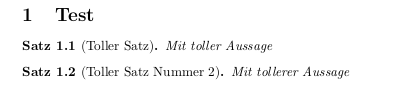
\includegraphics[width=0.8\textwidth]{images/satz.png}}}

\end{frame}
%\section{Referenzen}

\subsection{ und Literaturverzeichnis}


\begin{frame}[fragile,t]
\frametitle{Bibliographien mit \texttt{thebibliography}}
\begin{itemize}[<+->]
  \item \textbf{Eine} einfache Möglichkeit in LaTeX eine Bibliographie zu erstellen.
  \item Dieses Vorgehen hat den Vorteil, dass im Gegensatz zu BibTeX \textbf{\texttt{<Inhalt der Referenz>}} den eingenen Ansprüchen entsprechend, einfach formatiert werden kann.
  \begin{enumerate}[<+->]
\item Einfügen der \texttt{thebibliography}-Umgebung vor \texttt{$\backslash$end\{document\}}
  \begin{center}
  \lstinline[style=Latex]+\begin{thebibliography}{99}+\\
  $\vdots$\\
   \lstinline[style=Latex]+\end{thebibliography}+
  \end{center}
  \item Erstellen von Einträgen innerhalb dieser Umgebung durch:
  \begin{center}
  \lstinline[style=Latex]+\bibitem{<Referenzname>} <Inhalt der Referenz>+
  \end{center}
  \item Aufrufen der Literaturangaben im Text durch
  \begin{center}
  \lstinline[style=Latex]+\cite{<Referenzname>}+ 
  \end{center}
  \end{enumerate}
\end{itemize} 
\end{frame}

\begin{frame}[fragile,t]
\frametitle{Beispiel mit einer Referenz}
\begin{lstlisting}[style=Latex]
\documentclass[12pt]{article}
\begin{document}
This thesis bases on the empirical work of Frumkes \cite{brain}.

\begin{thebibliography}{99}
\bibitem{brain} Lewis B. Frumkes. (2001). ``\textit{How to Raise Your I.Q. by Eating Gifted Children}.'' iUniverse.
\end{thebibliography}
\end{document}
\end{lstlisting}
\end{frame}

\begin{frame}[fragile]
\frametitle{Beispiel Literaturangabe}
\result{
\begin{figure}[htbp]
    \centering
        %trim=left botm right top
        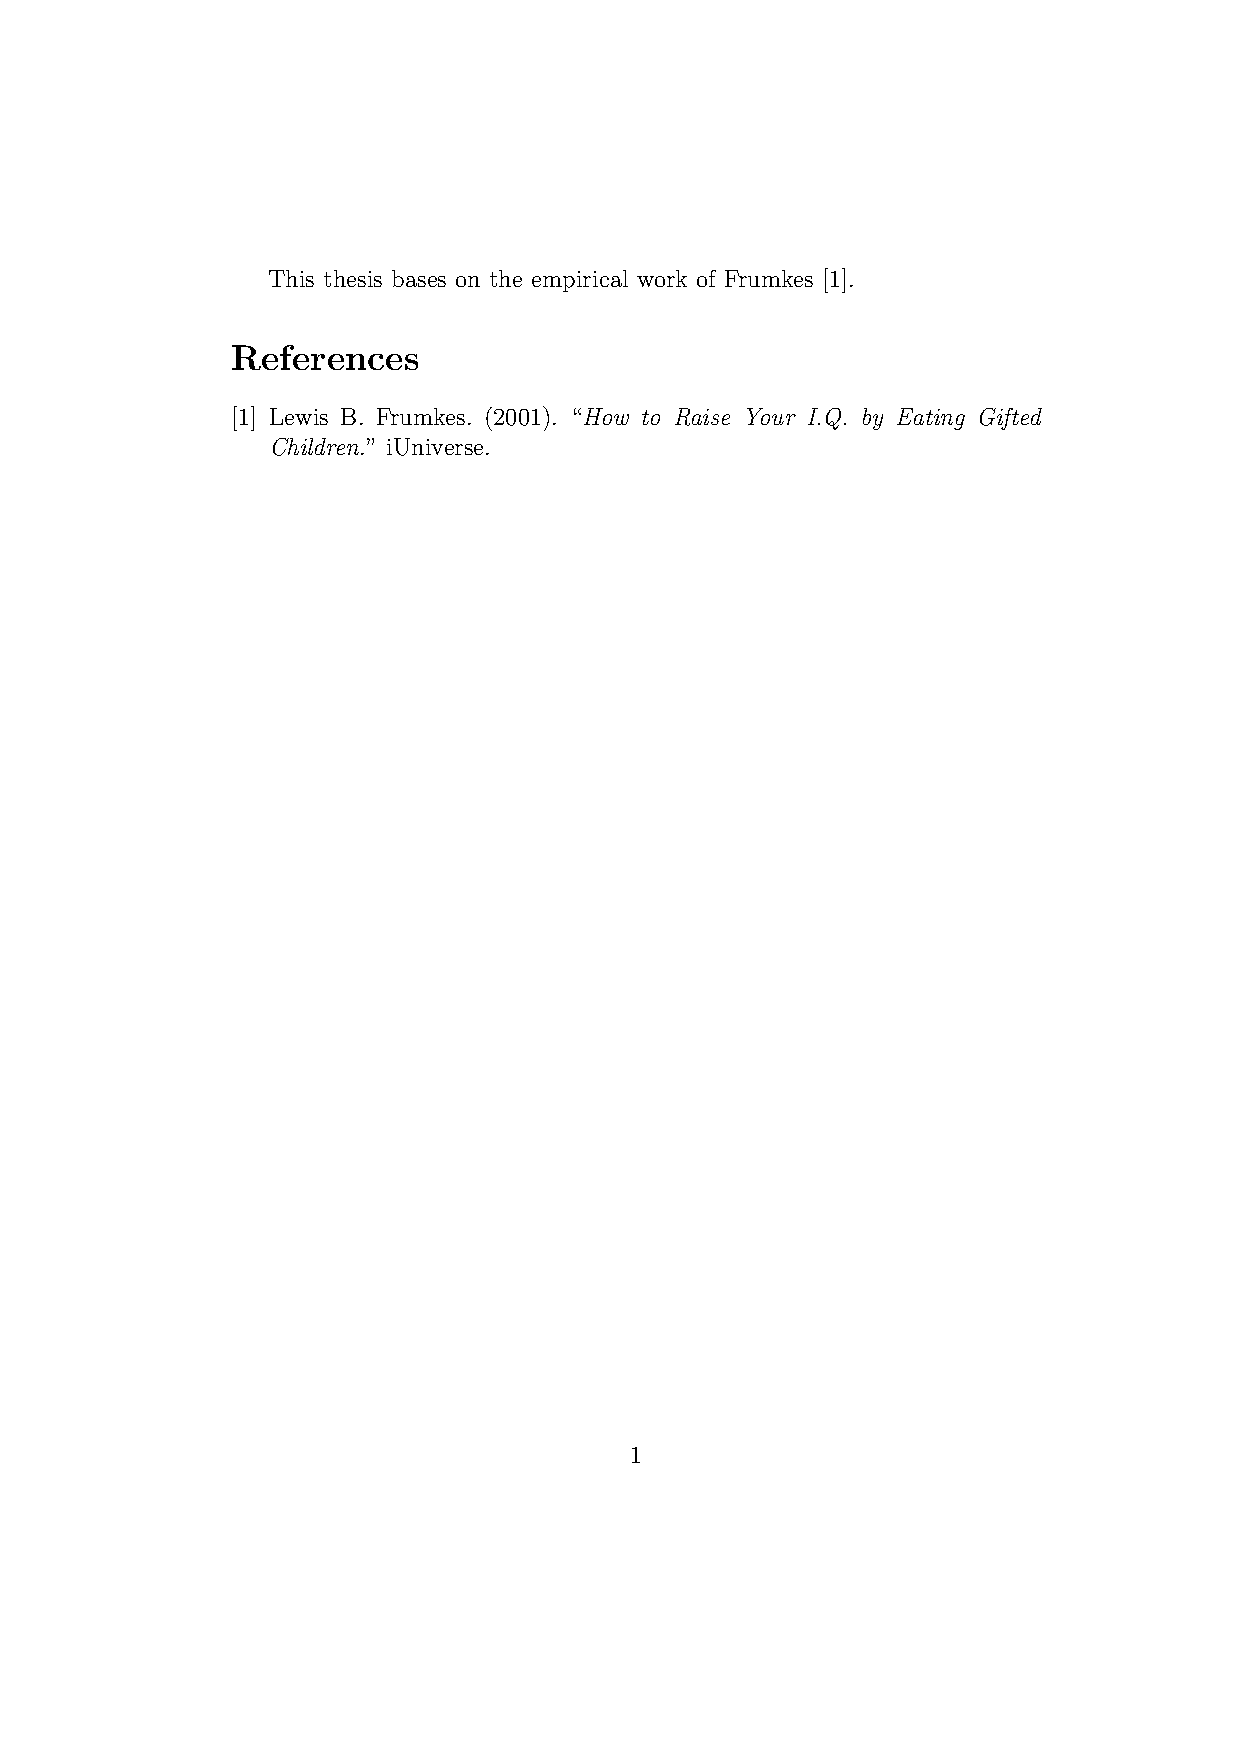
\includegraphics[clip, trim=3cm 22cm 0.5cm 4cm, width=1.00\textwidth]{images/Literaturangabe1.pdf}
    %\caption{Title}
    %\label{fig:somthing}
\end{figure}}
\end{frame}


\begin{frame}[fragile,t]
\frametitle{Beispiel mit mehreren Referenzen}
\begin{lstlisting}[style=Latex]
\documentclass[12pt]{article}
\begin{document}
This thesis bases on the empirical work of Frumkes \cite{brain}. The next theorem shows how to earn more money if you sell bulk trash. This work is founded by Dennis and Matthias \cite{money}.

\begin{thebibliography}{99}
\bibitem{brain} Lewis B. Frumkes. (2001). ``\textit{How to Raise Your I.Q. by Eating Gifted Children}.'' iUniverse.
\bibitem{money} Dennis K., Matthias D. (2017). ``\textit{How we earn more money}.'' Fachschaft VWL.
\end{thebibliography}
\end{document}
\end{lstlisting}
\end{frame}

\begin{frame}[fragile]
\frametitle{Beispiel Literaturangabe}
\result{
\begin{figure}[htbp]
    \centering
        %trim=left botm right top
        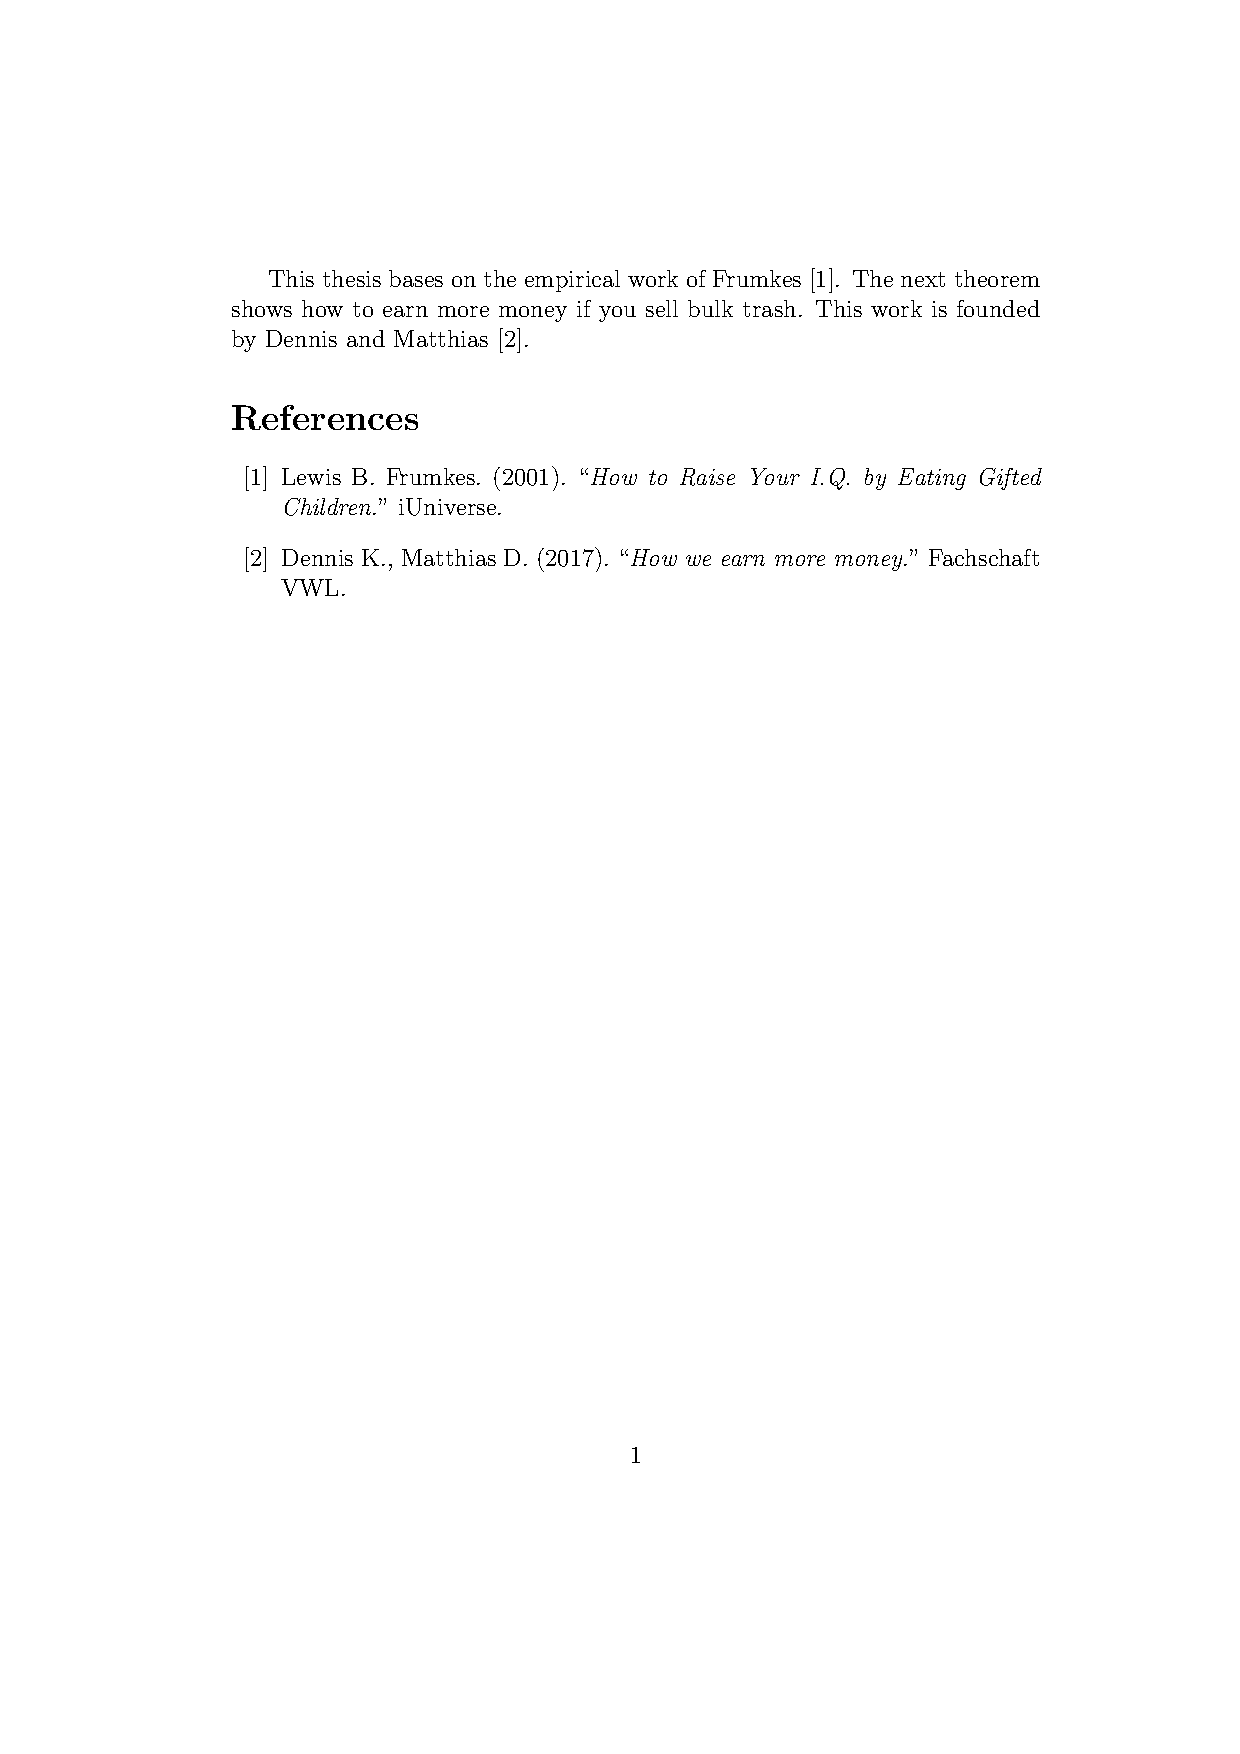
\includegraphics[clip, trim=3cm 19.5cm 0.5cm 4cm, width=1.00\textwidth]{images/Literaturangabe2.pdf}
    %\caption{Title}
    %\label{fig:somthing}
\end{figure}}
\end{frame}

\begin{frame}[fragile,t]
\frametitle{Andere Referenzstile}
Referenzieren mit Autor und Jahr in einer Klammer im Text \texttt{(<Autor>, Jahr)}:
\begin{itemize}[<+->] 
  \item In der Präambel müssen die folgenden Einträge vorgenommen werden:
   \begin{center}\lstinline[style=Latex]+\usepackage[authoryear]{natbib}+\end{center}
   \begin{center}\lstinline[style=Latex]+\setcitestyle{notesep={: }}+\end{center}
  \item In der Bibliographie muss jetzt der Inhalt der verweisenden Referenz angegeben werden: 
   \begin{center}\lstinline[style=Latex]+\bibitem[Autor/Autoren(Jahr)]{<Referenzname>} <Inhalt der Referenz>+\end{center}
   \item jetzt kann der Eintrag im eigentlichen Text referenziert werden: (\lstinline[style=Latex]+\citep+ muss verwendet werden)
    \begin{center}\lstinline[style=Latex]+\citep{<Referenzname>}+\end{center}
\end{itemize}
\end{frame}


\begin{frame}[fragile,t]
\frametitle{Beispiel andere Referenzstile}\vspace{-10pt}
\begin{lstlisting}[style=Latex]
\documentclass[12pt]{article}
\usepackage[authoryear]{natbib}
\setcitestyle{notesep={: }}

\begin{document}
This thesis bases on the empirical work of Frumkes \citep{brain}. The next theorem shows how to earn more money if you sell bulk trash. This work is founded by Dennis and Matthias \citep{money}.
\begin{thebibliography}{99}
\bibitem[Frumkes(2001)]{brain} Lewis B. Frumkes. (2001). ``\textit{How to Raise Your I.Q. by Eating Gifted Children}.'' iUniverse.
\bibitem[Dennis and Matthias(2017)]{money} Dennis K., Matthias D. (2017). ``\textit{How we earn more money}.'' Fachschaft VWL.
\end{thebibliography}
\end{document}
\end{lstlisting}
\end{frame}

\begin{frame}[fragile,t]
\frametitle{Beispiel andere Referenzstile}
\result{
\begin{figure}[htbp]
    \centering
        %trim=left botm right top
        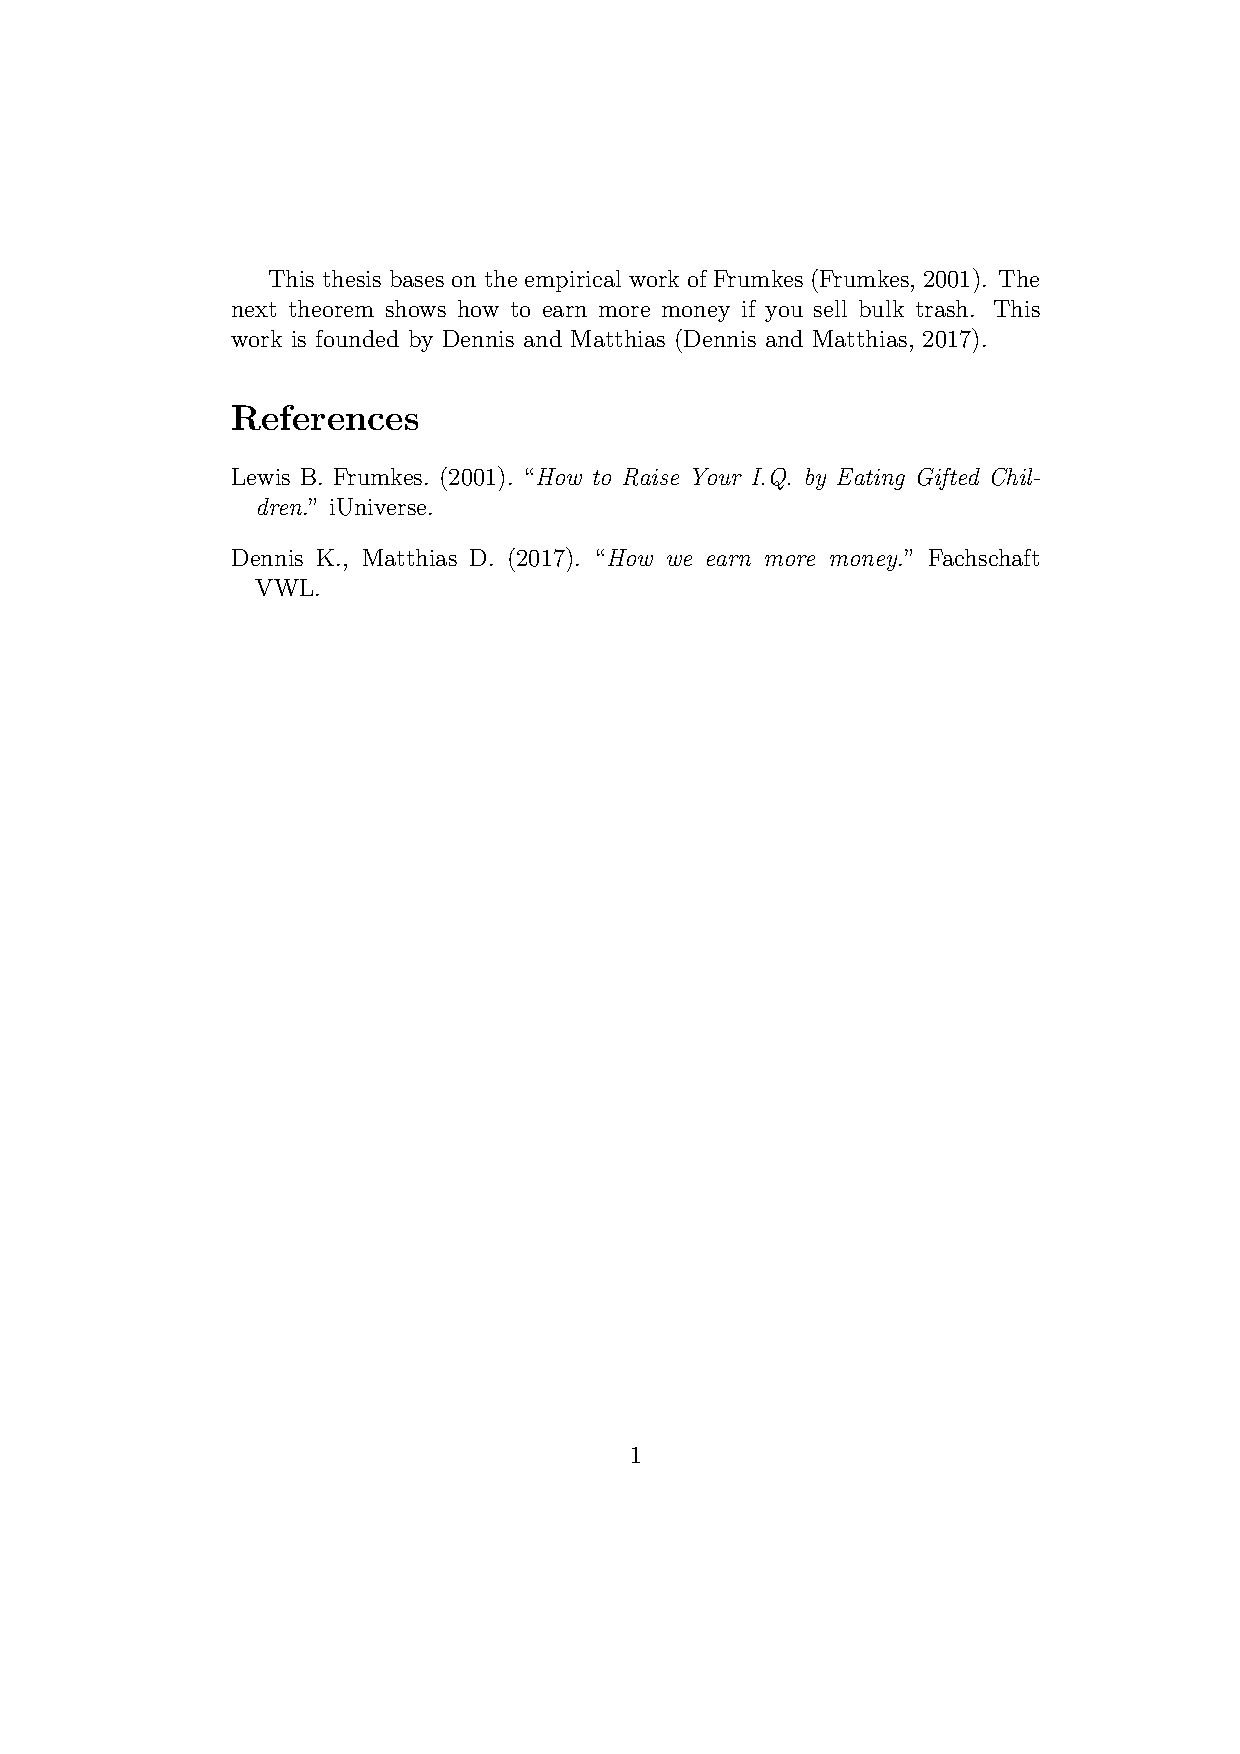
\includegraphics[clip, trim=3cm 19.5cm 0.5cm 4cm, width=1.00\textwidth]{images/Literaturangabe3.pdf}
    %\caption{Title}
    %\label{fig:somthing}
\end{figure}}
\end{frame}

\begin{frame}[fragile,t]
\frametitle{Zu beachten bei der Verwendung von \texttt{thebibliography}}
\begin{itemize}
\item Die Reihenfolge der \lstinline[style=Latex]+\bibitem+ Einträge legt die die Reihenfolge im LaTeX~Dokument fest
\item Die Bibliographieeinträge müssen alle von Hand formatiert werden
\item Bei Umfangreicheren Bibliographien sollte Biblatex verwendet werden. Dies führt jedoch auch zu mehr Aufwand. Wir verweisen hier auf entsprechende Seiten im Internet.
\end{itemize}
\end{frame}



\subsection{Referenzieren von Objekten}

\begin{frame}[fragile]
\frametitle{Referenzen}
\begin{itemize}[<+->]
  \item \LaTeX kann ''Verlinkungen'' zu table und figure-Umgebungen und Gleichungen erstellen
  \item Damit kann im Text auf die Nummerierung der Elemente zugegriffen werden
    \begin{itemize}[<+->]
      \item \lstinline[style=Latex]+\label{<Bezeichnung>}+ Dazu müssen die zu referenzierende Elemente mittels  ''verankert'' werden
      \item \lstinline[style=Latex]+\ref{<Bezeichnung>}+ Jetzt können diese durch abgefragt werden. 
      \item \lstinline[style=Latex]+\eqref{<Bezeichnung>}+ Handelt es sich um eine Gleichung, so kann  verwendet werden
    \end{itemize}
  \end{itemize}
\end{frame}


\begin{frame}[fragile]
\frametitle{Beispiel- ERSETZEM DURCH FIGURE ung gleichung}
\begin{lstlisting}[style=Latex]
\begin{satz}[genialer Satz]\label{satz:genial}
Dieser beinhaltet eine Formel:
\begin{equation}\label{eq:toll}
a^2 + b^2 = c^2
\end{equation}
\end{satz}
Satz \ref{satz:genial}, namentlich "`\nameref{satz:genial}"' 
auf Seite \pageref{satz:genial} beinhaltet die Formel \eqref{eq:toll}.
\end{lstlisting}
\pause
\end{frame}

\begin{frame}[fragile]
\frametitle{Beispiel}
\begin{satz}[genialer Satz]\label{satz:genial}
Dieser beinhaltet eine Formel:
\begin{equation}\label{eq:toll}
a^2 + b^2 = c^2
\end{equation}
\end{satz}
Satz \ref{satz:genial}, namentlich "`\nameref{satz:genial}"' 
auf Seite \pageref{satz:genial} beinhaltet die Formel \eqref{eq:toll}.
\end{frame}


\subsection{Fußnoten}

\begin{frame}[fragile]
\frametitle{Fußnoten}
\begin{itemize}[<+->]
  \item Fußnoten werden mittels \lstinline[style=Latex]+\footnote[<Nummer>]{<Text>}+ erzeugt.
  \item durch einen neuen \lstinline[style=Latex]+\chapter+ wird der Fußnotenzähler resettet.
  \item Es können auch andere Fußnotensymbole verwendet werden:
   \lstinline[style=Latex]+\renewcommand{\thefootnote}{\<ZiffStil>{footnote}}+ \\
   Dabei sind alle Ziffernstile, die auch für die Seitennummerierung gelten, sowie \texttt{fnysmbol} gültig.
\end{itemize}\pause
Beispiel:
\begin{lstlisting}[style=Latex]
Das ist ein toller Text\footnote{das die Notiz dazu}
\renewcommand{\thefootnote}{\fnysmbol{footnote}}
Das ist ein noch besserer Text\footnote{so sehen Symbole aus}
\renewcommand{\thefootnote}{\alph{footnote}}
Dies ist der letzte Text\footnote{mit Buchstaben}
\end{lstlisting}
Das ist ein toller Text\footnote{das die Notiz dazu}
\renewcommand{\thefootnote}{\fnsymbol{footnote}}
Das ist ein noch besserer Text\footnote{so sehen Symbole aus}
\renewcommand{\thefootnote}{\alph{footnote}}
Dies ist der letzte Text\footnote{mit Buchstaben}
\end{frame}

\begin{frame}[fragile]
\frametitle{Fußnoten}
\begin{itemize}[<+->]
  \item in manchen Fällen ist es Sinnvoll, Fußnote und Fußnotentext getrennt voneinander zu erstellen
  \item eine Fußnote kann manuell mit \lstinline[style=Latex]+\footnotemark[<Nummer>]+ erstellt werden
  \item wird keine Nummer angegeben, so wird der aktuelle Zähler um eins erhöht und als Fußnote verwendet. Die Angabe eine Nummer lässt den Zähler unberührt.
  \item über \lstinline[style=Latex]+\footnotetext[<Nummer>]{<Text>}+ kann ein Text erstellt werden. \texttt{<Nummer>} verhält sich hier genau wie oben.
  \item über diesen Weg lassen sich Fußnoten nahezu überall erstellen
\end{itemize}
\end{frame}

\begin{frame}[fragile]
\frametitle{Beispiel}
\begin{lstlisting}[style=latex]
Wir setzten eine Footnote \footnotemark[12] ...  
aber zeigen Sie auf einer anderen seite an.
\end{lstlisting}
Wir setzten eine Footnote \footnotemark[12] ...  
aber zeigen Sie auf einer anderen seite an
\end{frame}
\begin{frame}[fragile]
\begin{lstlisting}[style=latex]
\footnotetext[12]{hier}
\end{lstlisting}
\end{frame}
\footnotetext[12]{hier}

\subsection{Inhaltsverzeichnis}

\begin{frame}[fragile]
\frametitle{Inhaltsverzeichnis}
\begin{itemize}[<+->]
  \item mit dem Befehl \lstinline[style=Latex]+\tableofcontents+ wird eine \texttt{.toc}-Datei erstellt, in der alle Abschnitte aufgelistet werden
  \item beim erneuten compilieren wird diese Datei eingelesen und als Inhaltsverzeichnis ausgegeben
  \item<+-|alert@3> daher immer 2x compilieren! (3x bei langen Inhaltsverzeichnis)
  \item über den Befehl \lstinline[style=Latex]+\addtocontents{toc}{Eintrag}+ lässt sich manuell ein Eintrag in der \texttt{.toc}-Datei einfügen.\\
  \item über \lstinline[style=Latex]+\listoffigures+ oder \lstinline[style=Latex]+\listoftables+ lassen sich entsprechend analog Figuren- bzw. Tabellenverzeichnisse erstellen
  \item die Tiefe des Inhaltsverzeichnis wird über die Variable \texttt{tocdepth} gesteuert
\end{itemize}
\begin{lstlisting}[style=Latex]
\setcounter{tocdepth}{2}
\end{lstlisting}
\end{frame}

\subsection{Hyperref}

\begin{frame}[fragile]
\frametitle{Hyperref}
\begin{itemize}[<+->]
  \item das Paket \texttt{hyperref} sorgt dafür, dass Verlinkungen in \LaTeX\, anklickbare Hyperlinks erzeugen.
  \item dadurch werden die Befehle \lstinline[style=Latex]+\url{<URL>}+ bzw. \lstinline[style=Latex]+\href{<URL>}{<Text>}+ bereitgestellt, mit dem Internetadressen angegeben werden können
  \item außerdem wird der Befehl \lstinline[style=Latex]+\hypersetup+ definiert, mit dem Linkfarbe, PDF-Author und viele andere Dinge einstellbar sind. Weiteres dazu unter \url{http://en.wikibooks.org/wiki/LaTeX/Hyperlinks}
\end{itemize}
\end{frame}

\begin{frame}[fragile]
\textbf{Achtung:} Verwendet Ihr Hyperrefs in einem article Dokument, werden alle Links rot umrandet. Dies könnt unterbinden indem ihr Hyperref so einbindet:

\begin{lstlisting}[style=Latex]
\usepackage[colorlinks=false,pdfborder={0 0 0}]{hyperref}%Hide RED PDF Border
\end{lstlisting}

\end{frame}


%\section{Weiteres}

\subsection{selber definieren}

\begin{frame}[fragile]
\frametitle{Befehle definieren}
\begin{itemize}[<+->]
  \item mit \lstinline[style=Latex]+\newcommand{\<Befehl>}[<AnzArgs>][<Std>]{<wastun>}+ können eigene Befehle definiert werden
  \item Befehlsnamen dürfen nur aus Buchstaben bestehen
  \item mit \texttt{<AnzArgs>} kann die Anzahl der übergebenen Argumente festgelegt werden. Diese können dann mit \lstinline[style=Latex]+#1+, \lstinline[style=Latex]+#2+, \ldots abgerufen werden.
  \item mit \texttt{<Std>} kann ein Standardwert für das erste Argument gegeben werden. Dadurch wird dieses optional.
  \item \lstinline[style=Latex]+\renewcommand+ überschreibt einen bestehenden Befehl
  \item durch \lstinline[style=Latex]+\ensuremath+ wird der Befehl falls nötig in den Mathematikmodus versetzt
\end{itemize}
\end{frame}

\begin{frame}[fragile]
\frametitle{Beispiel -- Befehle}
\begin{lstlisting}[style=Latex]
\newcommand\eps{\ensuremath\varepsilon}
\newcommand\cboxes[2]{
  \begin{center}
    \begin{tabular}{|c|c|}\hline #1 & #2 \\\hline\end{tabular}
  \end{center}
}
\eps \\
\cboxes{Hallo}{Welt}
\end{lstlisting}
\newcommand\eps{\ensuremath\varepsilon}
\newcommand\cboxes[2]{
  \begin{center}
    \begin{tabular}{|c|c|}\hline #1 & #2 \\\hline\end{tabular}
  \end{center}
}
\eps \\
\cboxes{Hallo}{Welt}
\end{frame}



\subsection{Folien}

\begin{frame}[fragile]
\frametitle{Folien}
\begin{itemize}[<+->]
  \item als Dokumentklasse muss \texttt{beamer} verwendet werden
  \item es stehen viele verschiedene Themes zur Auswahl, einen Überblick erhält man unter \url{http://www.namsu.de/latex/themes/uebersicht_beamer.html} \\
    Diese werden mit \lstinline[style=Latex]+\usetheme{<Themenname>}+ aktiviert
  \item verwendet man \texttt{beamer} mit der Option \texttt{handout} werden alle Übergänge deaktiviert

\end{itemize}
\end{frame}

\begin{frame}[fragile]
\frametitle{frame-Umgebung}
\begin{itemize}[<+->]
  \item jede Folie ist in der Beamer-Klasse eine \texttt{frame}-Umgebung oder alternativ durch \lstinline[style=Latex]+\frame{<Inhalt>}+.
  \item mit \lstinline[style=Latex]+\frametitle{<Titel>}+ kann der Seitentitel festgelegt werden
  \item einen Untertitel erhält man mit \lstinline[style=Latex]+\subtitle{<Untertitel>}+
  \item eine vorgefertigte Titelseite erhält man mittels \lstinline[style=Latex]+\titlepage+
\end{itemize}
\end{frame}

\begin{frame}[fragile]
\frametitle{Overlays}
\begin{itemize}[<+->]
  \item der Befehl \lstinline[style=Latex]+\pause+ erzeugt eine Folie mit dem Inhalt bis zur Pause und eine weitere mit der gesamten Seite
  \item Aufzählungen erhalten als zusätzlichen optionalen Parameter \lstinline[style=Latex]+<<Pausenart>>+.\\
    Dabei bedeutet eine Zahl $n$, dass etwas in Folie $n$ passiert, ein ``+'' deckt das Item auf oder verdeckt es und ein ``-'' lässt es bestehen, ``alert@$n$'' markiert das Item in Folie $n$. Mit ``|'' können mehrere Anweisungen hintereinander stehen.
  \item steht eine Pausenart als optionaler Parameter an der Aufzählungsumgebung, so gilt dies für die gesamte Aufzählung inkl. Unteraufzählungen.
\end{itemize}
\end{frame}

\begin{frame}[fragile]
\frametitle{Beispiel}\vspace{-5pt}
\begin{lstlisting}[style=Latex]
\begin{itemize}
  \item Einleitung
  \item<2-> daher
  \item<3-|alert@3> aber Achtung!
  \item<4> ist nur in 4 da
  \item<5-> Schlussfolgerung
\end{itemize}
\end{lstlisting}\vspace{-25pt}\pause
\begin{itemize}
  \item Einleitung
  \item<2-> daher
  \item<3-|alert@3> aber Achtung!
  \item<4> ist nur in 4 da
  \item<5-> Schlussfolgerung
\end{itemize}
\end{frame}


\begin{frame}\frametitle{mehr zur Klasse Beamer}
\url{http://www.ctan.org/tex-archive/macros/latex/contrib/beamer/doc/beameruserguide.pdf}
\end{frame}

\end{document}